%%
% Είδος: διπλωματική στα αγγλικά
\documentclass{uthece-thesis} 

% Πακέτα και ορισμοί που τυχόν χρειάζονται, ανάλογα με το κείμενο της διπλωματικής
\usepackage{algorithm}      % float wrapper: caption, numbering, [H]
\usepackage{algpseudocode}  % the algorithmicx syntax (mixed case)
\usepackage[hyphens]{url}
\usepackage{multicol}
\usepackage{multirow}
\usepackage[table]{xcolor}
\usepackage{caption} 
\captionsetup[table]{skip=10pt}
\usepackage{tikz}
\usepackage{datetime}
\usepackage{ifthen}
\usepackage{hyperref} % Για ενεργά URLs
\usepackage{graphicx}
\usepackage{caption}
\usepackage{subcaption} % Add this line
\usepackage{enumitem}
\usepackage{listings}
\usepackage{pgfplots}
\pgfplotsset{compat=1.18}

\usepackage{caption}
\captionsetup[figure]{labelfont=it,textfont=it}
\captionsetup[table]{labelfont=it,textfont=it}

\usepackage[strict]{changepage}

\usepgfplotslibrary{external}

% Πρόσθετοι ορισμοί, ανάλογα με το κείμενο της διπλωματικής
% typeset source code
\newcommand{\src}[1]{{\tt#1}}

% typeset a backslash
\newcommand{\bkslash}{\symbol{92}}

% Κύρια γλώσσα της διπλωματικής
% μην την τροποποιείτε
\ifgrthesisoption 
    \setlanguage{greek}
\else
    \setlanguage{american} 
\fi

%%%%%%%%%%%%%%%%%%%%%%%%%%%%%%%%%%%%%%%%%%%%%%%%%%%%%
%% THESIS INFO / ΠΛΗΡΟΦΟΡΙΕΣ ΔΙΠΛΩΜΑΤΙΚΗΣ
%%
% Τίτλος Διπλωματικής Εργασίας στα ελληνικά
	\title{ΤΙΤΛΟΣ ΔΙΠΛΩΜΑΤΙΚΗΣ ΜΕ ΜΙΚΡΑ H ΚΕΦΑΛΑΙΑ ΓΡΑΜΜΑΤΑ, ΣΤΟΙΧΙΣΜΕΝΟΣ ΣΤΟ ΚΕΝΤΡΟ}
% Τίτλος Διπλωματικής Εργασίας στα αγγλικά
	\titleEng{ΤITLE OF THESIS IN SMALL OR CAPITAL LETTERS, CENTERED}
% Ονοματεπώνυμο φοιτητή στα ελληνικά
	\edef\authorname{Ον/μο Φοιτητή}
	\edef\secauthorname{Ον/μο 2ου Φοιτητή} % κενό αν η εργασία έγινε από έναν φοιτητή
% Ονοματεπώνυμο φοιτητή στα αγγλικά 
	\edef\authornameEng{Name Surname of student}
	\edef\secauthornameEng{Name Surname of 2nd student} % κενό αν η εργασία έγινε από έναν φοιτητή
% Ονοματεπώνυμο Επιβλέποντα Καθηγητή στα ελληνικά
	\supervisor{Ονοματεπώνυμο Επιβλέποντα}
% Ονοματεπώνυμο Επιβλέποντα Καθηγητή στα αγγλικά
	\supervisorEng{Name Surname of Supervisor}
% Φύλλο επιβλέποντα στα ελληνικά 
% Μην το τροποποιείτε για διπλωματική στα αγγλικά
	\edef\supervisorMaleFemale{Επιβλέπων/πουσα}
% Στοιχεία επιτροπής στα αγγλικά
    \edef\supervisortitle{Rank/position of Supervisor}
    \edef\supervisoraffiliation{Department of Electrical and Computer Engineering, University of Thessaly}
    \edef\memberonename{Name Surname of Member 1}
    \edef\memberonetitle{Rank/position of Member 1}
    \edef\memberoneaffiation{Department/Institution of Member 1}
    \edef\membertwoname{Name Surname of Member 2}
    \edef\membertwotitle{Rank/position of Member 2}
    \edef\membertwoaffiation{Department/Institution of Member 2}    
% Ημερομηνία υποβολής διπλωματικής
    \newdate{docdate}{04}{02}{2022}
% Ημερομηνία έγκρισης διπλωματικής
    \newdate{docapprovedate}{24}{02}{2022}
% format ημερομηνίας - μην το τροποποιείτε
    \newdateformat{mydate}{\THEDAY-\THEMONTH-\THEYEAR} \mydate
% Τόπος και έτος διπλωματικής στα ελληνικά
	\edef\thesisPlaceDate{Μήνας \getdateyear{docdate}}
% Τόπος και έτος διπλωματικής στα αγγλικά
	\edef\thesisPlaceDateEng{Month \getdateyear{docdate}}
%
%%%%%%%%%%%%%%%%%%%%%%%%%%%%%%%%%%%%%%%%%%%%%%%%%%%%

\raggedbottom
\begin{document}

\frontmatter
\maketitle


%%%%%%%%%%%%%%%%%%%%%%%%%%%%%%%%%%%%%%%%%%%%%%%%%%%%%
%% OPTIONAL MATERIAL / ΠΡΟΑΙΡΕΤΙΚΕΣ ΕΝΟΤΗΤΕΣ
%%
% Κατάλογος Σχημάτων προαιρετικά
	\listoffigures % σε σχόλια για μη εμφάνιση
% Κατάλογος Πινάκων προαιρετικά
	\listoftables % σε σχόλια για μη εμφάνιση
% Συντομογραφίες - Αρκτικόλεξα - Ακρωνύμια προαιρετικά
	% Συντομογραφίες - Αρκτικόλεξα - Ακρωνύμια

\newcommand{\abbrev}[2]{#1 \> #2\\ }
\begin{abbreviations}

\begin{tabbing}
%ta 'a' rythmizoun to platos ton dyo stilon
  aaaaaaaaaaaaaaaaa \= aaaaaaaaaaaaaaaaaaaaaa\kill
  \abbrev{BRAM}{Block Random Access Memory}
  \abbrev{CSA}{Carry-Save Adder}
  \abbrev{CSAM}{Carry-Save Array Multiplier}
  \abbrev{CSHM}{Computation-Sharing Hardware Multiplier}
  \abbrev{dB}{Decibel}
  \abbrev{DFT}{Discrete Fourier Transform}
  \abbrev{DSP}{Digital Signal Processing}
  \abbrev{FFT}{Fast Fourier Transform}
  \abbrev{FPGA}{Field-Programmable Gate Array}
  \abbrev{FT}{Fourier Transform}
  \abbrev{LUT}{Look-Up Table}
  \abbrev{LUTRAM}{Look-Up Table Random Access Memory}
  \abbrev{MAC}{Multiply-Accumulate}
  \abbrev{MDF}{Multi-Path Delay Feedback}
  \abbrev{SDF}{Single-Path Delay Feedback}
  \abbrev{SQNR}{Signal-to-Quantization-Noise Ratio}
  \abbrev{SRFFT}{Split-Radix Fast Fourier Transform}
  \abbrev{DIT}{Decimation-In-Time}
\end{tabbing}
\end{abbreviations} % σε σχόλια για μη εμφάνιση 
%
%%%%%%%%%%%%%%%%%%%%%%%%%%%%%%%%%%%%%%%%%%%%%%%%%%%%


\mainmatter
%%%%%%%%%%%%%%%%%%%%%%%%%%%%%%%%%%%%%%%%%%%%%%%%%%%%%
%% CHAPTERS / ΚΕΦΑΛΑΙΑ 
%%
    \chapter{Εισαγωγή}
\label{chap1}

Εδώ αυτή κάνουμε μια γενική περιγραφή του χώρου εφαρμογής της διπλωματικής. Αναφέρουμε τα χαρακτηριστικά του χώρου και καταλήγουμε στα γενικότερα προβλήματα που αντιμετωπίζει ο χώρος. Η συζήτηση των προβλημάτων θα πρέπει να προϊδεάζει τον αναγνώστη για το τι θα προσπαθήσει να αντιμετωπίσει η διπλωματική, χωρίς ακόμα να αναφερόμαστε συγκεκριμένα στο αντικείμενο της διπλωματικής.
  


\section{Αντικείμενο της διπλωματικής}

Εδώ αναφερόμαστε συγκεκριμένα στο τί θα κάνει η διπλωματική. Αναφέρουμε λεπτομερώς α) τα προβλήματα που θα λύσει (και που ήδη έχουν περιγραφεί γενικά στην προηγούμενη ενότητα), και β) πώς σκοπεύει να τα λύσει. 
Είναι σημαντικό κάποιος που θα διαβάσει την ενότητα αυτή να καταλάβει σε σημαντικό βαθμό τον σκοπό της διπλωματικής σας και τις τεχνικές δυσκολίες της, χωρίς να είναι αναγκαίο να δει όλα τα άλλα κεφάλαια. Η ενότητα αυτή θέλει πολύ προσοχή και καλύτερα να τη γράψετε αφού έχετε γράψει όλα τα υπόλοιπα κεφάλαια.

\subsection{Συνεισφορά}
Εδώ παραθέτουμε αριθμητικά συγκεκριμένες ενέργειες/λύσεις/μεθοδολογίες που παρουσιάζει η διπλωματική και λύνουν τα προβλήματα που υποσχεθήκαμε στην προηγούμενη ενότητα ότι θα λύσει η διπλωματική. Συνήθως η υποενότητα αυτή έχει την παρακάτω μορφή:

Η συνεισφορά της διπλωματικής συνοψίζεται ως εξής:
\begin{enumerate}
\item Μελετήθηκαν συστήματα κ.λ.π.
\item Υλοποιήθηκαν τρεις αλγόριθμοι υπολογισμού κ.λ.π.
\item Αξιολογήθηκε η επίδοση των αλγορίθμων και βρέθηκε ότι κ.λ.π.
\item Ενσωματώθηκαν οι αλγόριθμοι σε πρότυπο σύστημα κ.λ.π.
\item ...
\end{enumerate}


\section{Οργάνωση του τόμου}

Εδώ περιγράφουμε τα κεφάλαια της διπλωματικής: μία πρόταση για το τί θα έχει  κάθε κεφάλαιο.Συνήθως η ενότητα αυτή έχει την παρακάτω μορφή (δεν θα σας πάρει πάνω από μία μεγάλη παράγραφο):

Εργασίες σχετικές με το αντικείμενο της διπλωματικής παρουσιάζονται στο Κεφάλαιο \ref{chap2}. Το Κεφάλαιο ... συζητά θέματα μοντελοποίησης. Στο Κεφάλαιο ... αναπτύσσουμε κ.λ.π. 

Για την τελική οργάνωση του κειμένου σας, συμβουλευθείτε τον επιβλέποντα της εργασίας.



    \chapter{Background and Theoretical Foundations}
\label{Background}

\section{Introduction to Fourier Transform}
In mathematics, the Fourier transform (FT) is an integral transform that acts on a function to reveal its frequency components. It takes an input function and generates a new, complex-valued function that details the intensity of different frequencies present in the original. The term ``Fourier transform'' applies to both the mathematical process itself and the resulting function. To distinguish between the two, the output is often referred to as the ``frequency domain'' representation~\cite{oppenheim2010}.. 

\begin{figure}[H]
    \centering
    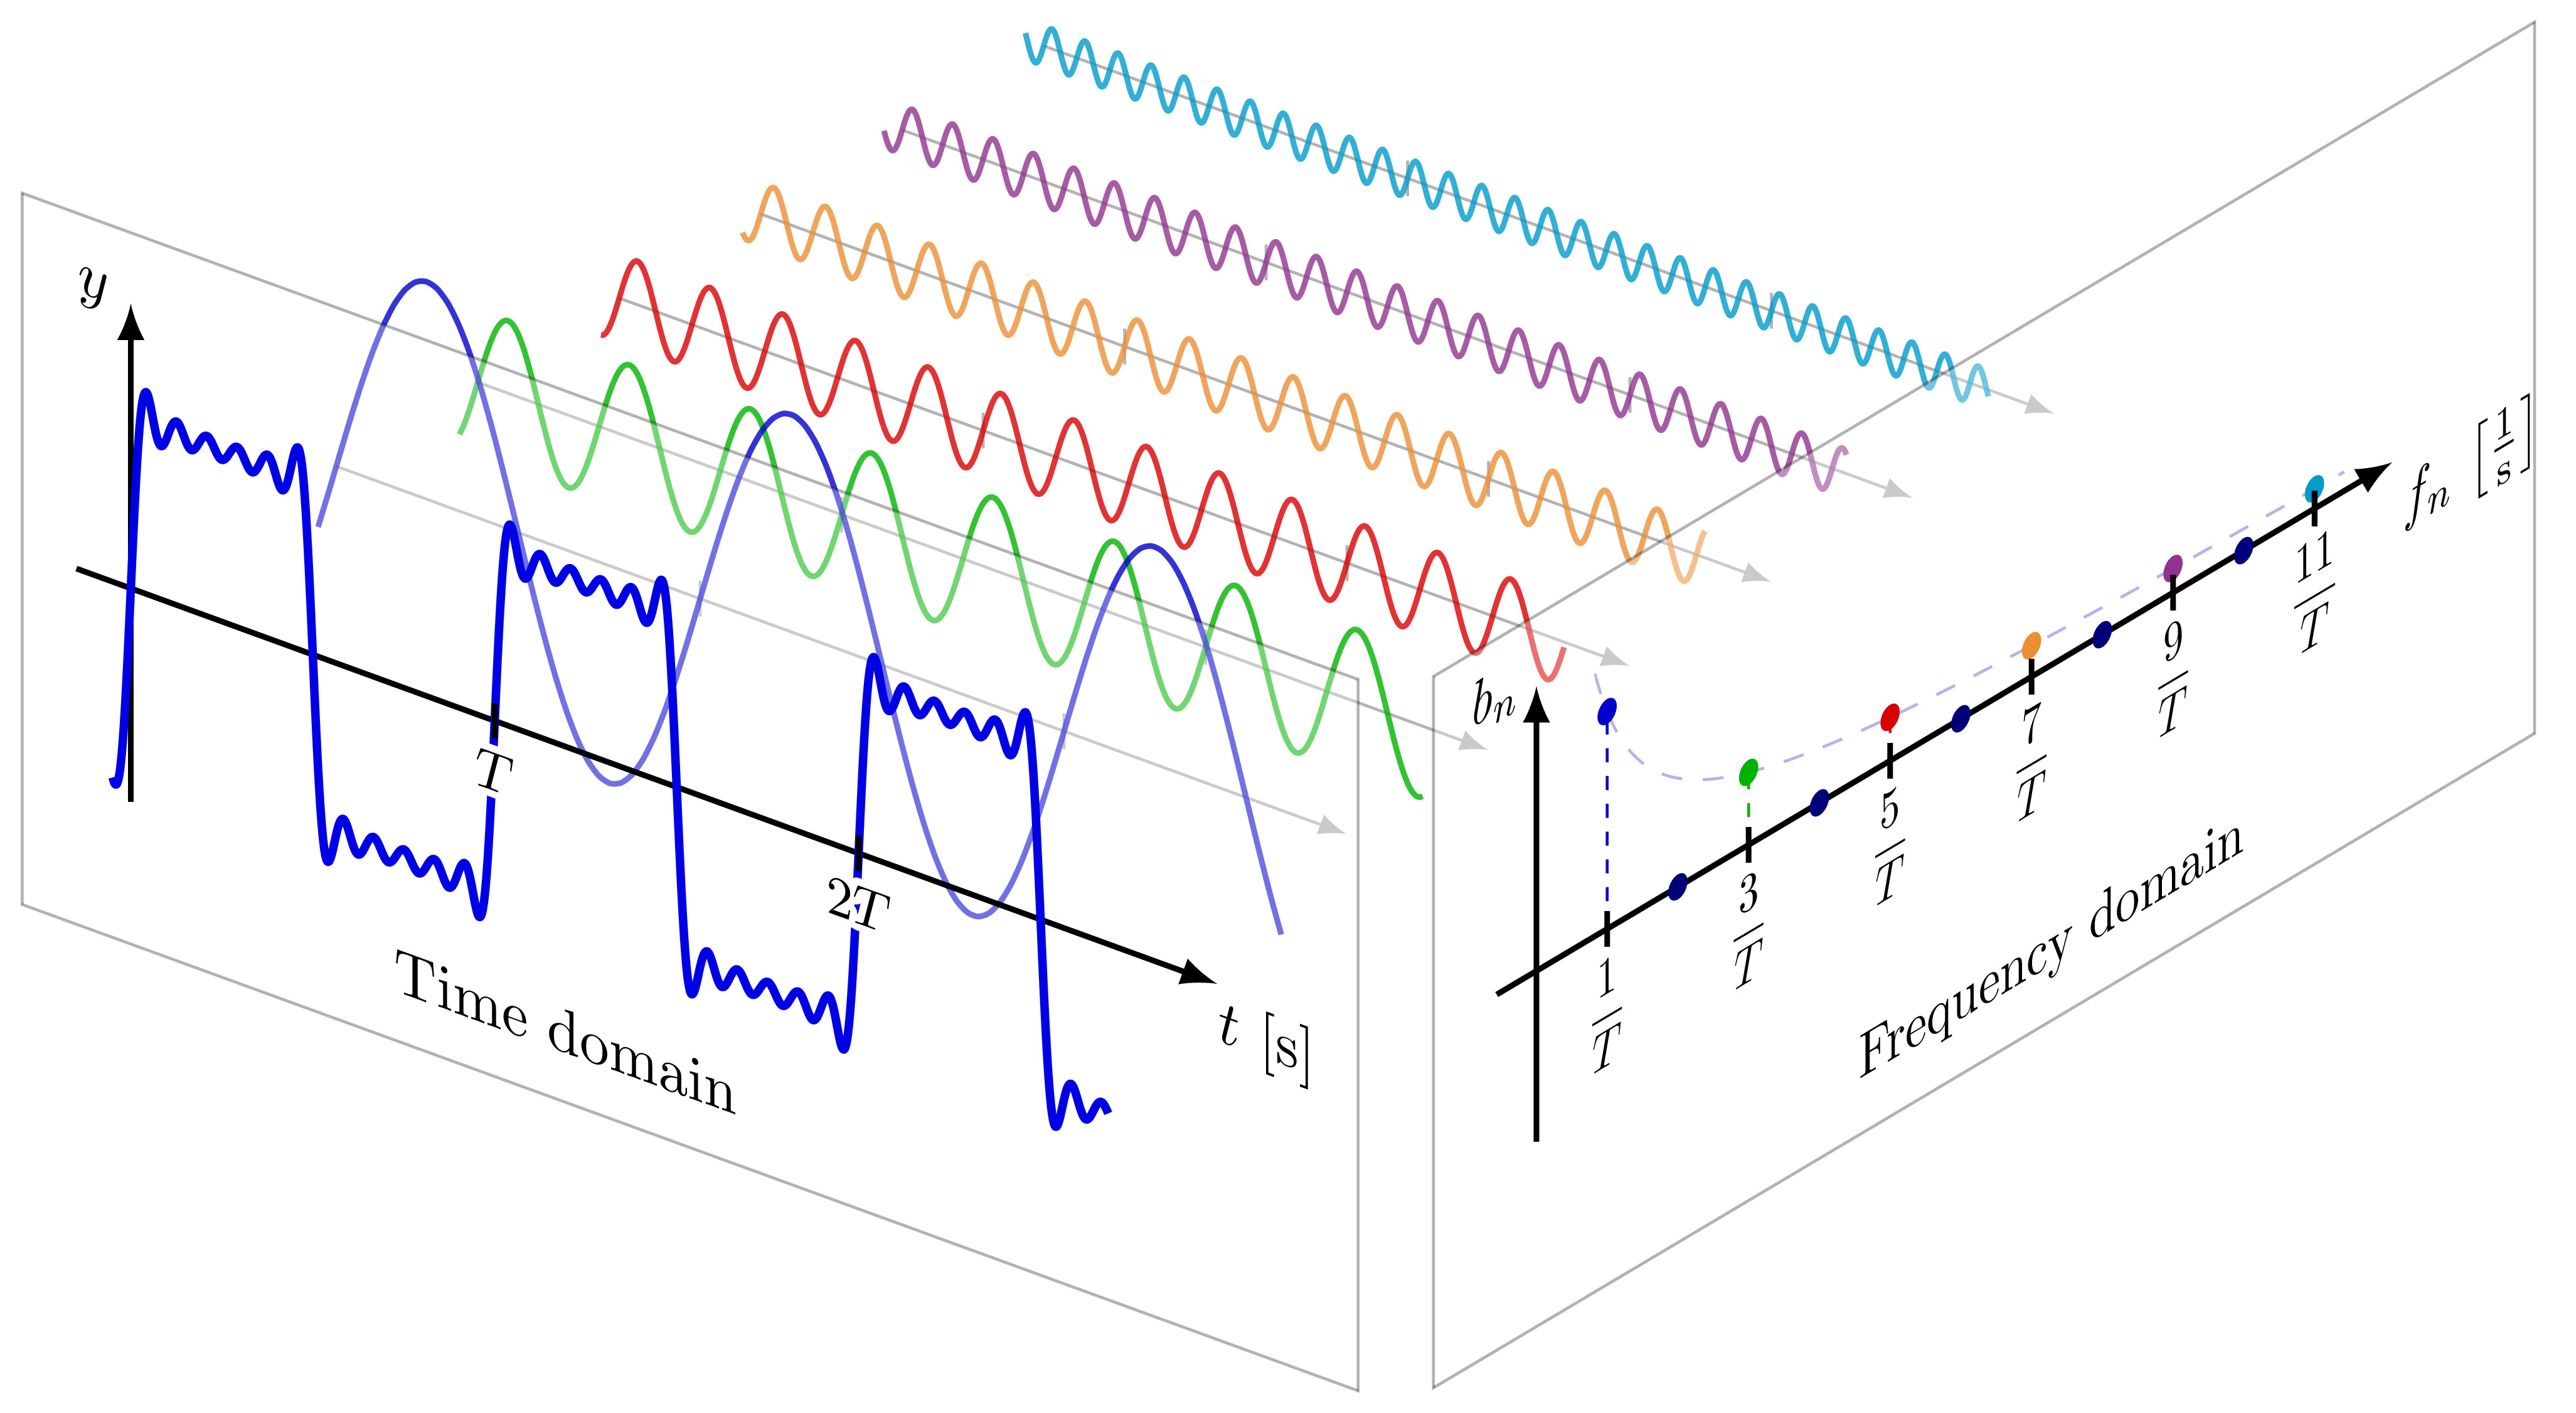
\includegraphics[width=0.6\linewidth]{Images/fourier_transform.jpeg}
    \caption{Representation of a time-domain signal decomposed into multiple signals of different frequencies.}
    \label{fig:time_domain_decomp}
\end{figure}

The Fourier transform, $\hat{f}(\omega)$, of a function $f(t)$ is defined mathematically as:

\begin{equation}
    \hat{f}(\omega) = \int_{-\infty}^{\infty} f(t) e^{-i\omega t} \, dt
\end{equation}

\section{Fast Fourier Transform in General}
The Fast Fourier Transform (FFT) is an efficient algorithm used to compute the Discrete Fourier Transform (DFT) of a sequence, which transforms a signal from the time domain into the frequency domain. This means it breaks down a complex signal into its constituent sinusoidal components, frequencies and their amplitudes, making it easier to analyze patterns such as pitch in audio, frequencies in communications, or periodicities in data. The FFT drastically reduces the computational complexity of DFT from $O(N^2)$ to $O(N\log(N))$ by cleverly reusing calculations through a divide-and-conquer approach. This algorithm is ideal for real-life applications like audio processing, image analysis, wireless communication, and other biomedical and industrial applications.

The most common FFT algorithm is the \textbf{Cooley-Tukey} algorithm~\cite{cooley1965}, which is widely used due to its simplicity and efficiency. It works best when the input size $N$ is a power of 2. The most common versions of the algorithm are:

\begin{itemize}
    \item \textbf{Radix-2}: The most basic and common version. Splits the DFT into two halves (even and odd indices) at each stage. Requires $N$ to be a power of 2.
    \item \textbf{Radix-4}: More efficient than Radix-2 when $N$ is a power of 4. Reduces the number of multiplications compared to Radix-2 by grouping four elements at a time.
    \item \textbf{Split-Radix}: This combines both Radix-2 and Radix-4 versions in order to improve computational efficiency.
\end{itemize}

\begin{figure}[H]
    \centering
    
    % Top row: Radix-2 and Radix-4
    \begin{subfigure}[t]{0.48\linewidth}
        \centering
        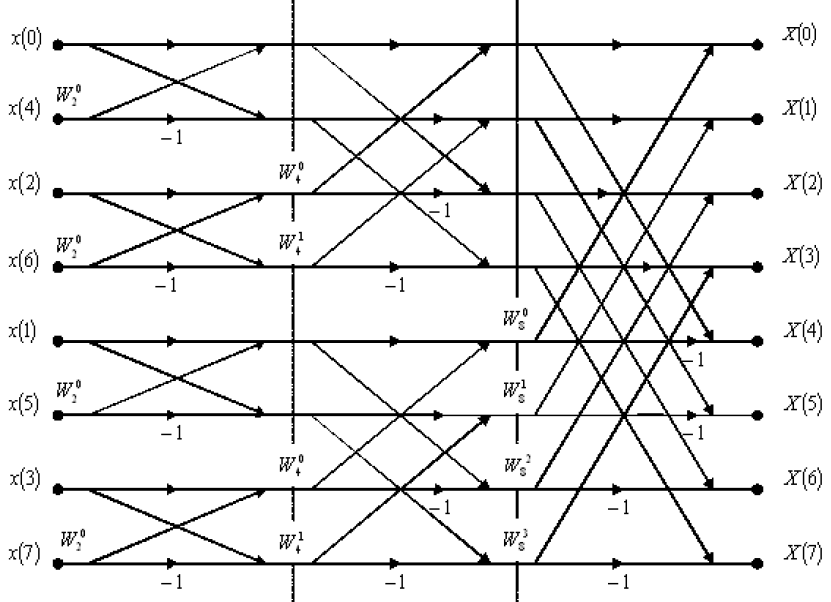
\includegraphics[width=\linewidth]{Images/r2.png}
        \caption{Radix-2 Dataflow}
        \label{fig:radix2_dataflow}
    \end{subfigure}
    \hfill
    \begin{subfigure}[t]{0.48\linewidth}
        \centering
        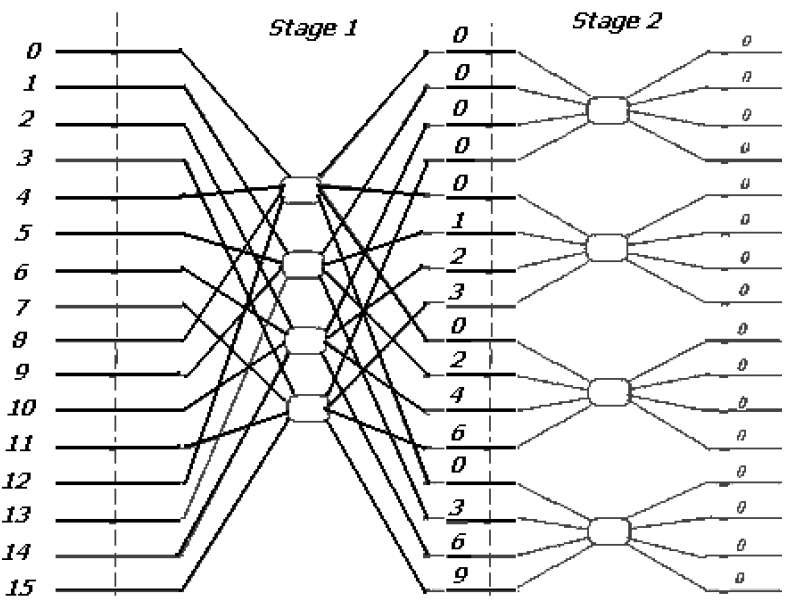
\includegraphics[width=\linewidth]{Images/r4.png}
        \caption{Radix-4 Dataflow}
        \label{fig:radix4_dataflow}
    \end{subfigure}
    
    \vspace{1em} % Adds a little space between the rows
    
    % Bottom row: Third image
    \begin{subfigure}[t]{\linewidth}
        \centering
        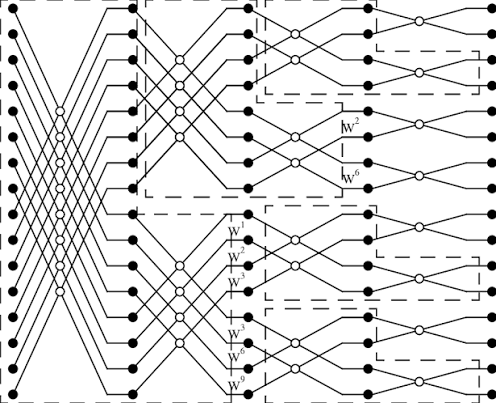
\includegraphics[width=0.6\linewidth]{Images/r_s.png}
        \caption{Split-Radix Dataflow}
        \label{fig:r_s_dataflow}
    \end{subfigure}
    
    % Main caption and label for the entire figure
    \caption{Comparison of Radix-2, Radix-4 and Split-Radix dataflow structures.}
    \label{fig:FFT_dataflows}
\end{figure}

\section{FFT Decomposition}
\subsection{Radix-2}

Given a sequence $x[n]$ of length $N$, the Discrete Fourier Transform (DFT) is defined as~\cite{oppenheim2010}:
\begin{equation}
    X[k] = \sum_{n=0}^{N-1} x[n] \cdot W_N^{kn}, \quad \text{where } W_N = e^{-j\frac{2\pi}{N}}
\end{equation}
Here, $W_N$ represents the \textbf{twiddle factor}. The primary advantage of the FFT algorithm is its ability to reorganize this summation, thereby drastically reducing the overall computational complexity.

By separating the input data $x[n]$ into even-indexed ($e[n] = x[2n]$) and odd-indexed ($o[n] = x[2n+1]$) elements, the DFT can be expressed as:
\begin{equation}
    X[k] = \sum_{n=0}^{N/2 - 1} x[2n] \cdot W_N^{k \cdot 2n} + \sum_{n=0}^{N/2 - 1} x[2n+1] \cdot W_N^{k \cdot (2n+1)}
\end{equation}
Applying the substitution $W_N^{2kn} = W_{N/2}^{kn}$, we can factor the equation into two smaller transforms:
\begin{equation}
    X[k] = \underbrace{\sum_{n=0}^{N/2 - 1} e[n] \cdot W_{N/2}^{kn}}_{\text{Even terms } (E[k])} + W_N^k \cdot \underbrace{\sum_{n=0}^{N/2 - 1} o[n] \cdot W_{N/2}^{kn}}_{\text{Odd terms } (O[k])}
\end{equation}
Let $E[k]$ and $O[k]$ represent the DFTs of the even and odd sequences, respectively. This reduces the main equation to:
\begin{equation}
    X[k] = E[k] + W_N^k \cdot O[k]
\end{equation}
Exploiting the $N$-periodicity of the DFT, the complete range for $k = 0, 1, \dots, N-1$ is evaluated using the standard \textbf{butterfly operation}:
\begin{align}
    X[k] &= E[k] + W_N^k \cdot O[k] \\
    X\left[k + \frac{N}{2}\right] &= E[k] - W_N^k \cdot O[k]
\end{align}
for $k = 0, 1, \dots, N/2 - 1$. For an input sequence where $N = 2^m$, this algorithm completes the transform in $m = \log_2(N)$ stages by recursively applying these butterfly operations.

\begin{figure}[H]
    \centering
    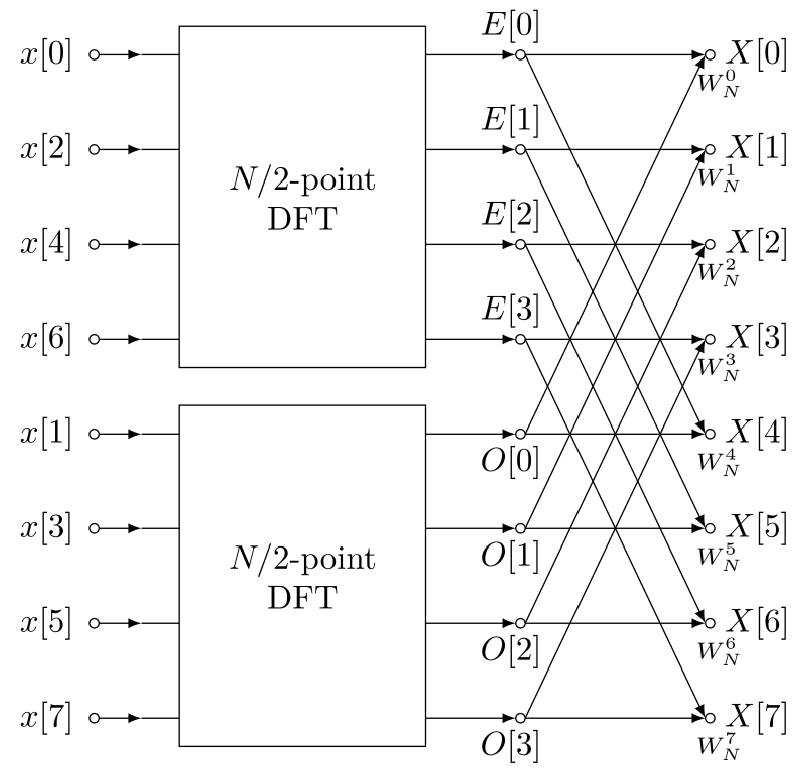
\includegraphics[width=0.4\textwidth]{Images/fft_rec.png} 
    \caption{Recursive logic of the Radix-2 FFT, demonstrating the combination of even and odd sequences from previous stages.}
    \label{fig:radix2_rec}
\end{figure}

\subsection{Radix-4}

The Radix-4 FFT builds upon the fundamental principles of Radix-2 by partitioning the DFT into \textbf{four smaller DFTs}. This requires the input sequence length $N$ to be a power of 4 (i.e., $N=4^m$).

The input sequence $x[n]$ is divided into four interleaved subsequences:
\begin{align}
    x_0[n] &= x[4n], & x_1[n] &= x[4n+1], \nonumber \\
    x_2[n] &= x[4n+2], & x_3[n] &= x[4n+3]
\end{align}
Expanding the DFT with these subsequences yields:
\begin{equation}
    X[k] = \sum_{n=0}^{N/4-1} \left[ 
    x[4n] + x[4n+1] W_N^k + x[4n+2] W_N^{2k} + x[4n+3] W_N^{3k}
    \right] W_{N/4}^{kn}
\end{equation}
This equation effectively acts as a linear combination of four $N/4$-point DFTs, denoted as $X_0, X_1, X_2, \text{ and } X_3$:
\begin{equation}
    X[k] = X_0[k] + W_N^k X_1[k] + W_N^{2k} X_2[k] + W_N^{3k} X_3[k]
\end{equation}
To streamline the 4-point butterfly calculation, we define four intermediate variables:
\begin{equation}
    A = X_0[k], \quad B = W_N^k X_1[k], \quad C = W_N^{2k} X_2[k], \quad D = W_N^{3k} X_3[k]
\end{equation}
The resulting butterfly outputs are computed as follows:
\begin{align}
    X[k] &= A + B + C + D \\
    X\left[k + \frac{N}{4}\right] &= A - jB - C + jD \\
    X\left[k + \frac{N}{2}\right] &= A - B + C - D \\
    X\left[k + \frac{3N}{4}\right] &= A + jB - C - jD
\end{align}
By leveraging additional symmetries, the Radix-4 algorithm lowers the total number of stages to $\log_4(N)$. This significantly reduces the multiplication count compared to Radix-2, making it highly efficient for hardware implementations when applicable.

\subsection{Split-Radix}

The \textbf{Split-Radix FFT (SRFFT)} elegantly combines the structures of Radix-2 and Radix-4 to achieve superior computational efficiency. It relies on the mathematical observation that the even-indexed terms of the DFT are best computed using a Radix-2 approach, while the odd-indexed terms are more efficiently handled using a Radix-4 approach. This method yields the lowest number of arithmetic operations for power-of-two FFTs.

The standard DFT is decomposed by applying a Radix-2 split to the even indices, and a Radix-4 split to the odd indices:
\begin{equation}
    X[k] = \sum_{n=0}^{N/2-1} x[2n] W_{N/2}^{kn} + \sum_{n=0}^{N/4-1} x[4n+1] W_N^{k(4n+1)} + \sum_{n=0}^{N/4-1} x[4n+3] W_N^{k(4n+3)}
\end{equation}
By factoring out the twiddle factors for the odd terms, the equation simplifies to:
\begin{equation}
    X[k] = \sum_{n=0}^{N/2-1} x[2n] W_{N/2}^{kn} + W_N^k \sum_{n=0}^{N/4-1} x[4n+1] W_{N/4}^{kn} + W_N^{3k} \sum_{n=0}^{N/4-1} x[4n+3] W_{N/4}^{kn}
\end{equation}
Let $E[k]$ be the $N/2$-point DFT of the even elements, and let $O_1[k]$ and $O_3[k]$ represent the $N/4$-point DFTs of the two interleaved odd sequences. The Split-Radix butterfly operation computes four outputs simultaneously using an L-shaped structure:
\begin{align}
    X[k] &= E[k] + \left( W_N^k O_1[k] + W_N^{3k} O_3[k] \right) \\
    X\left[k + \frac{N}{2}\right] &= E[k] - \left( W_N^k O_1[k] + W_N^{3k} O_3[k] \right) \\
    X\left[k + \frac{N}{4}\right] &= E\left[k + \frac{N}{4}\right] - j \left( W_N^k O_1[k] - W_N^{3k} O_3[k] \right) \\
    X\left[k + \frac{3N}{4}\right] &= E\left[k + \frac{N}{4}\right] + j \left( W_N^k O_1[k] - W_N^{3k} O_3[k] \right)
\end{align}
Because it selectively applies the most efficient decomposition step at each stage, the Split-Radix algorithm requires up to one third fewer multiplications than standard Radix-2~\cite{duhamel1984}, without placing the strict $N=4^m$ size restriction required by pure Radix-4.

\section{Unrolled and Single-Path Delay Feedback Approaches}
There are different approaches to designing the FFT algorithm in hardware. The most intuitive method is the unrolled architecture, which exploits inherent parallelism by unrolling the entire computation. Each butterfly operation is assigned a dedicated hardware unit, resulting in a fully unrolled design where all butterfly computations are executed concurrently. This method is very demanding in resources, especially for smaller FPGAs. Furthermore, it requires a very high data bandwidth, as a 256-point FFT would typically require access to 256 data points in the same clock cycle. For example, if each complex sample is 32 bits (16bits real and 16bits imaginary) long and the FFT operates at 100 MHz, the system requires a continuous bandwidth of 819.2 Gbps to run without stalling.

\begin{figure}[htbp]
    \centering
    \begin{subfigure}[t]{0.48\linewidth}
        \centering
        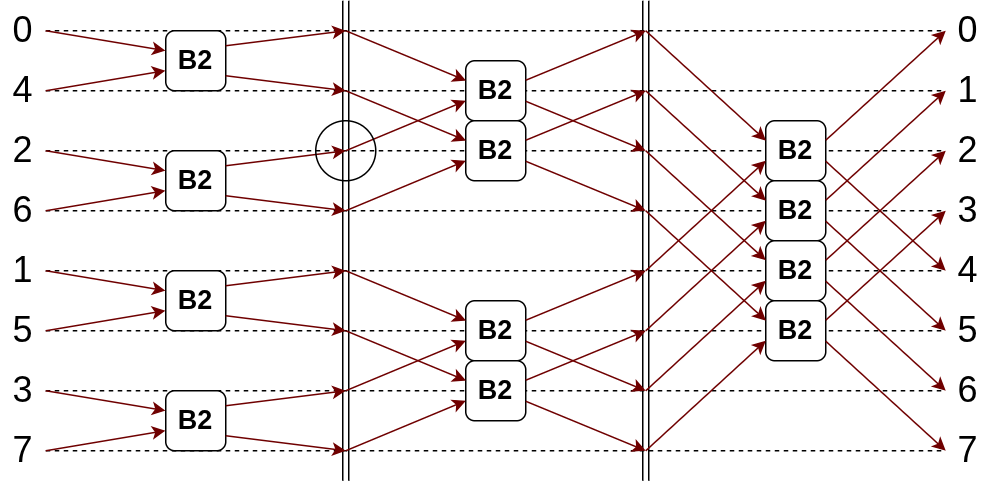
\includegraphics[width=\linewidth]{Images/r2_.png}
        \caption{Structure/dataflow of the Radix-2 unrolled algorithm (B2 = Butterfly 2).}
        \label{fig:radix2_unrolled}
    \end{subfigure}
    \hfill
    \begin{subfigure}[t]{0.48\linewidth}
        \centering
        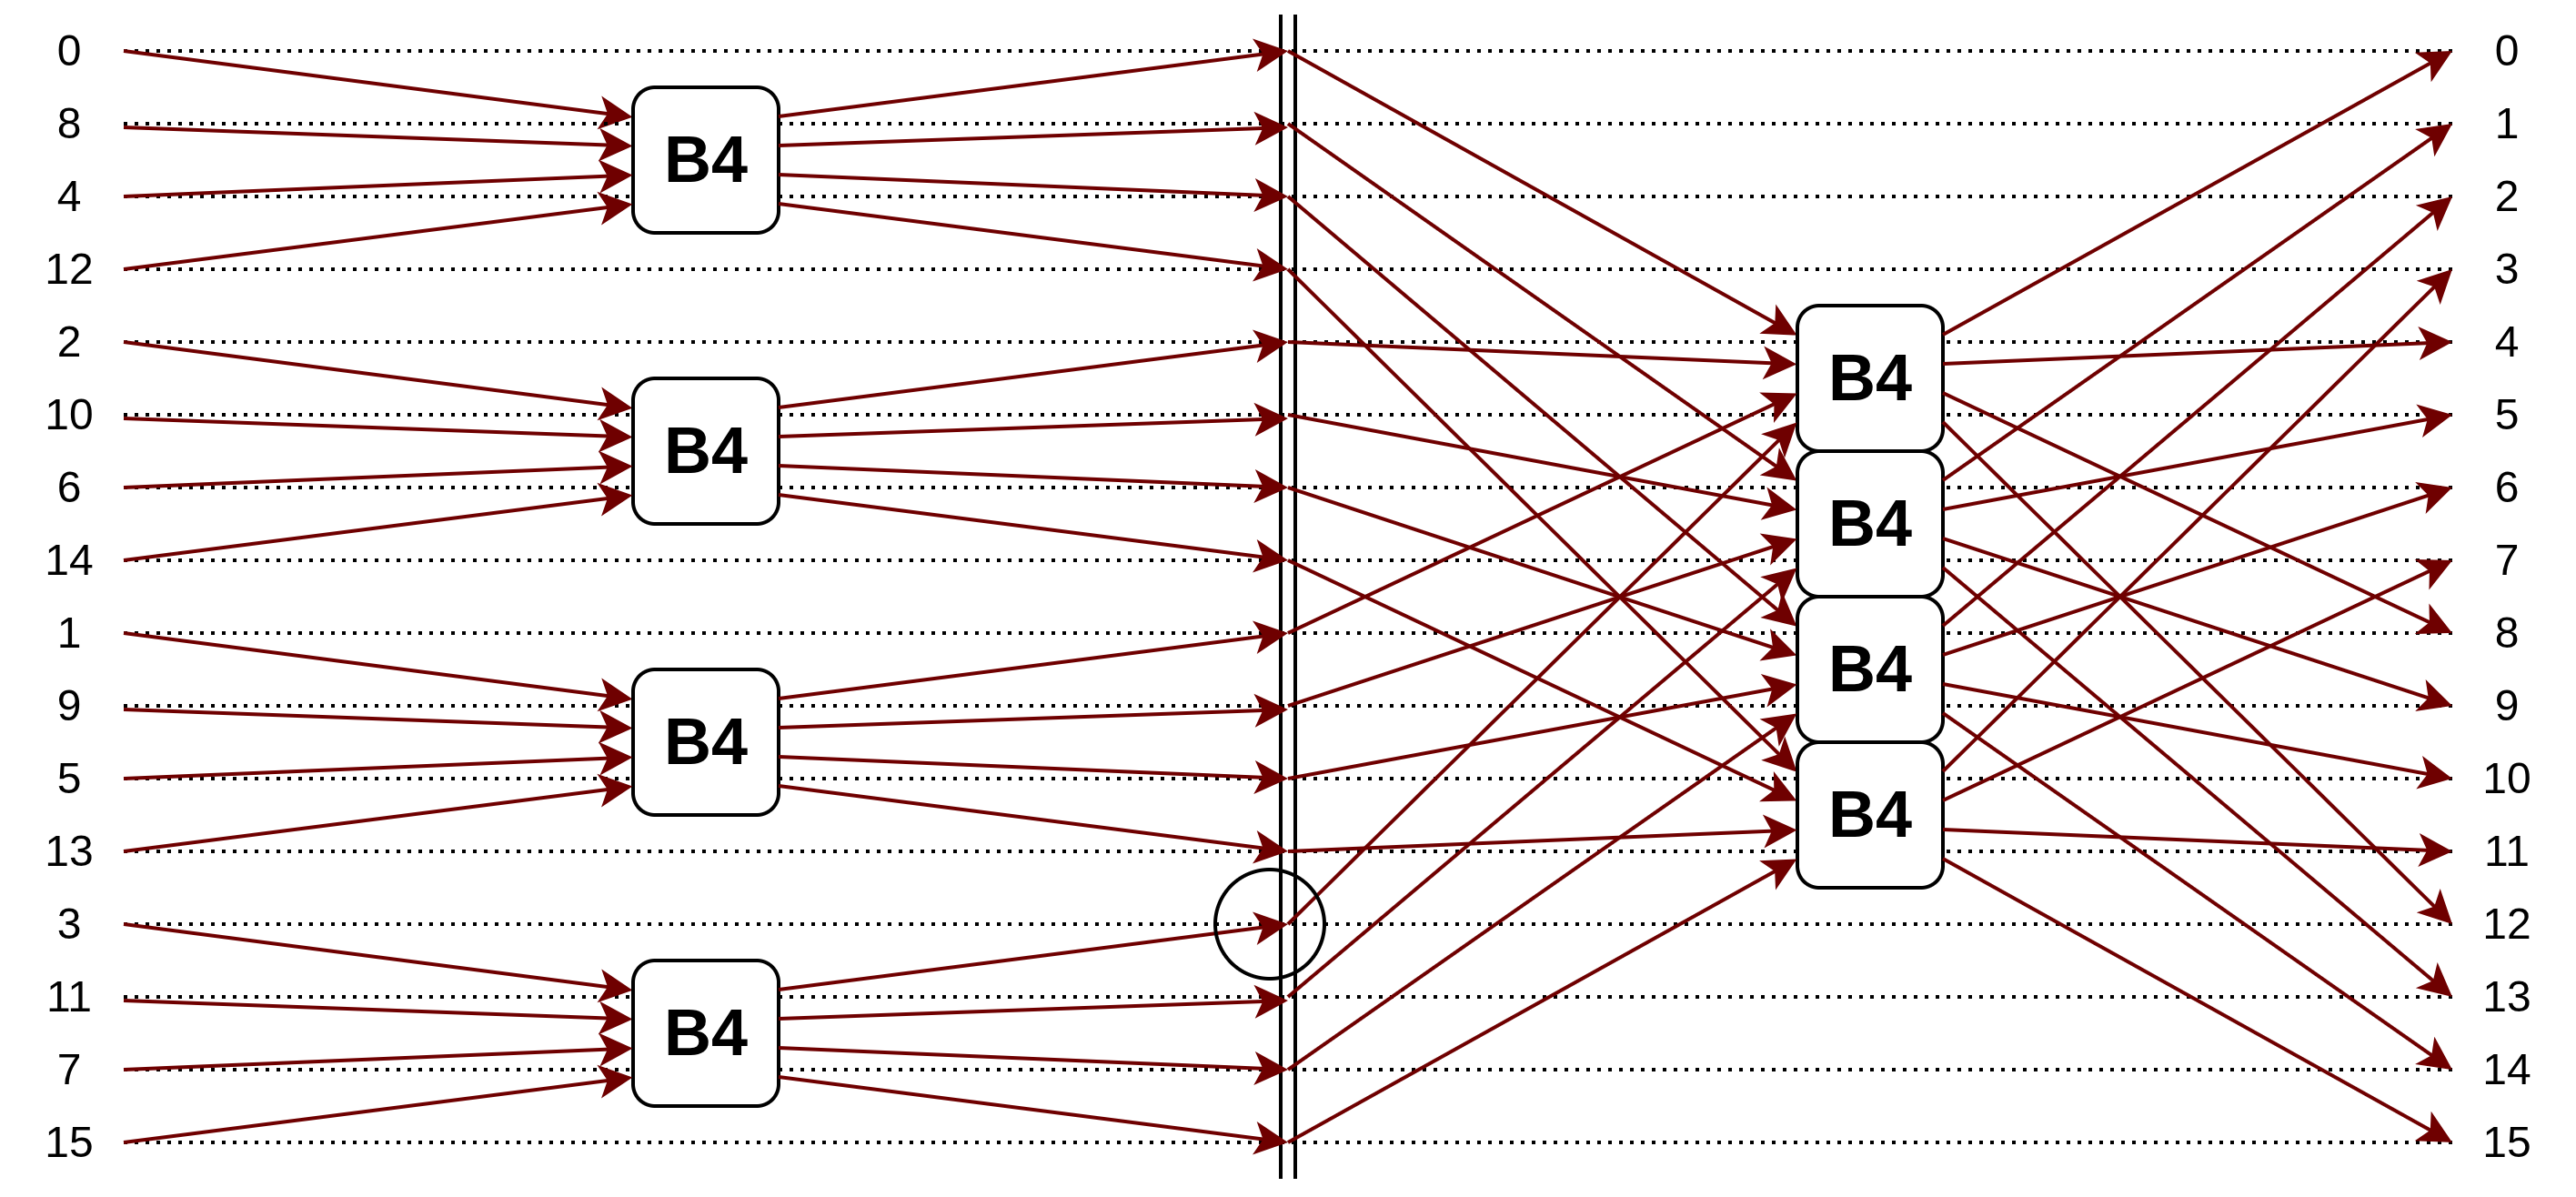
\includegraphics[width=\linewidth]{Images/r4.drawio_1.png}
        \caption{Structure/dataflow of the Radix-4 unrolled algorithm (B4 = Butterfly 4).}
        \label{fig:radix4_unrolled}
    \end{subfigure}
    \caption{Comparison of unrolled architectures.}
\end{figure}

A highly resource-efficient alternative allocates only a single butterfly unit per FFT stage, employing delay lines or memory buffers to schedule the incoming data streams for computation. This approach is known as Single-Path Delay Feedback (SDF) when the datapath processes a single continuous stream of samples, or Multi-Path Delay Feedback (MDF) when it processes multiple parallel samples. Due to its optimal balance of high throughput and minimal hardware footprint, SDF remains the most widely adopted architecture for modern FFT cores. 

\begin{figure}[H]
    \centering
    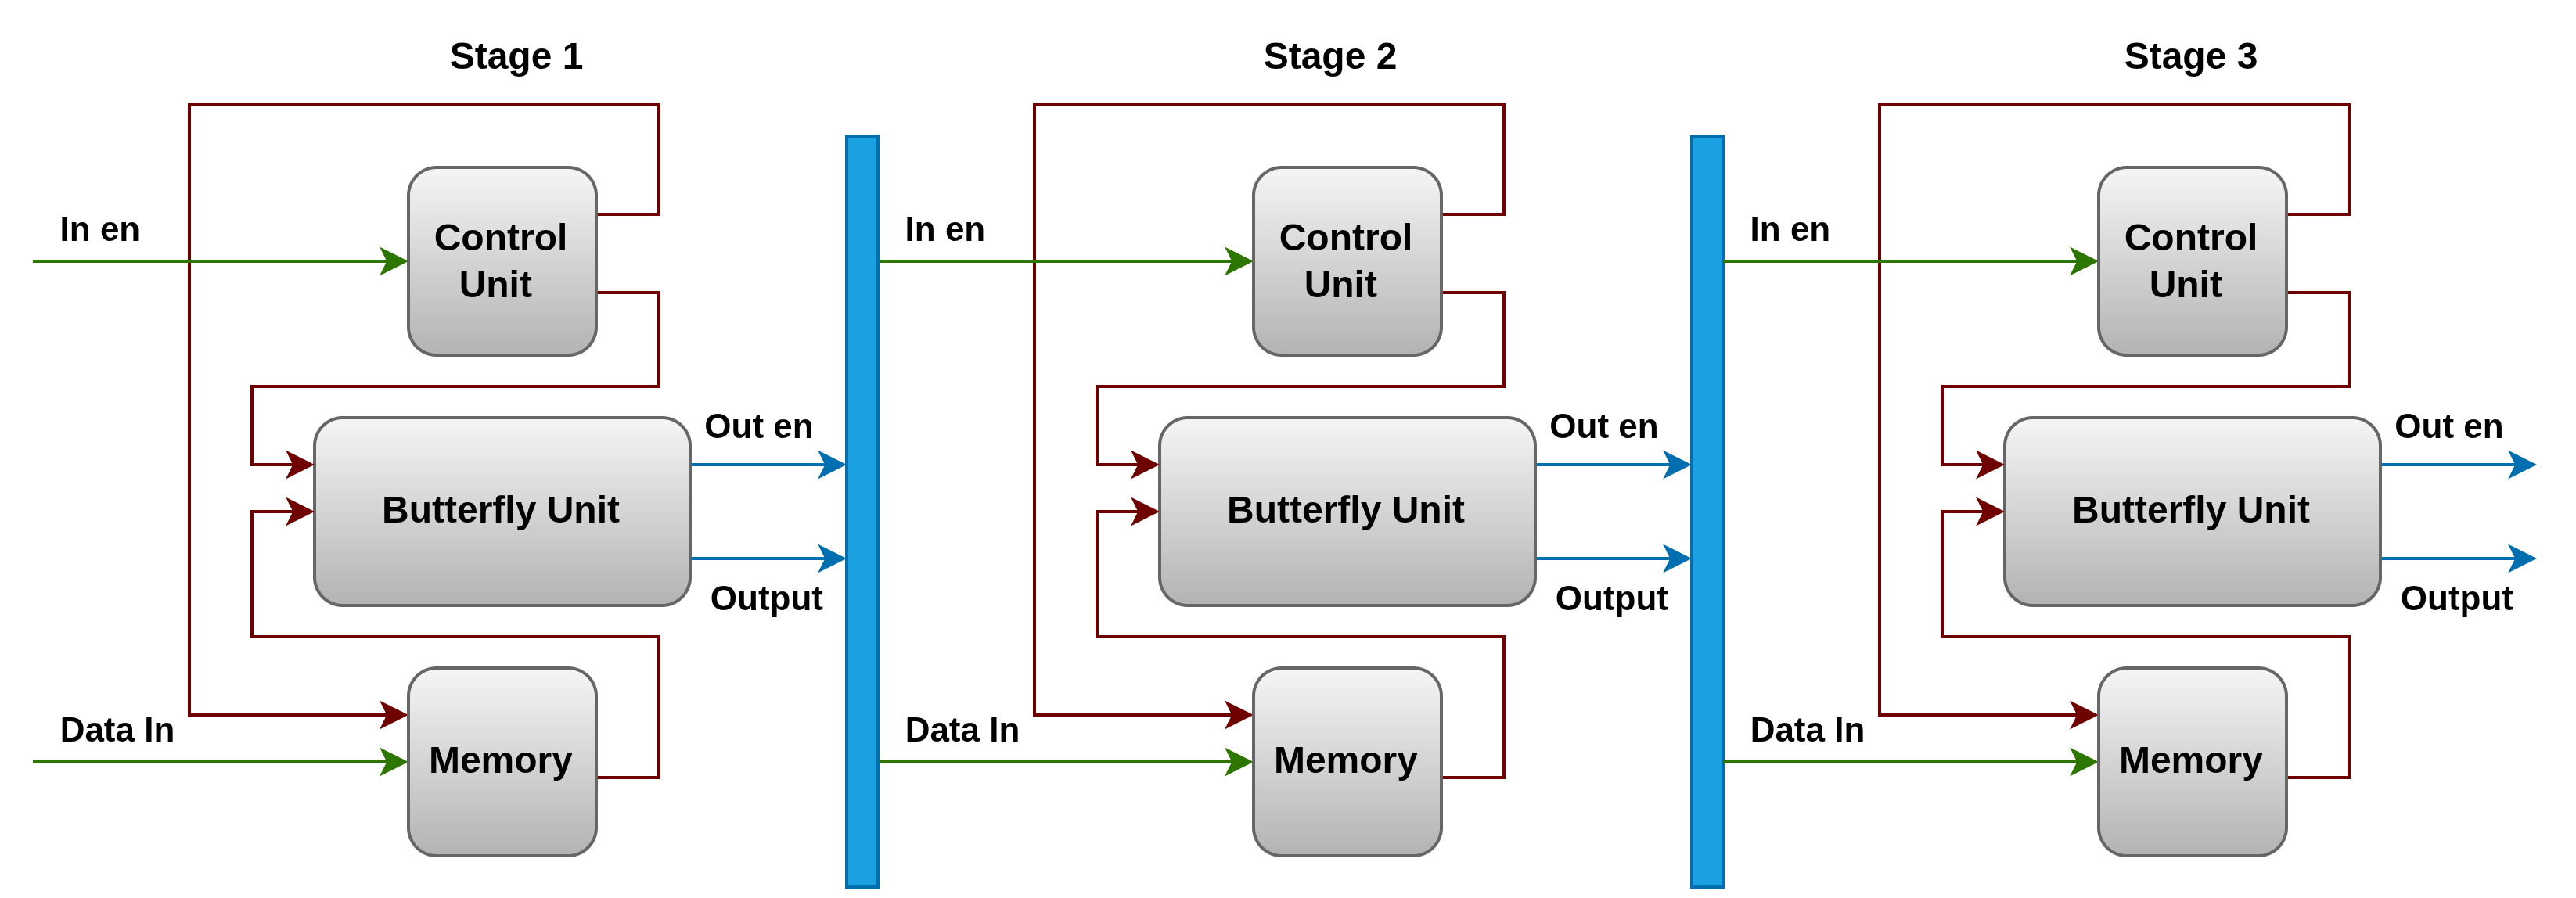
\includegraphics[width=1\linewidth]{Images/SDF_unit.png}
    \caption{Simplified diagram of the SDF units discussed in this chapter.}
    \label{fig:sdf_unit_intro}
\end{figure}

\section{Fixed-Point Arithmetic and Quantization Noise}
In hardware implementations of the FFT, floating-point arithmetic is typically avoided due to its high resource consumption and latency. Instead, signals and twiddle factors are represented using fixed-point formats, such as the Q format. For instance, a 32-bit data path might utilize a Q1.15 effective scaling, where a value of 1.0 corresponds to the integer 32767. The mathematical representation of this quantization scales a continuous signal $x(t)$ by a factor of $2^{W-1}-1$, where $W$ is the word length.  

Because fixed-point variables have finite precision, rounding or truncation occurs after mathematical operations, particularly after complex multiplications with twiddle factors. This introduces a small amount of error known as quantization noise. This error accumulates with every successive stage of the FFT.
The degradation is evaluated using the Signal-to-Quantization-Noise Ratio (SQNR), which compares the power of the original signal to the power of the quantization noise.

\begin{figure}[htbp]
    \centering
    \vspace{1em}
    
    % Power equation
    $\displaystyle P_{x^\nu} = 10\log_{10} \left( \frac{1}{N} \sum_{n=0}^{N-1} |x[n]|^2 \right)$
    
    \vspace{1.5em}
    
    % SQNR equation
    $\displaystyle \text{SQNR}|_{dB} = P_{x^\nu} + 6.02\nu + 4.77$
    
    \vspace{1em}
    \caption{Formulas for the signal power and Signal-to-Quantization-Noise Ratio (SQNR). $P_{x^\nu}$ represents the average power of the input signal. $\nu$ represents the number of bits (resolution).}
    \label{fig:sqnr_and_power}
\end{figure}

To determine the absolute maximum SQNR for a given bit depth, we assume a full-scale square input wave, which provides a normalized linear average power of 1 ($10\log_{10}(1) = 0$ dB). Consequently, for a 16-bit resolution, the maximum achievable SQNR is 101.09 dB. Table \ref{tab:max_sqnr} demonstrates the theoretical maximum SQNR limits across common hardware bit depths.

\begin{table}[htbp]
    \centering
    \caption{Maximum theoretical SQNR for various hardware bit depths (assuming full-scale square wave input).}
    \vspace{0.5em}
    \begin{tabular}{|c|c|}
        \hline
        \textbf{Resolution ($\nu$ bits)} & \textbf{Maximum SQNR (dB)} \\
        \hline
        8 & 52.93 \\
        12 & 77.01 \\
        16 & 101.09 \\
        \hline
    \end{tabular}
    \label{tab:max_sqnr}
\end{table}

\section{Custom Multipliers}
This thesis implements two distinct custom multiplier architectures: a generic carry-save array multiplier for general arithmetic operations and a specialized computation-sharing multiplier (CSHM) optimized for signal processing workloads.

\subsection{Carry-Save Array Multiplier}

A Carry-Save Array Multiplier (CSAM) accelerates arithmetic by eliminating the intermediate carry-propagation delays found in standard array multipliers. The operation consists of three main stages:

\begin{enumerate}
    \item \textbf{Partial Product Generation:} A matrix of partial products is created using logical AND gates between the multiplicand and multiplier bits.
    \item \textbf{Carry-Save Reduction:} Instead of rippling carries horizontally across rows, Carry-Save Adders (CSAs) are used. Each CSA passes independent sum and carry bits diagonally down to the next row, keeping the intermediate results as two unmerged vectors.
    \item \textbf{Final Addition:} A traditional carry-propagate adder is used only at the very last stage to merge the final sum and carry vectors into the resolved product.
\end{enumerate}

By breaking the horizontal carry chain during intermediate steps, the CSAM reduces the critical path delay while maintaining a highly regular hardware structure suitable for FPGAs.

\begin{figure}[H]
    \centering
    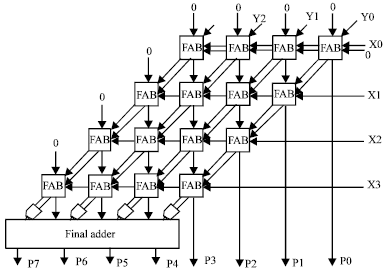
\includegraphics[width=0.6\linewidth]{Images/Carry-Save-Multiplier.png}
    \caption{Top diagram of the Carry-Save Array Multiplier discussed in this chapter}
    \label{fig:Carry-Save Mult}
\end{figure}

\subsection{Computation-Sharing Hardware Multiplier (CSHM)}

The Computation-Sharing Hardware Multiplier (CSHM) minimizes hardware logic by identifying and reusing redundant partial products. It is highly efficient for signal processing tasks where a single input data stream is multiplied by various coefficients.

\begin{itemize}
    \item \textbf{Alphabets and Sets:} CSHM simplifies multiplication by decomposing coefficients into a small set of recurring factor patterns, known as an \textit{alphabet}. A common basis set consists of small odd integers, such as $\{1, 3, 5, 7\}$. The architecture precomputes the multiplicand against this limited set of values.
    \item \textbf{Addition and Assembly:} Generating the initial alphabet set requires minimal hardware (e.g., $3x$ is computed as $2x + x$, requiring just one shift and one adder). The final multiplication product is then reconstructed by selecting, shifting, and adding these precomputed set values together. This computation-sharing approach drastically reduces the total number of resources and latency required compared to a classical multiplier.
\end{itemize}

\begin{figure}[H]
    \centering
    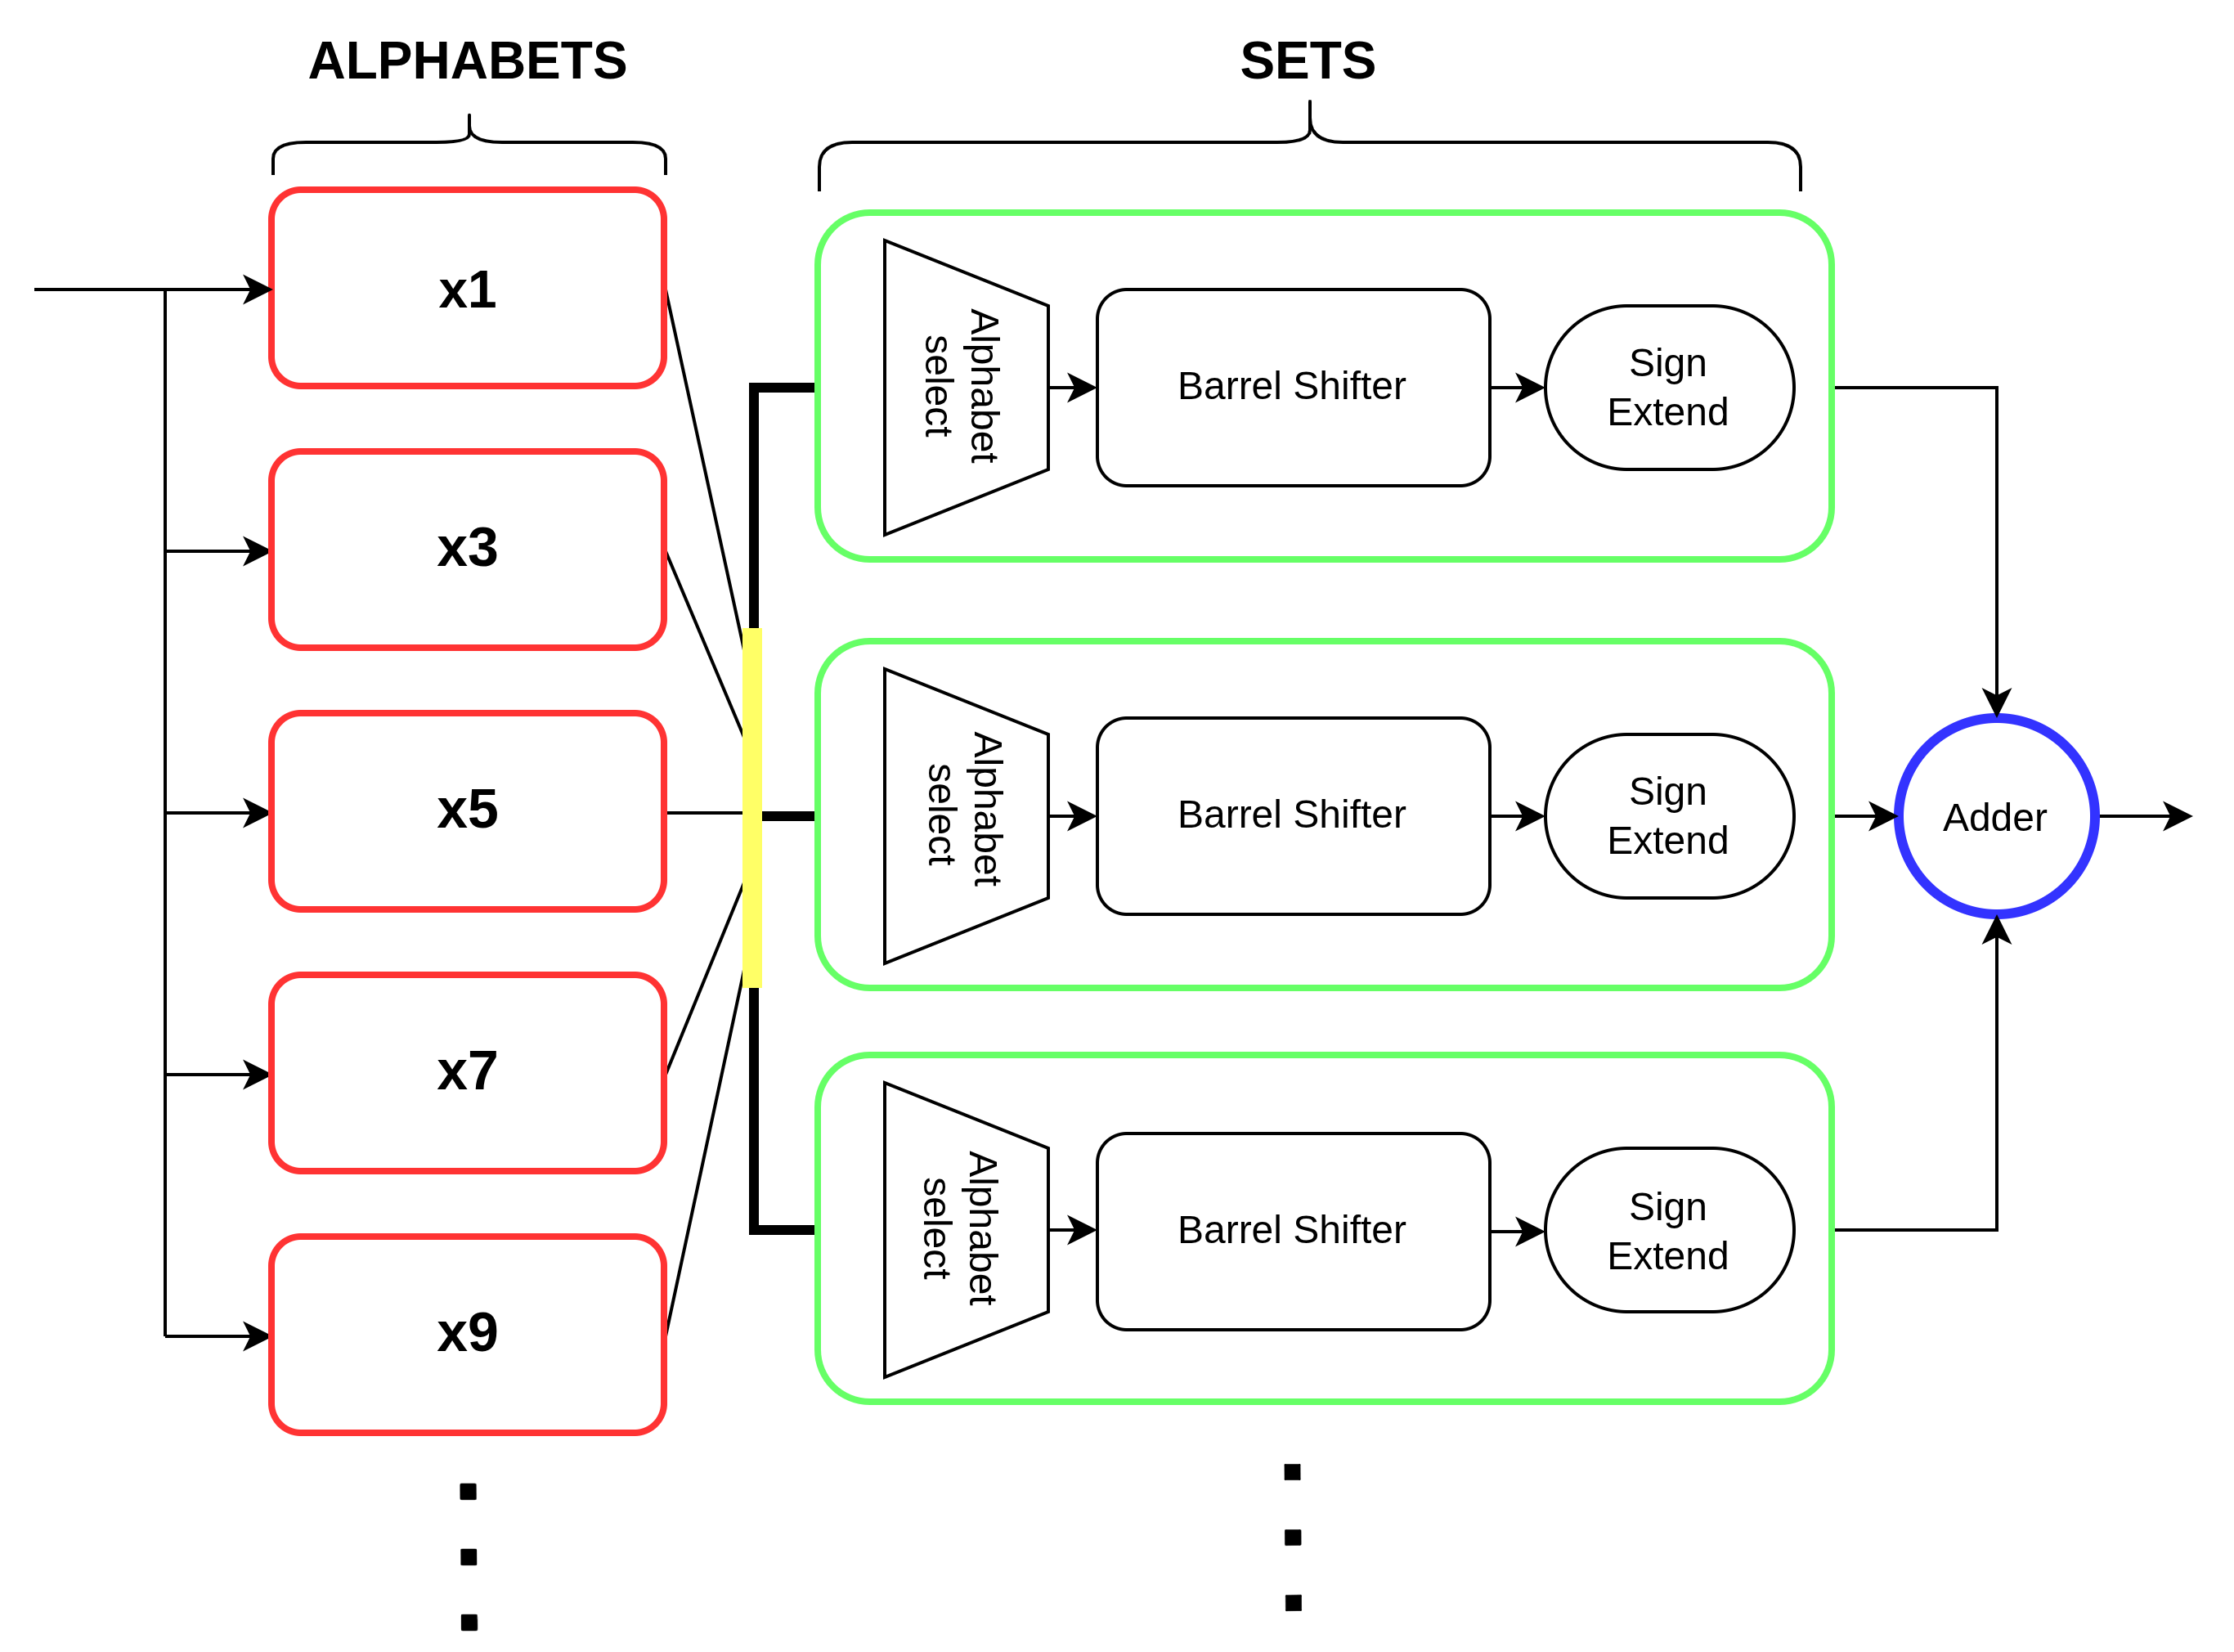
\includegraphics[width=0.8\linewidth]{Images/CSHM_gen.drawio.png}
    \caption{Top diagram of the CSHM Multiplier discussed in this chapter}
    \label{fig:Cshm general Unit}
\end{figure}

\begin{itemize}
    \item \textbf{Examples:}
    
        \textbf{Using a 2-Bit Set ($\{1, 3\}$):} Consider multiplying an input $x$ by the coefficient $27$ (binary $011011_2$). The coefficient is partitioned into 2-bit slices: $01_2$ (1), $10_2$ (2), and $11_2$ (3). The multiplication is reconstructed as $(1x \cdot 2^4) + (1x \cdot 2^3) + (3x \cdot 2^0)$. The hardware routes and shifts the precomputed $1x$ and $3x$ values, avoiding full multipliers.\\
        \textbf{Using a 3-Bit Set ($\{1, 3, 5, 7\}$):} Consider multiplying an input $x$ by the coefficient $45$ (binary $101101_2$). The coefficient is partitioned into 3-bit slices: $101_2$ (5) and $101_2$ (5). The multiplication is reconstructed as $(5x \cdot 2^3) + (5x \cdot 2^0)$. The hardware only needs to compute the partial product $5x$ once, sharing that computation for both halves of the coefficient.
\end{itemize}

\section{FPGA Hardware Resources}

Modern Field-Programmable Gate Arrays (FPGAs) provide dedicated architectural primitives to accelerate digital signal processing algorithms and manage data streams efficiently. The hardware implementation of the proposed FFT and custom multipliers relies heavily on three core resources:

\begin{itemize}
    \item \textbf{Digital Signal Processing (DSP) Blocks:} These are dedicated, hard-silicon arithmetic units embedded within the FPGA fabric (such as DSP48 slices in AMD/Xilinx architectures~\cite{ug479}). They are optimized to perform high-speed, wide-bit operations like multiply-accumulate (MAC) and pre-addition.
    
    \item \textbf{Block RAM (BRAM):} BRAMs are dedicated memory blocks~\cite{ug473} arranged in columns throughout the FPGA. They provide high-capacity, synchronous data storage and can be configured as single-port or dual-port memories.
    
    \item \textbf{Look-Up Table RAM (LUTRAM) / Distributed RAM:} LUTRAM is generated by the logic Look-Up Tables (LUTs) in the general logic fabric~\cite{ug473} to act as small memory elements. While it provides less capacity than a BRAM, LUTRAM is placed directly next to logic cells, making it efficient for implementing small memory structures.
\end{itemize}
    \chapter{Hardware Implementation of the Proposed Algorithms}
\label{Implementation}

\section{Introduction}
This chapter presents the detailed hardware architectures developed for each FFT algorithm. It provides an in-depth analysis of critical design choices, including Block RAM (BRAM) allocation, DSP block utilization, delay register configuration, and pipelining strategies. Finally, it evaluates how these architectural decisions directly impact overall hardware resource utilization and computational latency.

\section{Shared Architectural Elements}
Before examining each algorithm individually, it is necessary to outline the design choices that are universally applied across all three implementations. Specifically, these shared architectural elements include the generation of twiddle factors, datapath optimization  to minimize resource consumption, the application of different complex multipliers architectures and the datatypes used.

\subsection{Twiddle Factors}
Because the proposed hardware implementations are designed for FFTs of fixed sizes (although the underlying RTL is parameterizable, the synthesized modules target specific sizes), there is no need to compute twiddle factors dynamically at runtime. Calculating these rotational coefficients involves trigonometric operations that are computationally expensive and consume valuable FPGA logic resources. To optimize efficiency, all twiddle factors are precomputed at compile time and statically stored in on-chip memory.

Given that certain FFT architectures require simultaneous access to multiple twiddle factors, the choice of memory architecture is critical. The memory must provide sufficient read bandwidth to prevent stalling the datapath. To meet these high-throughput requirements, twiddle factors are implemented using read-only distributed memory (such as LUTRAM or dedicated flip-flops). This guarantees single-cycle, constant-time access, ensuring that the computational units can retrieve the required constants without delay.

For example, the Radix-4 algorithm requires three distinct twiddle factors simultaneously for each butterfly computation. Attempting to store these coefficients in BRAM would be highly inefficient and structurally limiting, as BRAM primitives are strictly restricted to dual-port (two-read) operations. In contrast, distributed read-only memory supports multi-port parallel reads and synthesizes very efficiently within the general FPGA logic fabric.

\begin{figure}[H]
    \centering
    \begin{subfigure}[t]{0.48\linewidth}
        \centering
        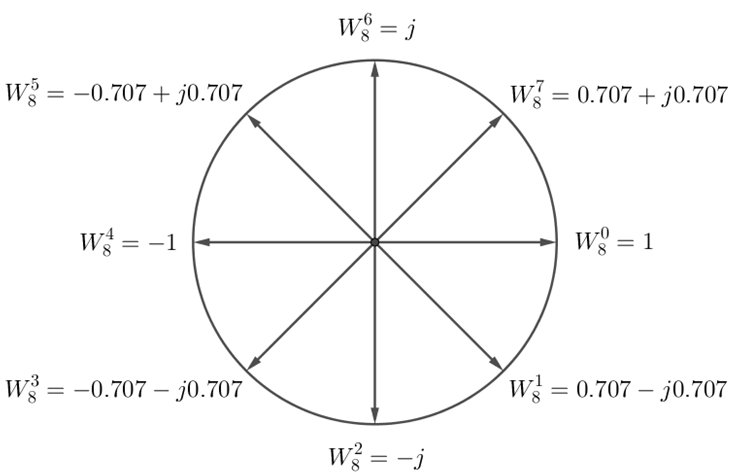
\includegraphics[width=\linewidth]{Images/cyrcle_2.png}
        \caption{Twiddle factors for N=8 represented on the unit circle.}
        \label{fig:twiddle_circle}
    \end{subfigure}
    \hfill
    \begin{subfigure}[t]{0.48\linewidth}
        \centering
        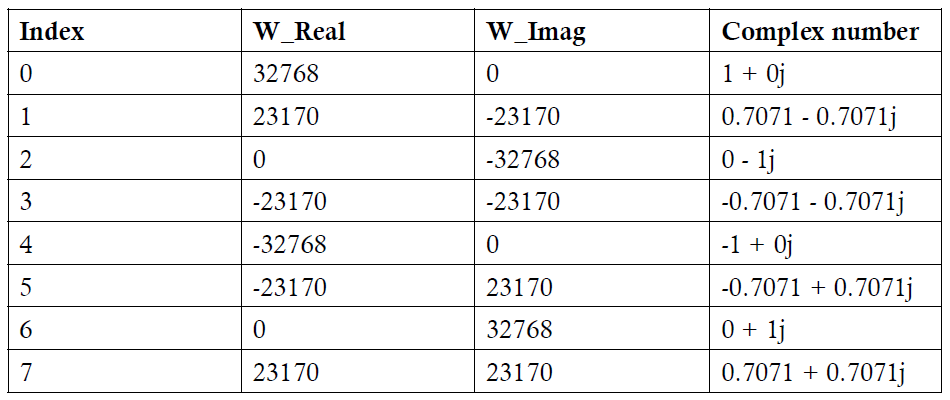
\includegraphics[width=\linewidth]{Images/tw.png}
        \caption{Twiddle values for N=8.}
        \label{fig:twiddle_values}
    \end{subfigure}
    \caption{Twiddle factor visualization.}
\end{figure}

The twiddle factors are generated by sampling the complex exponential function, $W_N = e^{-j\frac{2\pi}{N}}$, at $N$ discrete intervals, where $N$ represents the size of the FFT. These ideal floating-point values are subsequently quantized to match the target fixed-point resolution used in the hardware datapath.

The intuitive approach to storing twiddle factors would be to utilize a single, centralized memory shared across all FFT stages. However, this is architecturally impractical for a highly pipelined design. First, standard BRAM primitives lack the multi-port capabilities required for simultaneous multi-stage access. Second, implementing a centralized memory using read-only LUTRAMs would require extensive logic replication to achieve the necessary read bandwidth, completely defeating the purpose of a unified memory structure.Consequently, the design employs a distributed memory architecture, allocating a dedicated memory module to each individual FFT stage. However, because different stages require different subsets of the twiddle factors, duplicating the entire $N$-point coefficient array at every stage would be highly inefficient. To optimize resource utilization, a custom generation script was developed that mimics the algorithmic dataflow of the FFT. This script precomputes and generates customized, stage-specific memory modules that contain only the exact coefficients required for that particular stage, drastically minimizing the overall memory footprint.

\begin{table}[htbp]
    \centering
    \caption{Comparison of twiddle factor memory footprint between a naive duplicated storage approach and the proposed stage-specific optimized generation for an 8-stage Radix-2 FFT (DIT).}
    \vspace{0.5em}
    \begin{tabular}{|c|c|c|}
        \hline
        \textbf{FFT Stage} & \textbf{Naive Storage (Duplicated)} & \textbf{Optimized Storage} \\
        \hline
        Stage 1 & 128 & 1 \\
        Stage 2 & 128 & 2 \\
        Stage 3 & 128 & 4 \\
        Stage 4 & 128 & 8 \\
        Stage 5 & 128 & 16 \\
        Stage 6 & 128 & 32 \\
        Stage 7 & 128 & 64 \\
        Stage 8 & 128 & 128 \\
        \hline
        \textbf{Total Twiddle Factors} & \textbf{1024} & \textbf{255} \\
        \hline
    \end{tabular}
    \label{tab:twiddle_memory_comparison}
\end{table}

This works similarly for the rest of the algorithms

\subsection{Datapaths}
It is important to note that non-critical datapath registers are implemented without a hardware reset signal. This alleviates routing congestion across the FPGA fabric and theoretically enables the synthesis tool to achieve better timing and resource optimization.

\subsection{Datatypes}
Because the FFT processor is designed with parameterizable resolution, the datapath word length is dynamically determined by the selected twiddle factor size. This size establishes the $Q1.x$ fixed-point format for the system, where $x$ represents the fractional bit width. The input data, assumed to be normalized within the range $(-1, 1)$, is initially quantized to this baseline resolution. However, as the data propagates through the core, the arithmetic operations within the butterfly units naturally expand the required bit width.

A common technique to manage this expansion is to scale down or truncate the output at each stage to maintain a strictly constant word length. However, this approach severely degrades the computational accuracy of the processor, particularly for high-order FFTs, resulting in a Signal-to-Quantization-Noise Ratio (SQNR) degradation of approximately 6 dB per additional stage \cite{garcia2007fpga}.

To preserve numerical precision while remaining scalable to large transform sizes, the proposed architecture employs a progressive bit-growth strategy. The datapath width is allowed to increase at each stage to accommodate the exact number of sequential additions within the butterfly unit, guaranteeing overflow protection. For complex multiplications, the intermediate products are truncated to retain only the most significant bits (MSBs) corresponding to the established data width, balancing high precision with efficient hardware utilization.

\subsection{Complex Multiplication Techniques}

To provide flexibility in resource management, the proposed architecture is parameterizable, allowing the design to choose between two distinct complex multiplication techniques: the traditional direct method and the Gauss 3-multiplier method.

Let the complex input data be $A = a_{re} + j a_{im}$ and the complex twiddle factor be $W = w_{re} + j w_{im}$. The resulting complex product is $P = p_{re} + j p_{im}$.

\textbf{Traditional Complex Multiplication} \\
The traditional approach computes the complex product through direct algebraic expansion. The real and imaginary components are calculated as:
\begin{align}
    p_{re} &= a_{re}w_{re} - a_{im}w_{im} & p_{im} &= a_{re}w_{im} + a_{im}w_{re} \label{eq:trad_mult}
\end{align}
This implementation requires exactly four separate multiplication operations and two additions/subtractions. In hardware, this directly translates to four DSP blocks per complex multiplier unit.

\textbf{Gauss 3-Multiplier Technique} \\
To reduce the dependency on DSP blocks, the design implements the Carl Friedrich Gauss complex multiplication algorithm. By algebraically factoring the equations, this technique trades one multiplication for three additional addition operations.

First, three intermediate addition and subtraction values are precomputed:
\begin{align}
    S_a &= a_{re} + a_{im} & S_w &= w_{re} + w_{im} & D_w &= w_{im} - w_{re}
\end{align}
Next, three partial products ($m_1, m_2, m_3$) are generated using only three multipliers:
\begin{align}
    m_1 &= w_{re} \cdot S_a & m_2 &= a_{re} \cdot D_w & m_3 &= a_{im} \cdot S_w
\end{align}
Finally, the real and imaginary components of the product are assembled using two final additions:
\begin{align}
    p_{re} &= m_1 - m_3 & p_{im} &= m_1 + m_2
\end{align}
While this architecture increases the adder count to five, it successfully reduces the multiplier count to three. This translates in a 25\% reduction in DSP utilization per multiplier.

\section{Radix-2 Implementation}
\subsection{Review of Prior Implementation}
The initial implementation of an FFT processor was developed as a collaborative project during a Microprocessor Design course. This architecture consisted of a baseline Radix-2 Single-Path Delay Feedback (SDF) core, designed without pipelining and operating with a throughput of one sample per stage and a data width of 32 bit with a Q1.15 quantization. The synthesis results for this legacy design are presented in the following table. Rather than focusing on the physical area of the design, this comparison emphasizes the critical path and overall processing latency. Both of these performance metrics see significant improvements in the  implementations shown later in this work, by pipelining and increasing throughput.

\begin{table}[htbp]
    \centering
    \caption{Synthesis results and latency for the baseline 256-point FFT architecture.}
    \vspace{0.5em}
    \begin{tabular}{lc}
        \hline
        \textbf{Metric} & \textbf{FFT-256} \\
        \hline
        Critical Path (ns) & 13.976 \\
        LUTs & 3161 \\
        Registers & 1576 \\
        DSPs & 56 \\
        Latency (clock cycles) & 259 \\
        \hline
    \end{tabular}
    \label{tab:baseline_results_256}
\end{table}

\subsection{Overview of Proposed Implementation}
In the new implementation, the throughput is increased from one to two samples per clock cycle. Additionally, the design incorporates extensive pipelining, with a particular focus on the internal datapath of the butterfly unit to reduce the critical path delay. The processor employs a Decimation-in-Time (DIT) architecture, which inherently requires the input data to be supplied in bit-reversed order while generating outputs in natural sequential order. Its counterpart, the Decimation-in-Frequency (DIF) architecture, operates conversely by accepting natural-order inputs and producing bit-reversed outputs. Because both algorithms share the same computational complexity and hardware requirements, the decision to implement a DIT rather than a DIF processor is primarily dictated by the specific data sequencing constraints and integration requirements of the broader system.

\subsection{Butterfly Radix-2}

Algorithm \ref{alg:radix2_butterfly} shows the operational flow of the RTL implementation for the pipelined butterfly unit. The process begins with the complex multiplication of input $B$ and the twiddle factor $W$, utilizing one of the two selectable multiplier architectures. To ensure correct alignment for the final butterfly computation, adjustable delay registers synchronize input $A$ with the latency of the multiplication stage. In the final phase, the product is scaled to the target word length before executing the cross-over addition and subtraction operations. Concurrently, a valid signal is propagated through a matching delay pipeline to flag output readiness. Lastly, in the first stage of any Radix-2 FFT, the twiddle factor is strictly $W = 1 + j0$. The architecture uses this mathematical property by replacing the complex multiplier with a trivial bit-shift.

Analyzing the arithmetic operations within the butterfly module, it is evident that the required bit growth between stages is 1 bit due to the single addition performed at the end of the butterfly.

\begin{algorithm}[H]
\caption{Pipelined Radix-2 Butterfly}
\label{alg:radix2_butterfly}
\begin{algorithmic}[1]
\Require Complex inputs $A$, $B$; twiddle factor $W$; $start$ signal
\Ensure  Complex outputs $Out_1$, $Out_2$; $done$ signal

\Statex \textbf{Step 1: Complex multiplication of $B$ by $W$}
\If{$\mathit{stage} = 1$}
    \State $B_{\mathit{mult}} \gets B \ll (\mathit{Tw\_Width} - 1)$
           \Comment{$W = 1$: shift replaces the multiplier}
\ElsIf{$\mathit{SimpleMult} = 1$}
    \State $B_{\mathit{mult}} \gets \Call{TraditionalComplexMult}{B, W}$
           \Comment{4 mult, 2 add}
\Else
    \State $B_{\mathit{mult}} \gets \Call{GaussComplexMult}{B, W}$
           \Comment{3 mult, 5 add}
\EndIf

\Statex \textbf{Step 2: Pipeline balancing}
\State $A_{\mathit{delayed}} \gets \Call{Delay}{A, L_{\mathit{mult}}}$
       \Comment{match multiplier latency}
\State $done \gets \Call{Delay}{start, L_{\mathit{total}}}$
       \Comment{match total pipeline latency}

\Statex \textbf{Step 3: Scaling and butterfly}
\State $B_{\mathit{scaled}} \gets \Call{Truncate}{B_{\mathit{mult}}, \mathit{Tw\_Width} - 1}$
       \Comment{remove twiddle scaling}
\State $Out_1 \gets A_{\mathit{delayed}} + B_{\mathit{scaled}}$
\State $Out_2 \gets A_{\mathit{delayed}} - B_{\mathit{scaled}}$
\end{algorithmic}
\end{algorithm}
% Place this inside your document where you want the algorithm to appear:


\subsection{First Stage}

\begin{figure}[H]
    \centering
    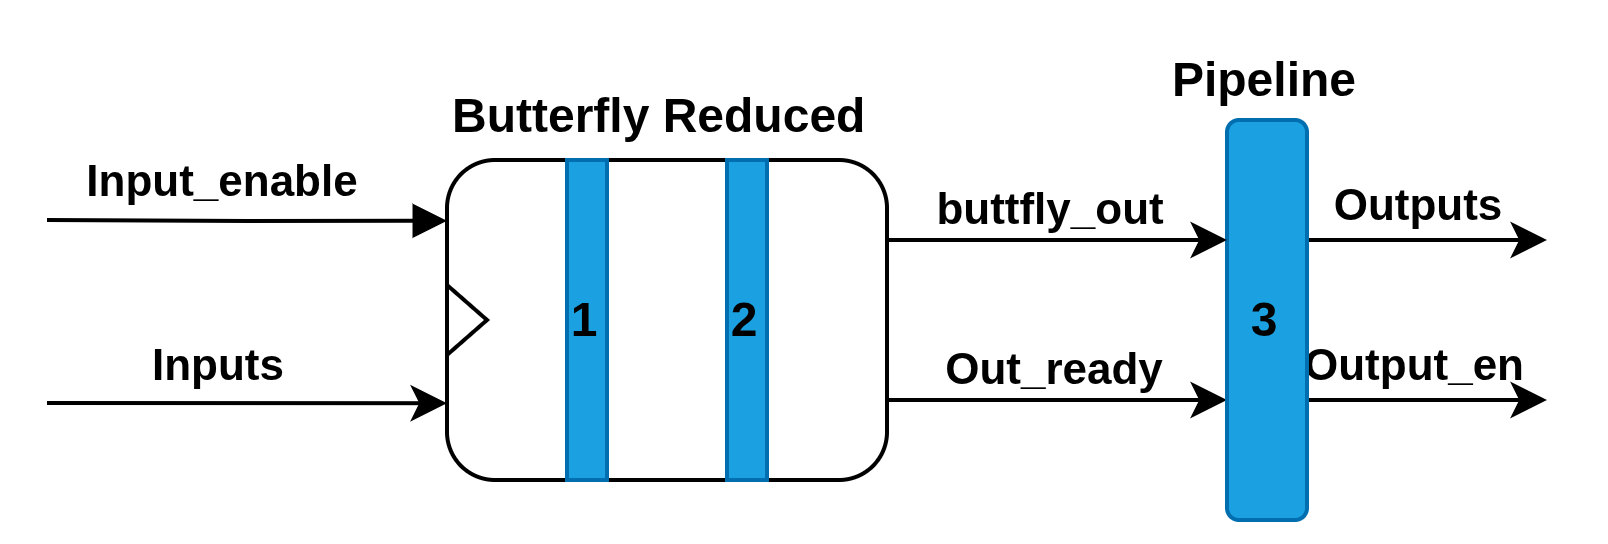
\includegraphics[width=0.8\textwidth]{Images/Stage_1.drawio.png} 
    \caption{Radix-2 fisrt stage top module.}
    \label{fig:Stage_1_r2}
\end{figure}

The first stage is the simplest part of the processor design. Not only is the butterfly unit itself simplified, but the overall stage requires less hardware because no delay registers are needed to align the input data. This can be seen in the far-left stage of the Radix-2 dataflow in Figure \ref{fig:FFT_dataflows}. As a result, the hardware for this first stage consists entirely of just the simplified butterfly unit.

\subsection{Control Unit}
The control unit is responsible for coordinating where inputs are stored, when butterfly operations start, and how the delay buffers function. This is achieved using two counters of variable size, which depends on the stage number.

The first is the \textit{stride segment counter}, which times the writing of new inputs to memory and tracks when the second counter should start. This counter increments every time four new samples arrive (shown as green lines in the graphs).

The second is the \textit{butterfly operation counter}, which starts when the samples required for the butterfly operation arrive. These are the blue samples in the graph, they represent the last samples of a butterfly cluster needed to complete the set of four inputs. Since only one physical butterfly unit exists, we cannot process all four operations at once even if we have the data. Therefore, only one operation happens at a time, and the other data must wait.

To make the design simpler and more portable, these counters do not iterate through all operations in a stage. Instead, each counter counts up to the number of butterflies in the respective cluster (in the graph, this number is 2). The length of these counters is calculated dynamically based on parameters from the SDF unit module that indicate the current stage.

Finally, there are other signals, such as the butterfly counter enable, which validates that the inputs and outputs of the butterfly are valid. There is also a flush counter that tracks the number of remaining operations when the input enable signal goes low. This is needed because the unit requires extra time to finish processing after the last input is received due to the initial delay while waiting for values to arrive.

\begin{figure}[H]
    \centering
    % --- First Row ---
    \begin{subfigure}[b]{0.48\linewidth}
        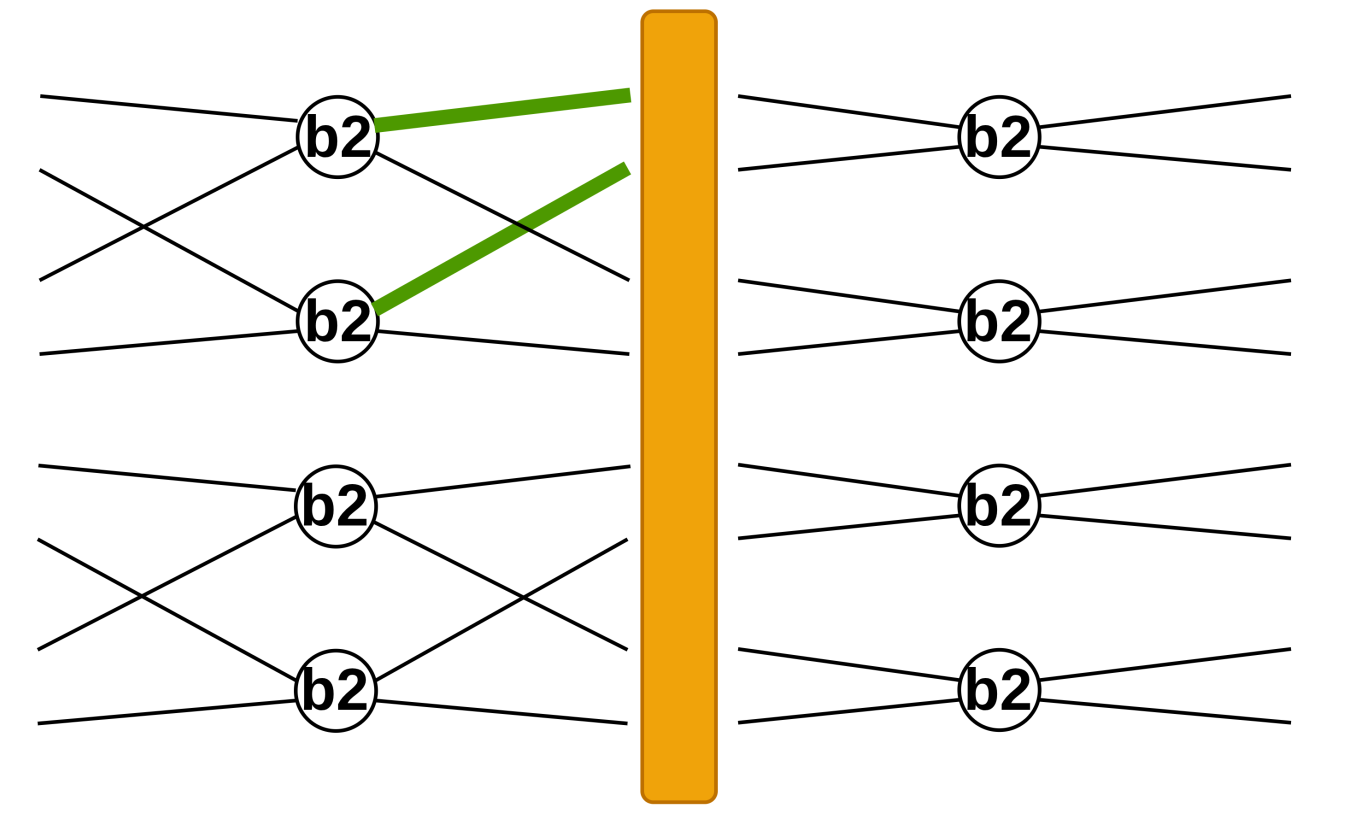
\includegraphics[width=\linewidth]{Images/Control_r2_1.png}
        \caption{Stride counter equals 0}
        \label{fig:tetrada1}
    \end{subfigure}
    \hfill
    \begin{subfigure}[b]{0.48\linewidth}
        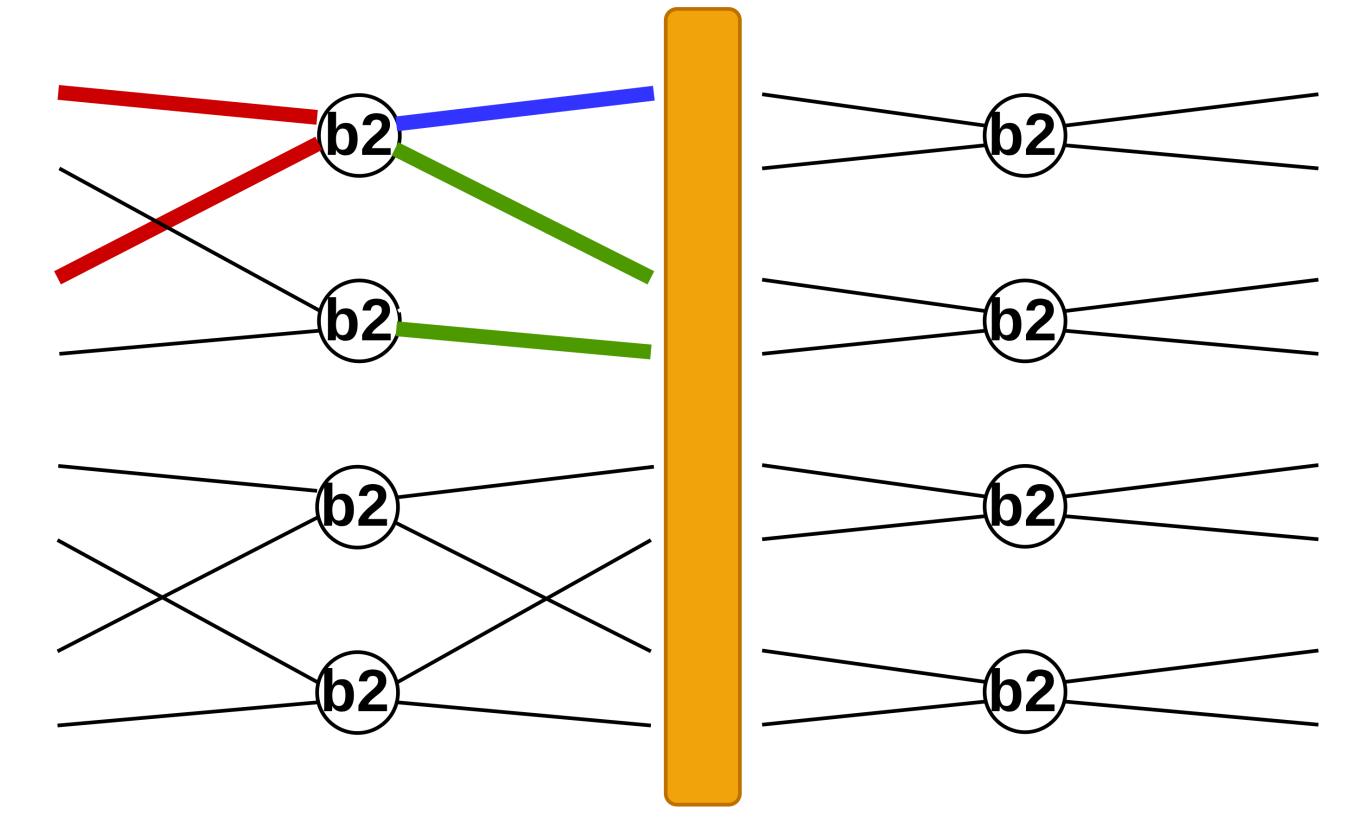
\includegraphics[width=\linewidth]{Images/Control_r2_2.png}
        \caption{Stride counter equals 1 butterfly counter 0}
        \label{fig:tetrada2}
    \end{subfigure}
    
    \vspace{1em}
    
    % --- Second Row ---
    \begin{subfigure}[b]{0.48\linewidth}
        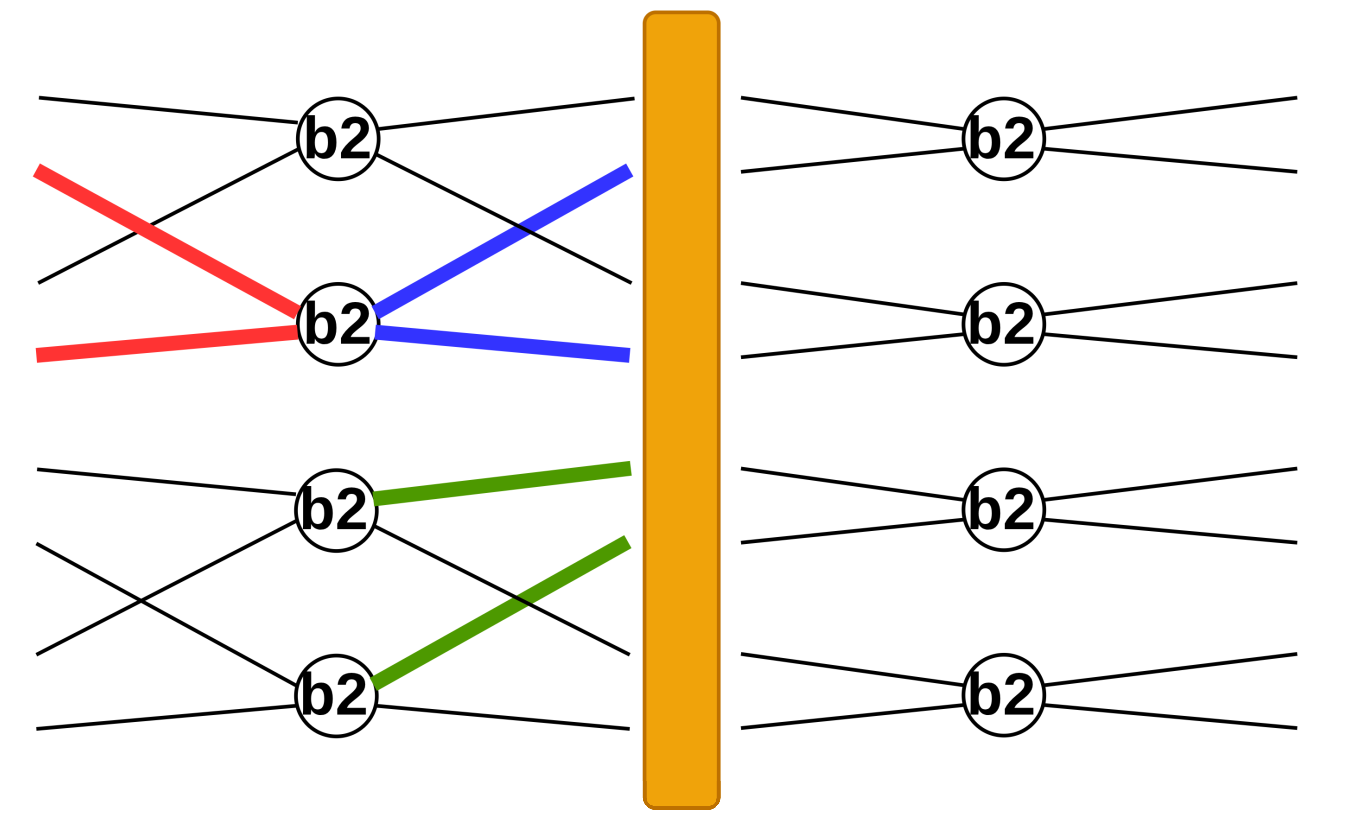
\includegraphics[width=\linewidth]{Images/Control_r2_3.png}
        \caption{Stride counter equals 0, butterfly counter 1}
        \label{fig:tetrada3}
    \end{subfigure}
    \hfill
    \begin{subfigure}[b]{0.48\linewidth}
        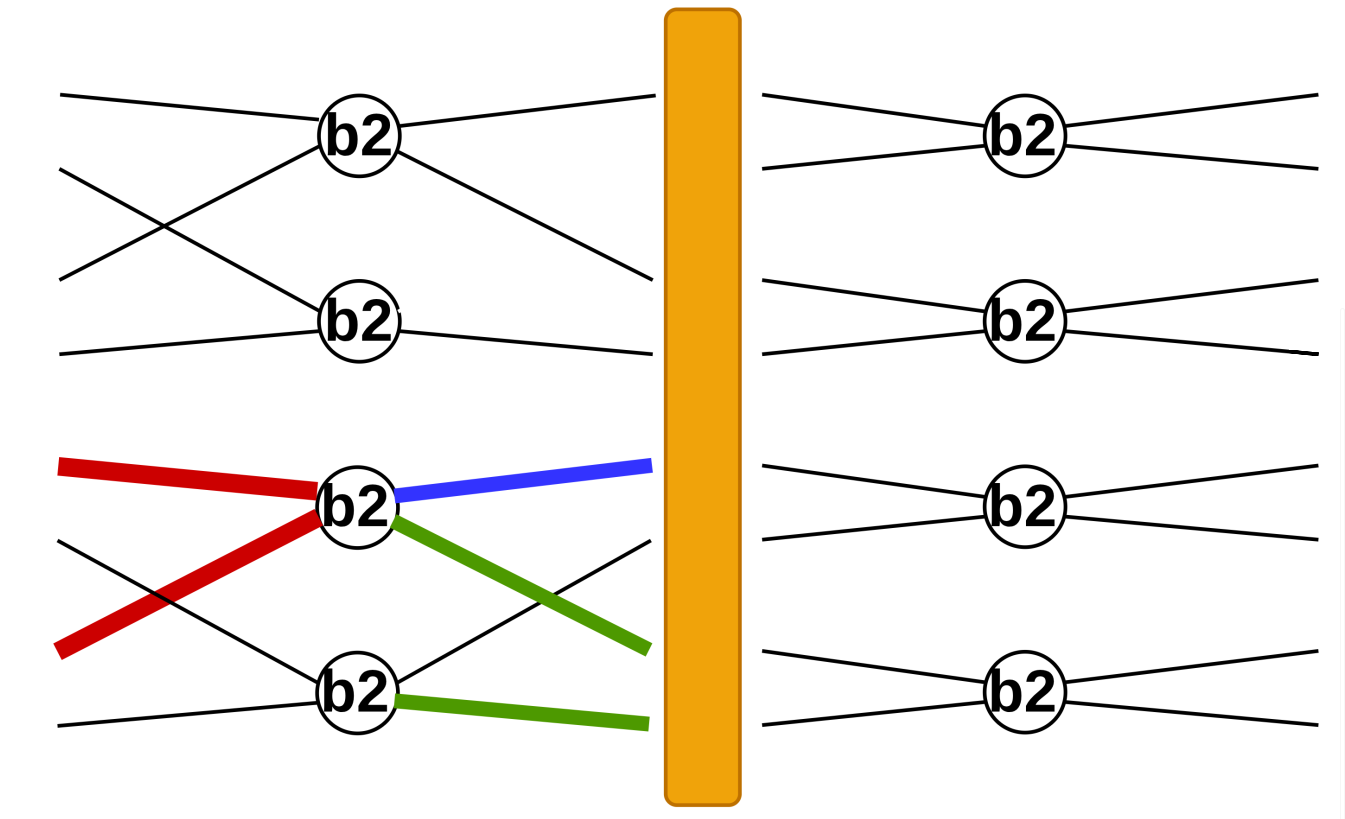
\includegraphics[width=\linewidth]{Images/Control_r2_4.png}
        \caption{Stride counter equals 1, butterfly counter 0}
        \label{fig:tetrada4}
    \end{subfigure}
    
    \caption{Operation flow of the counters managing the pairs of data points.}
    \label{fig:all_tetradas}
\end{figure}

\subsection{Delay Registers and Final Design}
To properly align the incoming data, it must be stored temporarily. We achieve this by using simple delay buffers with an adjustable (parameterizable) depth. This allows the same buffer design to be reused across all stages, even though each stage requires a different latency.

For this design, only two delay registers are needed per stage. Their depths are calculated as:
\begin{itemize}
    \item $\mathrm{Depth\_A} = 2^{\mathrm{STAGE\_NUM} - 1}$ 
    \item $\mathrm{Depth\_B} = \mathrm{Depth\_A} \times 2$
\end{itemize}

Because the buffer depth doubles with each additional stage, the overall hardware area increases exponentially for larger FFT sizes. With the addition of these delay registers, the Stage module is complete. In the diagram, the output dataflow pipelines are highlighted in blue, and the input dataflow pipelines are highlighted in green.

\begin{figure}[H]
    \centering
    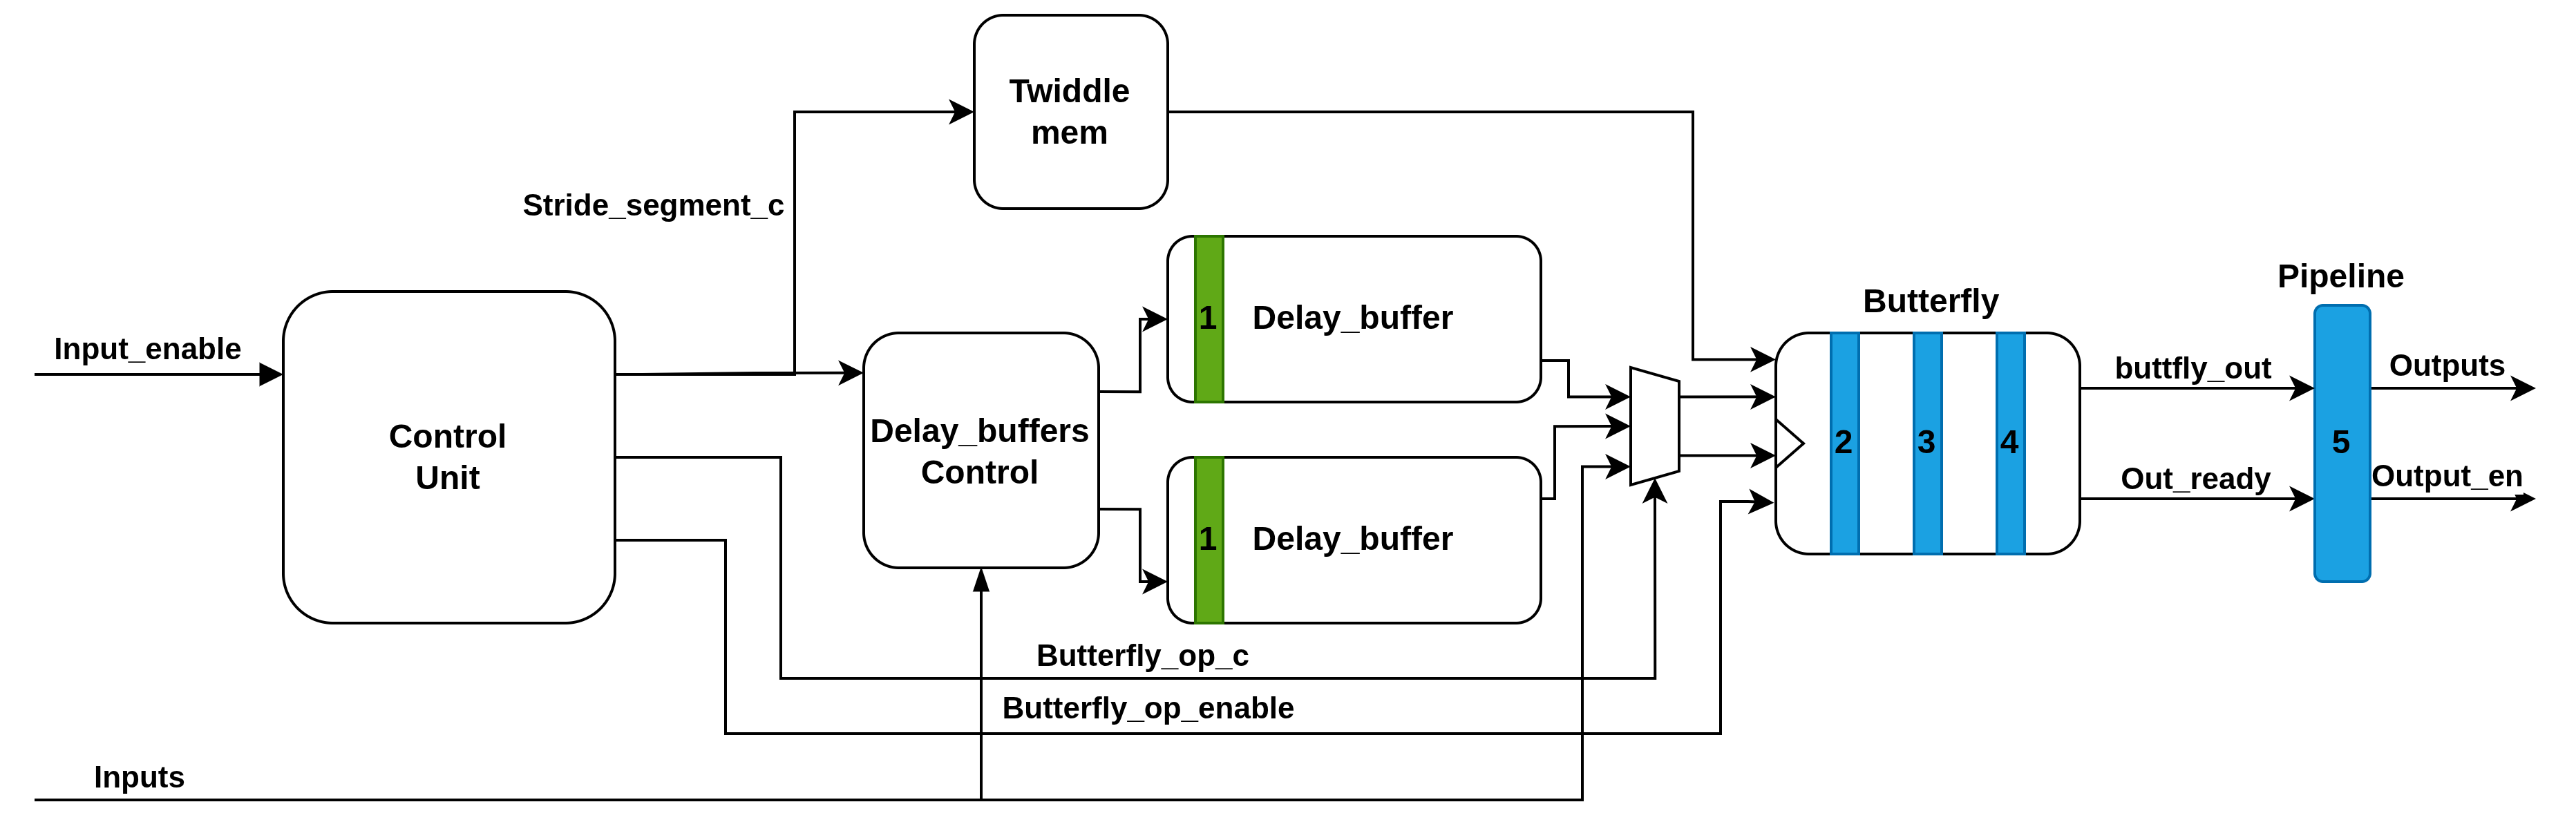
\includegraphics[width=1\textwidth]{Images/Radix-2_stage_unit.drawio.png} 
    \caption{Radix-2 general stage unit top module.}
    \label{fig:Stage_1_r2}
\end{figure}

In the top-level module, which connects all stage units to form a complete FFT, each stage's outputs are chained directly to the next stage's inputs. The first stage receives the input samples, and the final stage produces the results.

To accommodate bit growth, each stage instantiation can have a different data width. The top module calculates the maximum required bit width based on the input parameters, and the RTL dynamically scales the bit width for the specific stages that require it. For example, if the starting parameters specify a data width of 14 and a twiddle width of 10, the top module will only begin increasing the bit size after the fourth stage.

Because unoptimized widths can waste resources, the general rule for this design is that the starting data width should be equal to the twiddle width plus one. This constraint is not enforced automatically in the RTL solely to provide greater flexibility for testing and simulating the design.

\subsection{Implementation Results using an ISO Clock}
These implementations utilize a generous clock frequency of 100 MHz (a 10 ns clock period) and an 8-bit twiddle factor width to highlight the area differences between the implemented algorithms on an Artix-7 AC701 Evaluation Platform (\texttt{xc7a200tfbg676-2}). Furthermore, only powers-of-four FFT sizes are presented to ensure direct comparability with subsequent radix-4 designs.

\begin{figure}[H]
    \centering
    \begin{tikzpicture}
        \begin{axis}[
            ybar,
            width=0.9\textwidth,
            height=7.5cm,
            ylabel={Resource Count},
            symbolic x coords={256-Trad, 256-Gauss, 1024-Trad, 1024-Gauss, 4096-Trad, 4096-Gauss},
            xtick=data,
            x tick label style={rotate=30, anchor=east, font=\scriptsize},
            nodes near coords,
            every node near coord/.append style={font=\tiny, rotate=90, anchor=west},
            legend style={at={(0.5,-0.25)}, anchor=north, legend columns=-1},
            title={Resource Utilization Across FFT Sizes and Multiplier Types},
            ymin=0,
            enlarge x limits=0.15,
            bar width=6pt,
        ]
            % LUTs
            \addplot coordinates {
                (256-Trad, 1453) (256-Gauss, 1641) 
                (1024-Trad, 3060) (1024-Gauss, 3287) 
                (4096-Trad, 8837) (4096-Gauss, 9121)
            };
            
            % Registers
            \addplot coordinates {
                (256-Trad, 1713) (256-Gauss, 1714) 
                (1024-Trad, 2335) (1024-Gauss, 2360) 
                (4096-Trad, 3100) (4096-Gauss, 3060)
            };
            
            % DSPs
            \addplot coordinates {
                (256-Trad, 28) (256-Gauss, 21) 
                (1024-Trad, 36) (1024-Gauss, 27) 
                (4096-Trad, 44) (4096-Gauss, 33)
            };
            
            \legend{LUTs, Registers, DSPs}
        \end{axis}
    \end{tikzpicture}
    \caption{Utilization comparison (LUTs, Registers, and DSPs) for Radix-2 FFT implementations across sizes 256, 1024, and 4096 under ISO clock constraints.}
    \label{fig:radix2_all_resources_combined}
\end{figure}

\begin{table}[H]
    \centering
    \caption{FIFO Radix-2 Latency.}
    \vspace{0.5em}
    \begin{tabular}{lcccc}
        \hline
        \textbf{Metric} & \textbf{New-256} & \textbf{New-1024} & \textbf{New-4096} & \textbf{New-256} \\
        \hline
        Latency Trad (cycles) & 165 & 559 & 2105 & 259 \\
        Latency Gauss (cycles) & 172 & 568 & 2116 & -- \\
        \hline
    \end{tabular}
    \label{tab:baseline_results_256}
\end{table}

Due to the registers used for data alignment, the register growth for 4096 samples is substantial, and a closer inspection reveals that it doubles with each successive increase in FFT size. Furthermore, a comparison between the legacy 256-point and new 256-point FFT implementations shows a reduction in overall latency. Although the throughput is doubled, the latency is not reduced by half; this is caused by the extra pipelining introduced in the new stage unit, which adds a constant cycle penalty but ultimately yields significantly better timing results.

\section{Radix-4 Implementation}

\subsection{Overview of Proposed Implementation}
For the implementation of the Radix-4 algorithm, a methodology similar to that of the Radix-2 design is adopted. The architecture is configured to achieve the maximum throughput supported by the Radix-4 butterfly (four samples per clock cycle), while exploring alternative buffering strategies to efficiently store and align the data. As with the preceding design, this implementation follows a Decimation-in-Time (DIT) structure, requiring the input sequence to be supplied in digit-reversed order (base-4 reversal).

\subsection{Butterfly Radix-4}
Algorithm \ref{alg:radix4_butterfly} operates similarly to the Radix-2 butterfly, but is adapted for Radix-4 arithmetic. It reuses the same multiplication techniques and requires delay registers to align the $A$ inputs with the outputs of the multipliers.

Analyzing the arithmetic operations within the butterfly module, it is evident that the required bit growth between stages is 2 bits, due to the two consecutive additions performed at the end of the butterfly.

\begin{algorithm}
\caption{Pipelined Radix-4 Butterfly}
\label{alg:radix4_butterfly}
\begin{algorithmic}[1]
\Require Complex inputs $A$, $B$, $C$, $D$; twiddle factors $W_0$, $W_1$, $W_2$; $start$ signal
\Ensure  Complex outputs $Out_1$, $Out_2$, $Out_3$, $Out_4$; $done$ signal

\Statex \textbf{Step 1: Complex multiplication of $B$, $C$, $D$ by $W_0$, $W_1$, $W_2$}
\If{$\mathit{stage\_num} = 1$}
    \State $B_{\mathit{mult}} \gets B \ll (\mathit{Tw\_Width} - 1)$ \Comment{Shift replaces multiplier}
    \State $C_{\mathit{mult}} \gets C \ll (\mathit{Tw\_Width} - 1)$ 
     $D_{\mathit{mult}} \gets D \ll (\mathit{Tw\_Width} - 1)$ 
\ElsIf{$\mathit{SimpleMult} = 1$}
    \State $B_{\mathit{mult}} \gets \Call{SimpleMult}{B, W_0}$ \Comment{Traditional complex multiplier}
    \State $C_{\mathit{mult}} \gets \Call{SimpleMult}{C, W_1}$ 
     $D_{\mathit{mult}} \gets \Call{SimpleMult}{D, W_2}$ 
\Else
    \State $B_{\mathit{mult}} \gets \Call{CheapMult}{B, W_0}$ \Comment{Gauss complex multiplier}
    \State $C_{\mathit{mult}} \gets \Call{CheapMult}{C, W_1}$
     $D_{\mathit{mult}} \gets \Call{CheapMult}{D, W_2}$ 
\EndIf

\Statex \textbf{Step 2: Pipeline balancing}
\State $A_{\mathit{delayed}} \gets \Call{Delay}{A, \mathit{delay\_mult} + 1}$ \Comment{Match multiplier latency + scale reg}
\State $done \gets \Call{Delay}{start, \mathit{delay\_mult} + 3}$ \Comment{Match total pipeline latency}

\Statex \textbf{Step 3: Scaling}
\State $B_{\mathit{scaled}} \gets \Call{Truncate}{B_{\mathit{mult}}, \mathit{Tw\_Width} - 1}$ \Comment{Remove twiddle scaling}
\State $C_{\mathit{scaled}} \gets \Call{Truncate}{C_{\mathit{mult}}, \mathit{Tw\_Width} - 1}$ 
\State $D_{\mathit{scaled}} \gets \Call{Truncate}{D_{\mathit{mult}}, \mathit{Tw\_Width} - 1}$ 

\Statex \textbf{Step 4: Butterfly Stage 1 (Intermediate variables)}
\State $t_0 \gets A_{\mathit{delayed}} + C_{\mathit{scaled}}$
\State $t_1 \gets A_{\mathit{delayed}} - C_{\mathit{scaled}}$
\State $t_2 \gets B_{\mathit{scaled}} + D_{\mathit{scaled}}$
\State $t_3 \gets B_{\mathit{scaled}} - D_{\mathit{scaled}}$

\Statex \textbf{Step 5: Butterfly Stage 2 (Outputs)}
\State $Out_1 \gets t_0 + t_2$
\State $Out_2 \gets t_1 - j \cdot t_3$ \Comment{Implemented as $t_{1r} + t_{3i}$ and $t_{1i} - t_{3r}$}
\State $Out_3 \gets t_0 - t_2$
\State $Out_4 \gets t_1 + j \cdot t_3$ \Comment{Implemented as $t_{1r} - t_{3i}$ and $t_{1i} + t_{3r}$}
\end{algorithmic}
\end{algorithm}

\subsection{First Stage}
\begin{figure}[H]
    \centering
    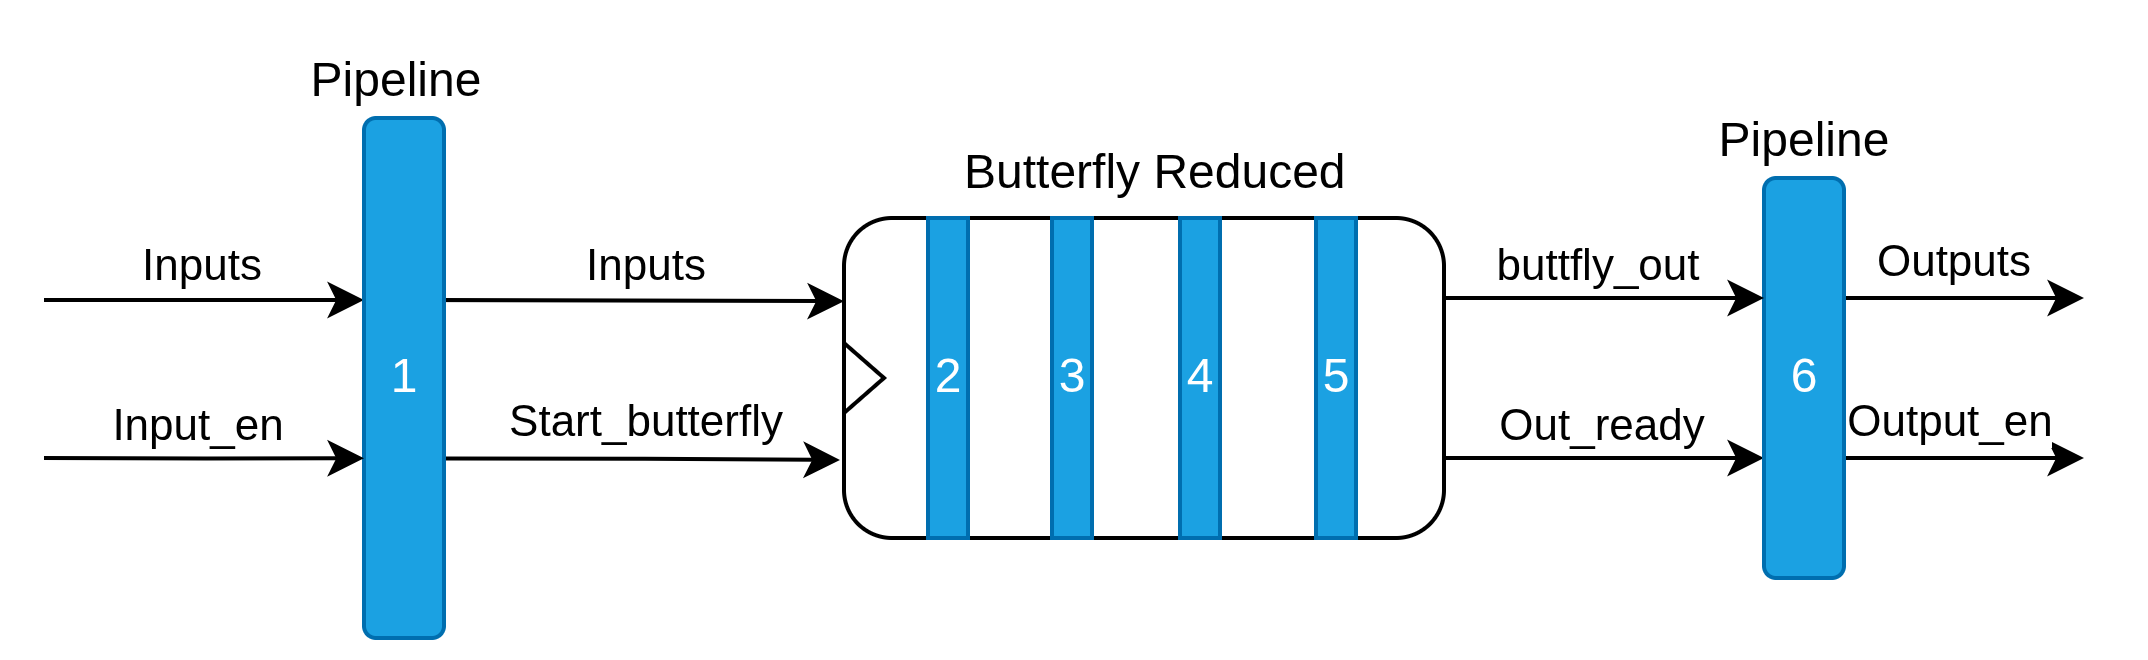
\includegraphics[width=0.8\textwidth]{Images/Stage_1_r4.drawio.png} 
    \caption{Radix-4 fisrt stage top module.}
    \label{fig:Stage_1_r2}
\end{figure}

The first stage is again the simplest part of the processor design.  The butterfly unit itself is simplified and the overall stage requires less hardware because no delay registers are needed to align the input data. This can be seen in the far-left stage of the Radix-4 dataflow in Figure \ref{fig:FFT_dataflows}. As a result, the hardware for this first stage consists entirely of just the simplified butterfly unit.

\subsection{Control Unit}
\begin{figure}[H]
    \centering
    % --- First Row ---
    \begin{subfigure}[b]{0.3\linewidth}
        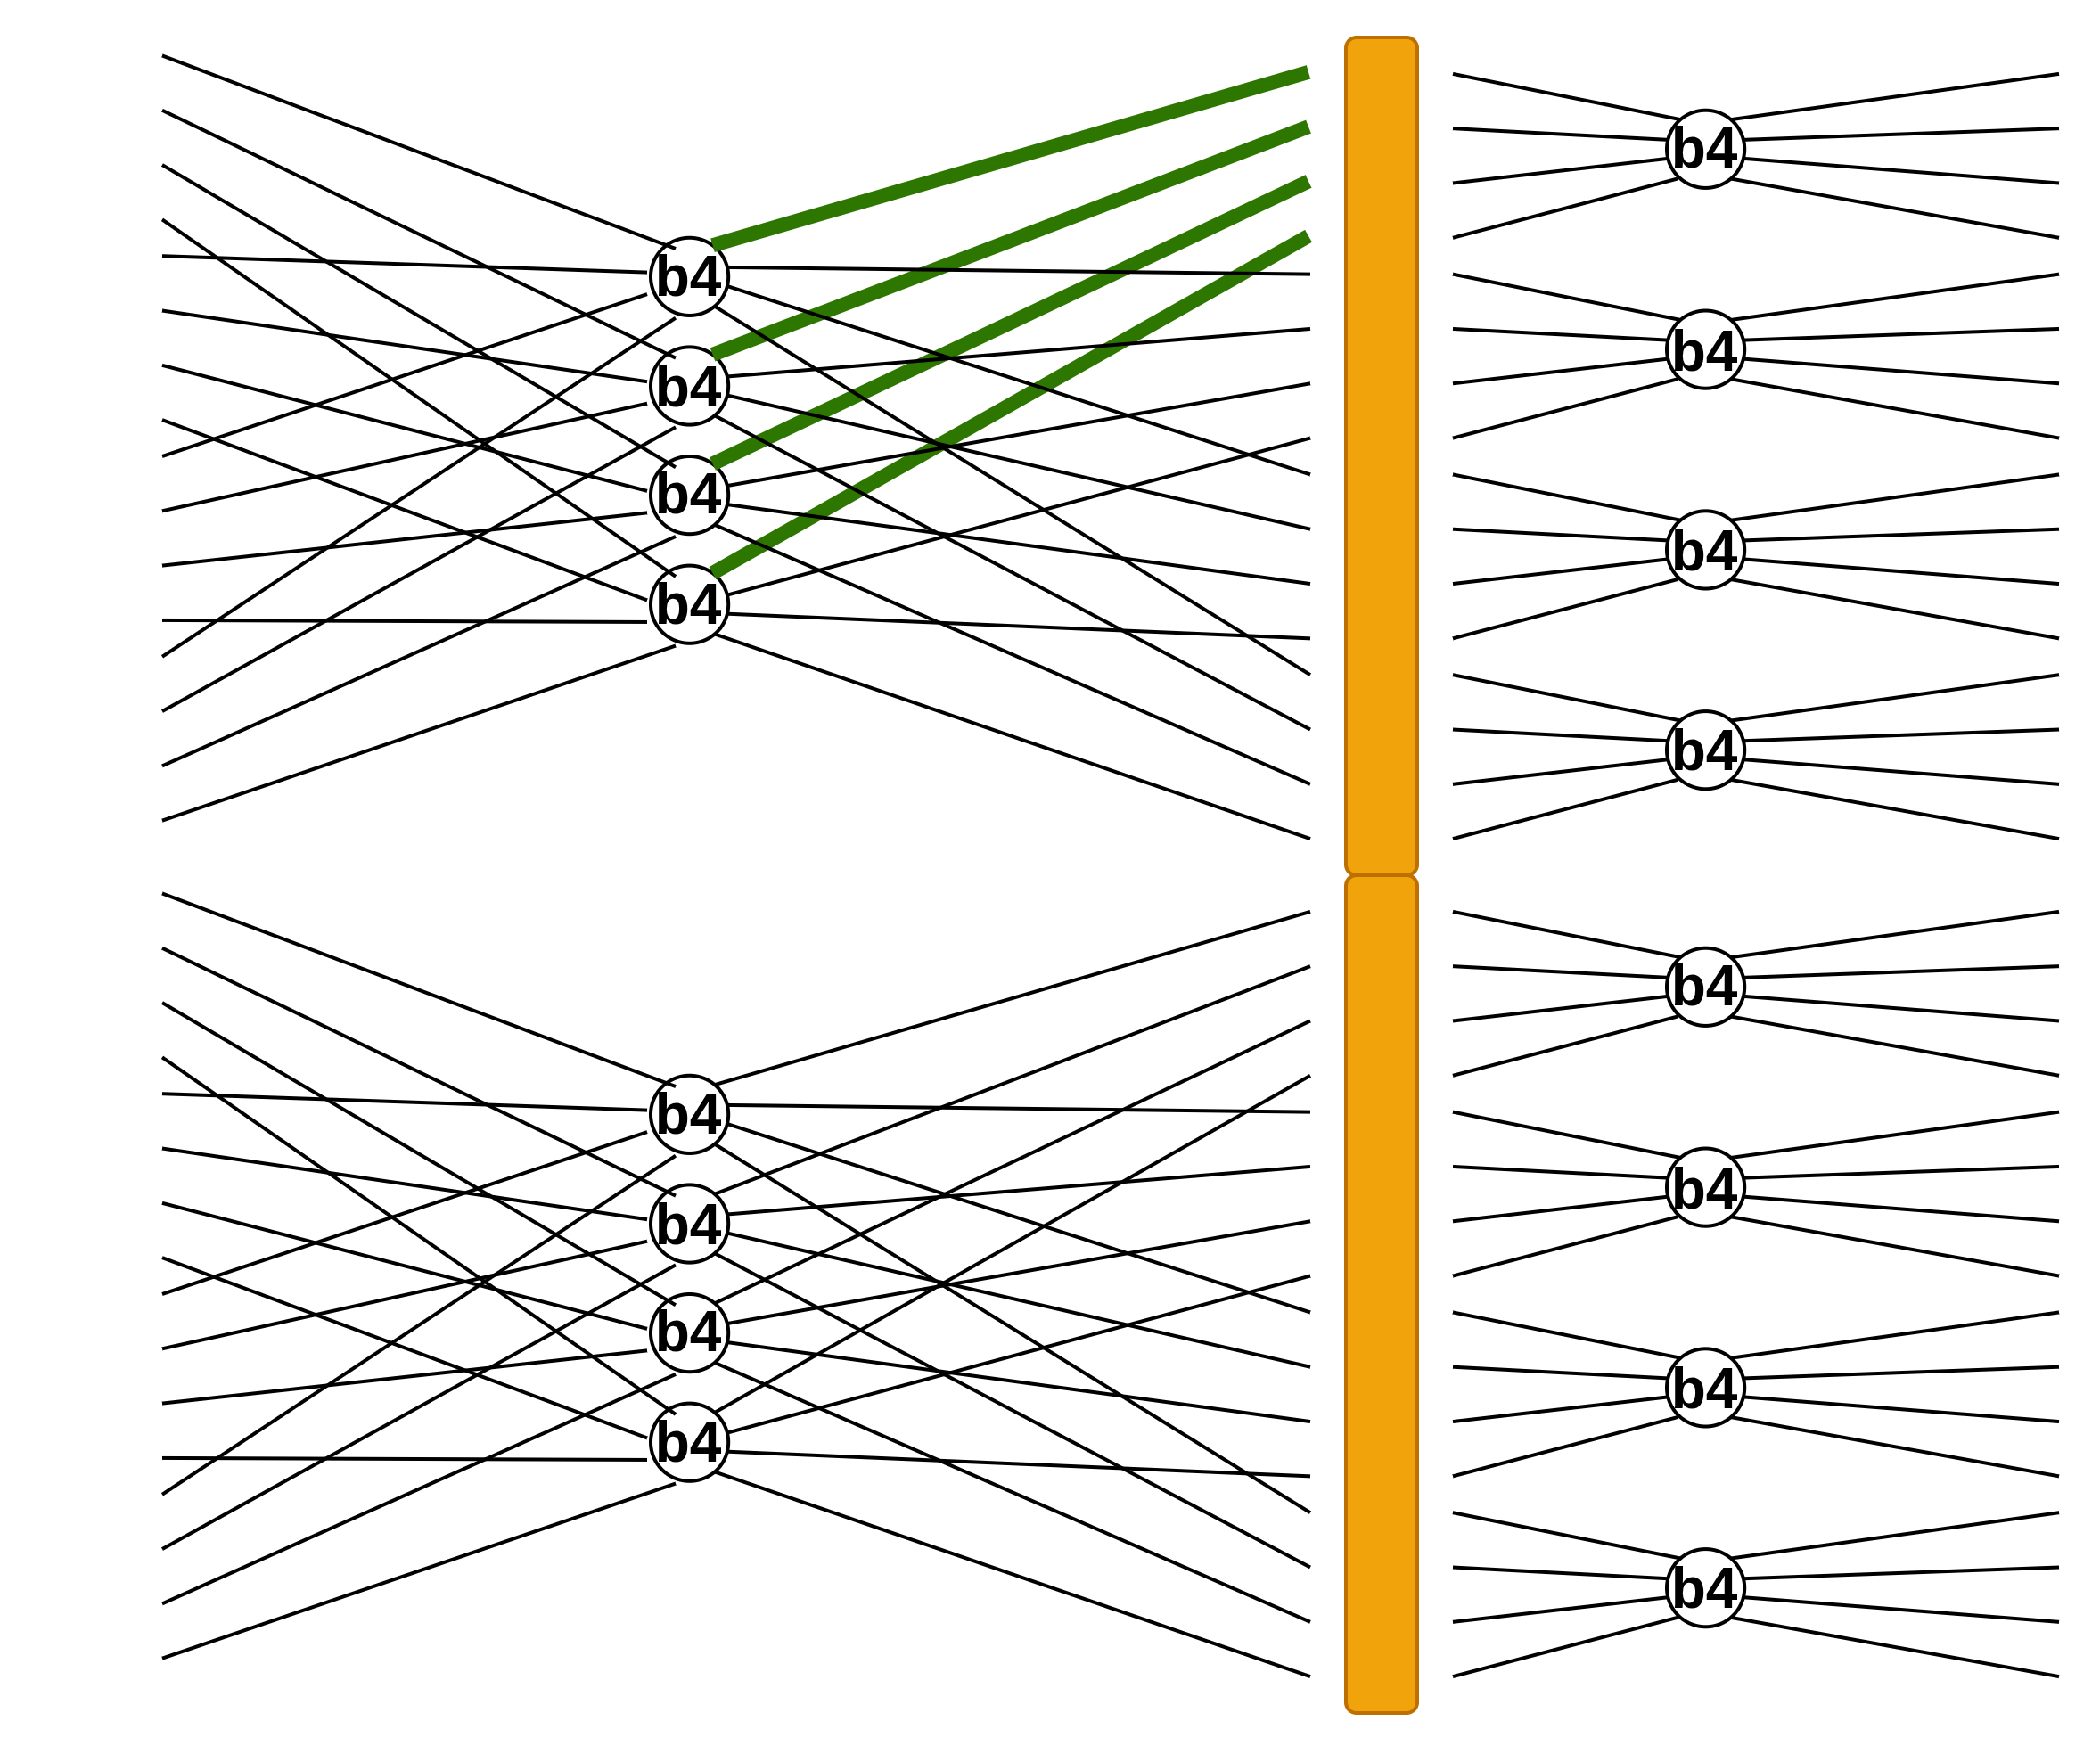
\includegraphics[width=\linewidth]{Images/1st_tetrada.png}
        \caption{Stride counter equals 00}
        \label{fig:tetrada1}
    \end{subfigure}
    \hfill
    \begin{subfigure}[b]{0.3\linewidth}
        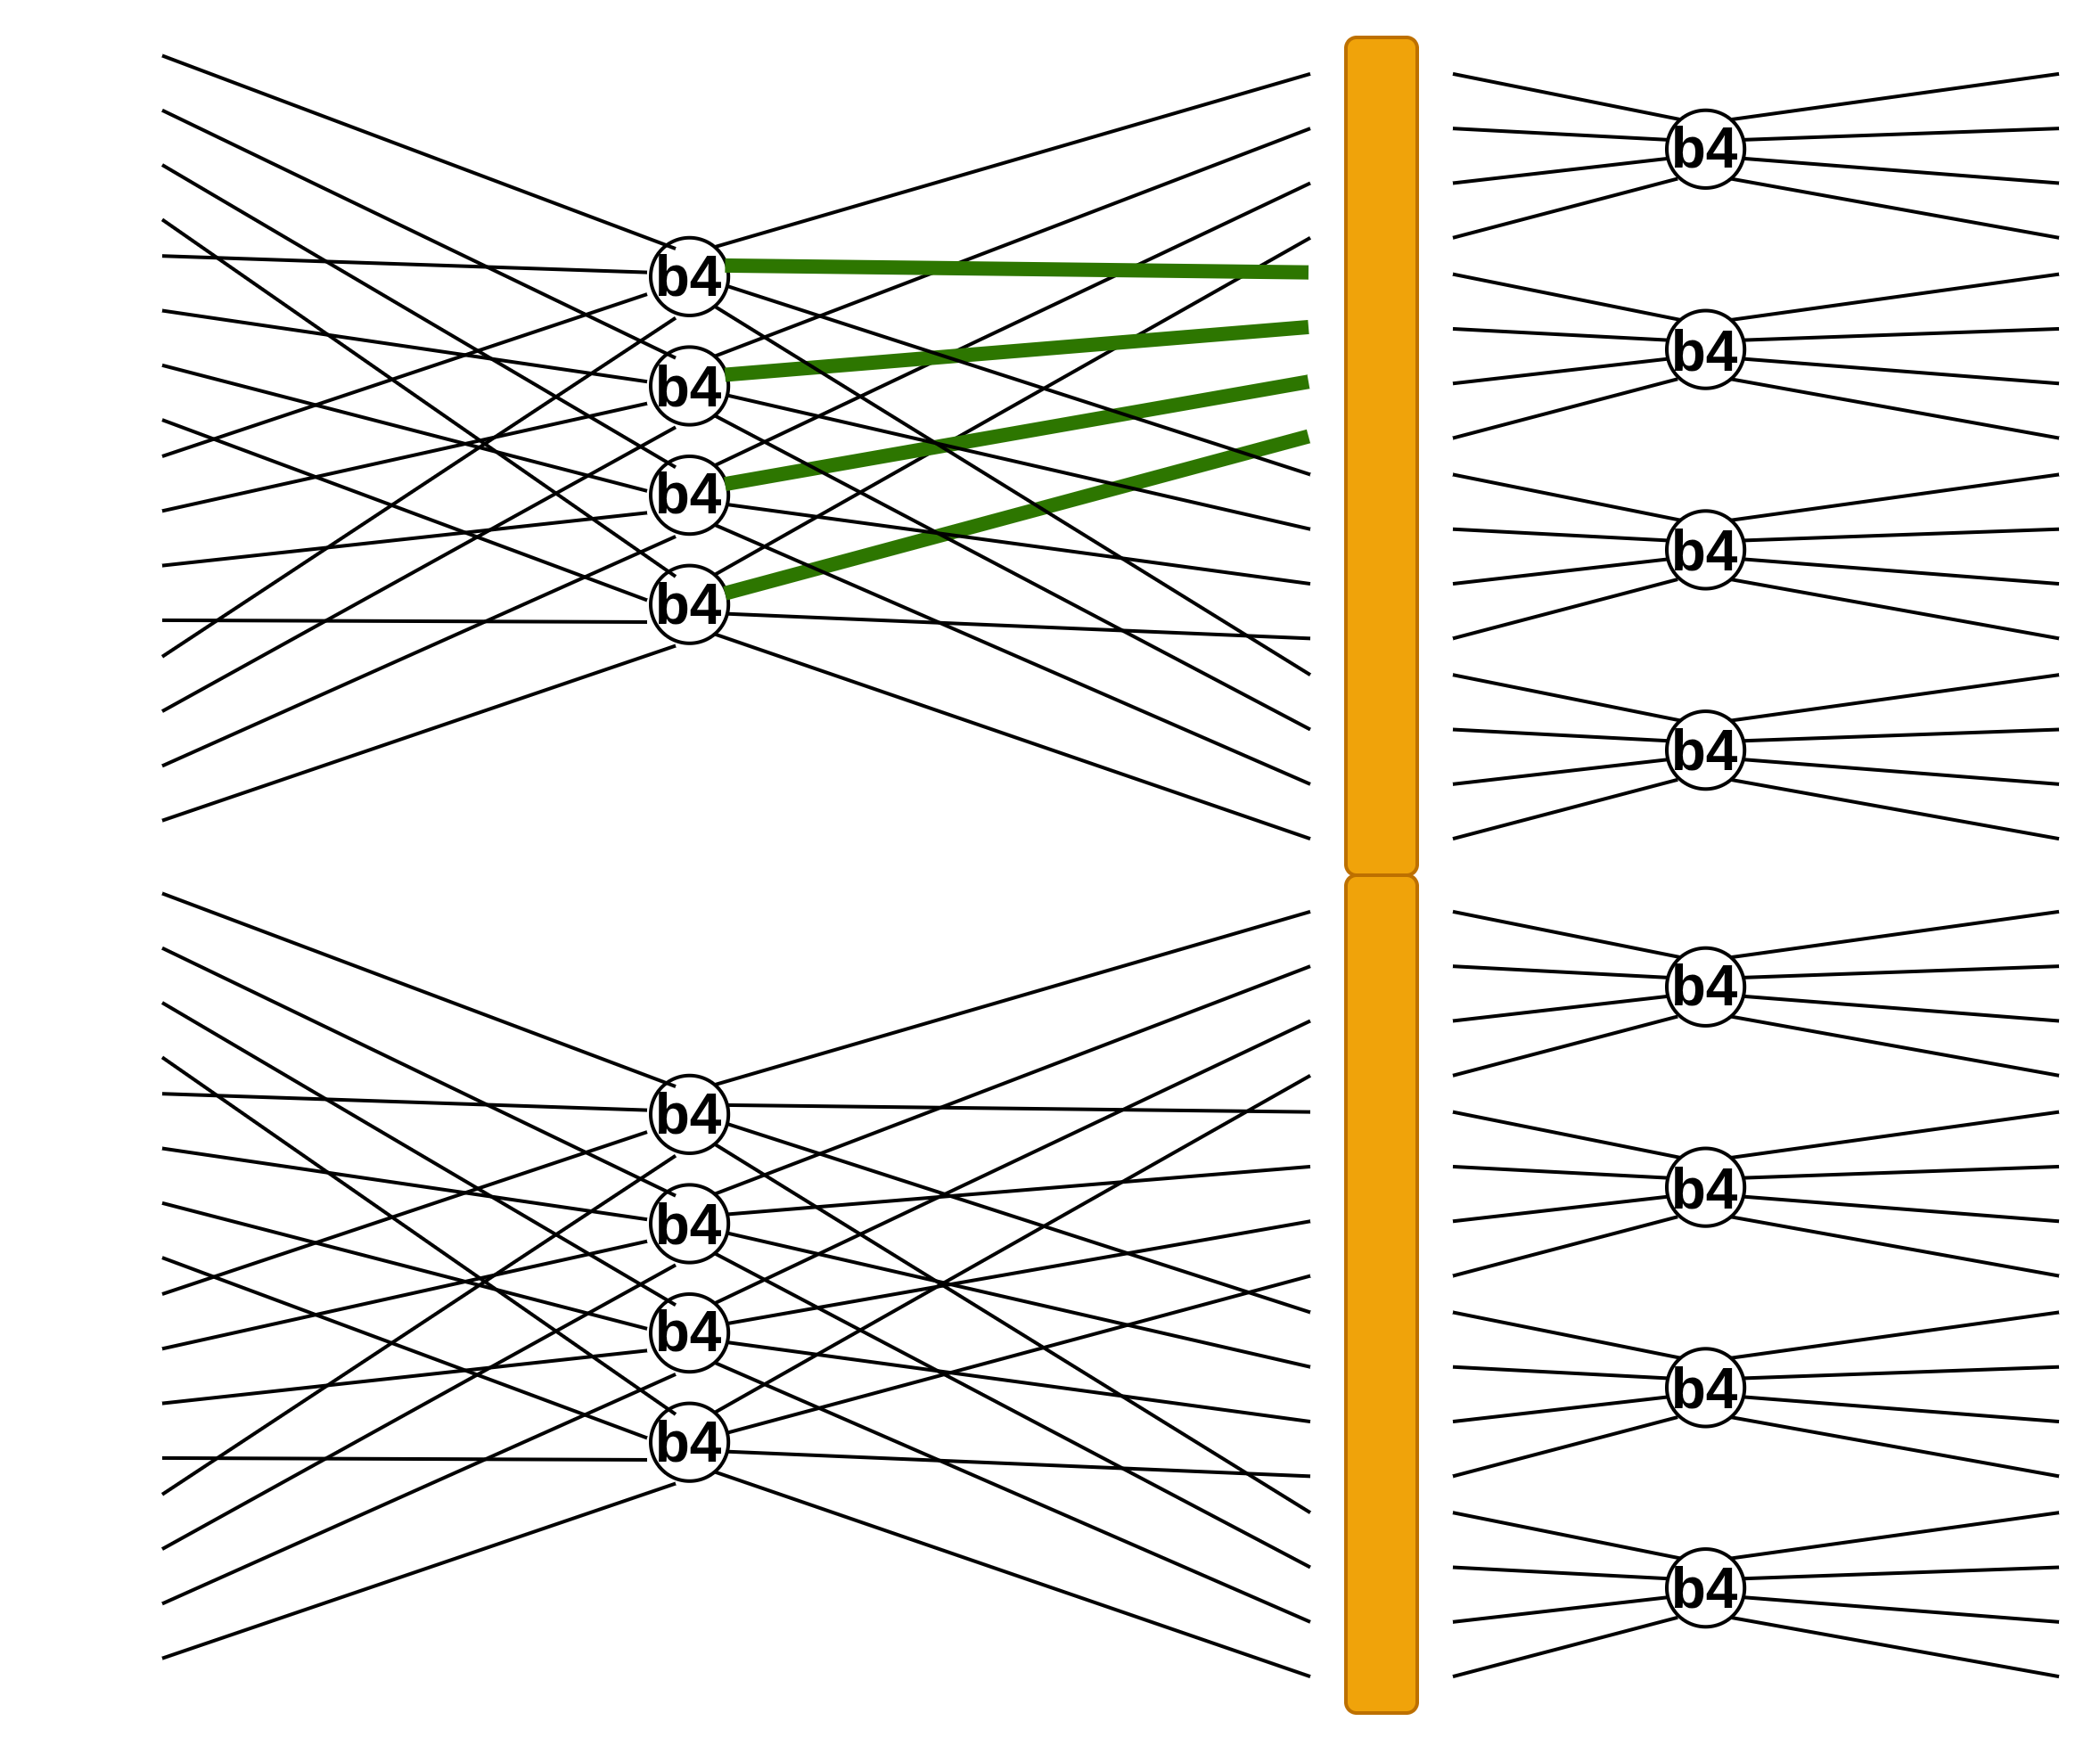
\includegraphics[width=\linewidth]{Images/2nd_tetrada.png}
        \caption{Stride counter equals 01}
        \label{fig:tetrada2}
    \end{subfigure}
    \hfill
    \begin{subfigure}[b]{0.3\linewidth}
        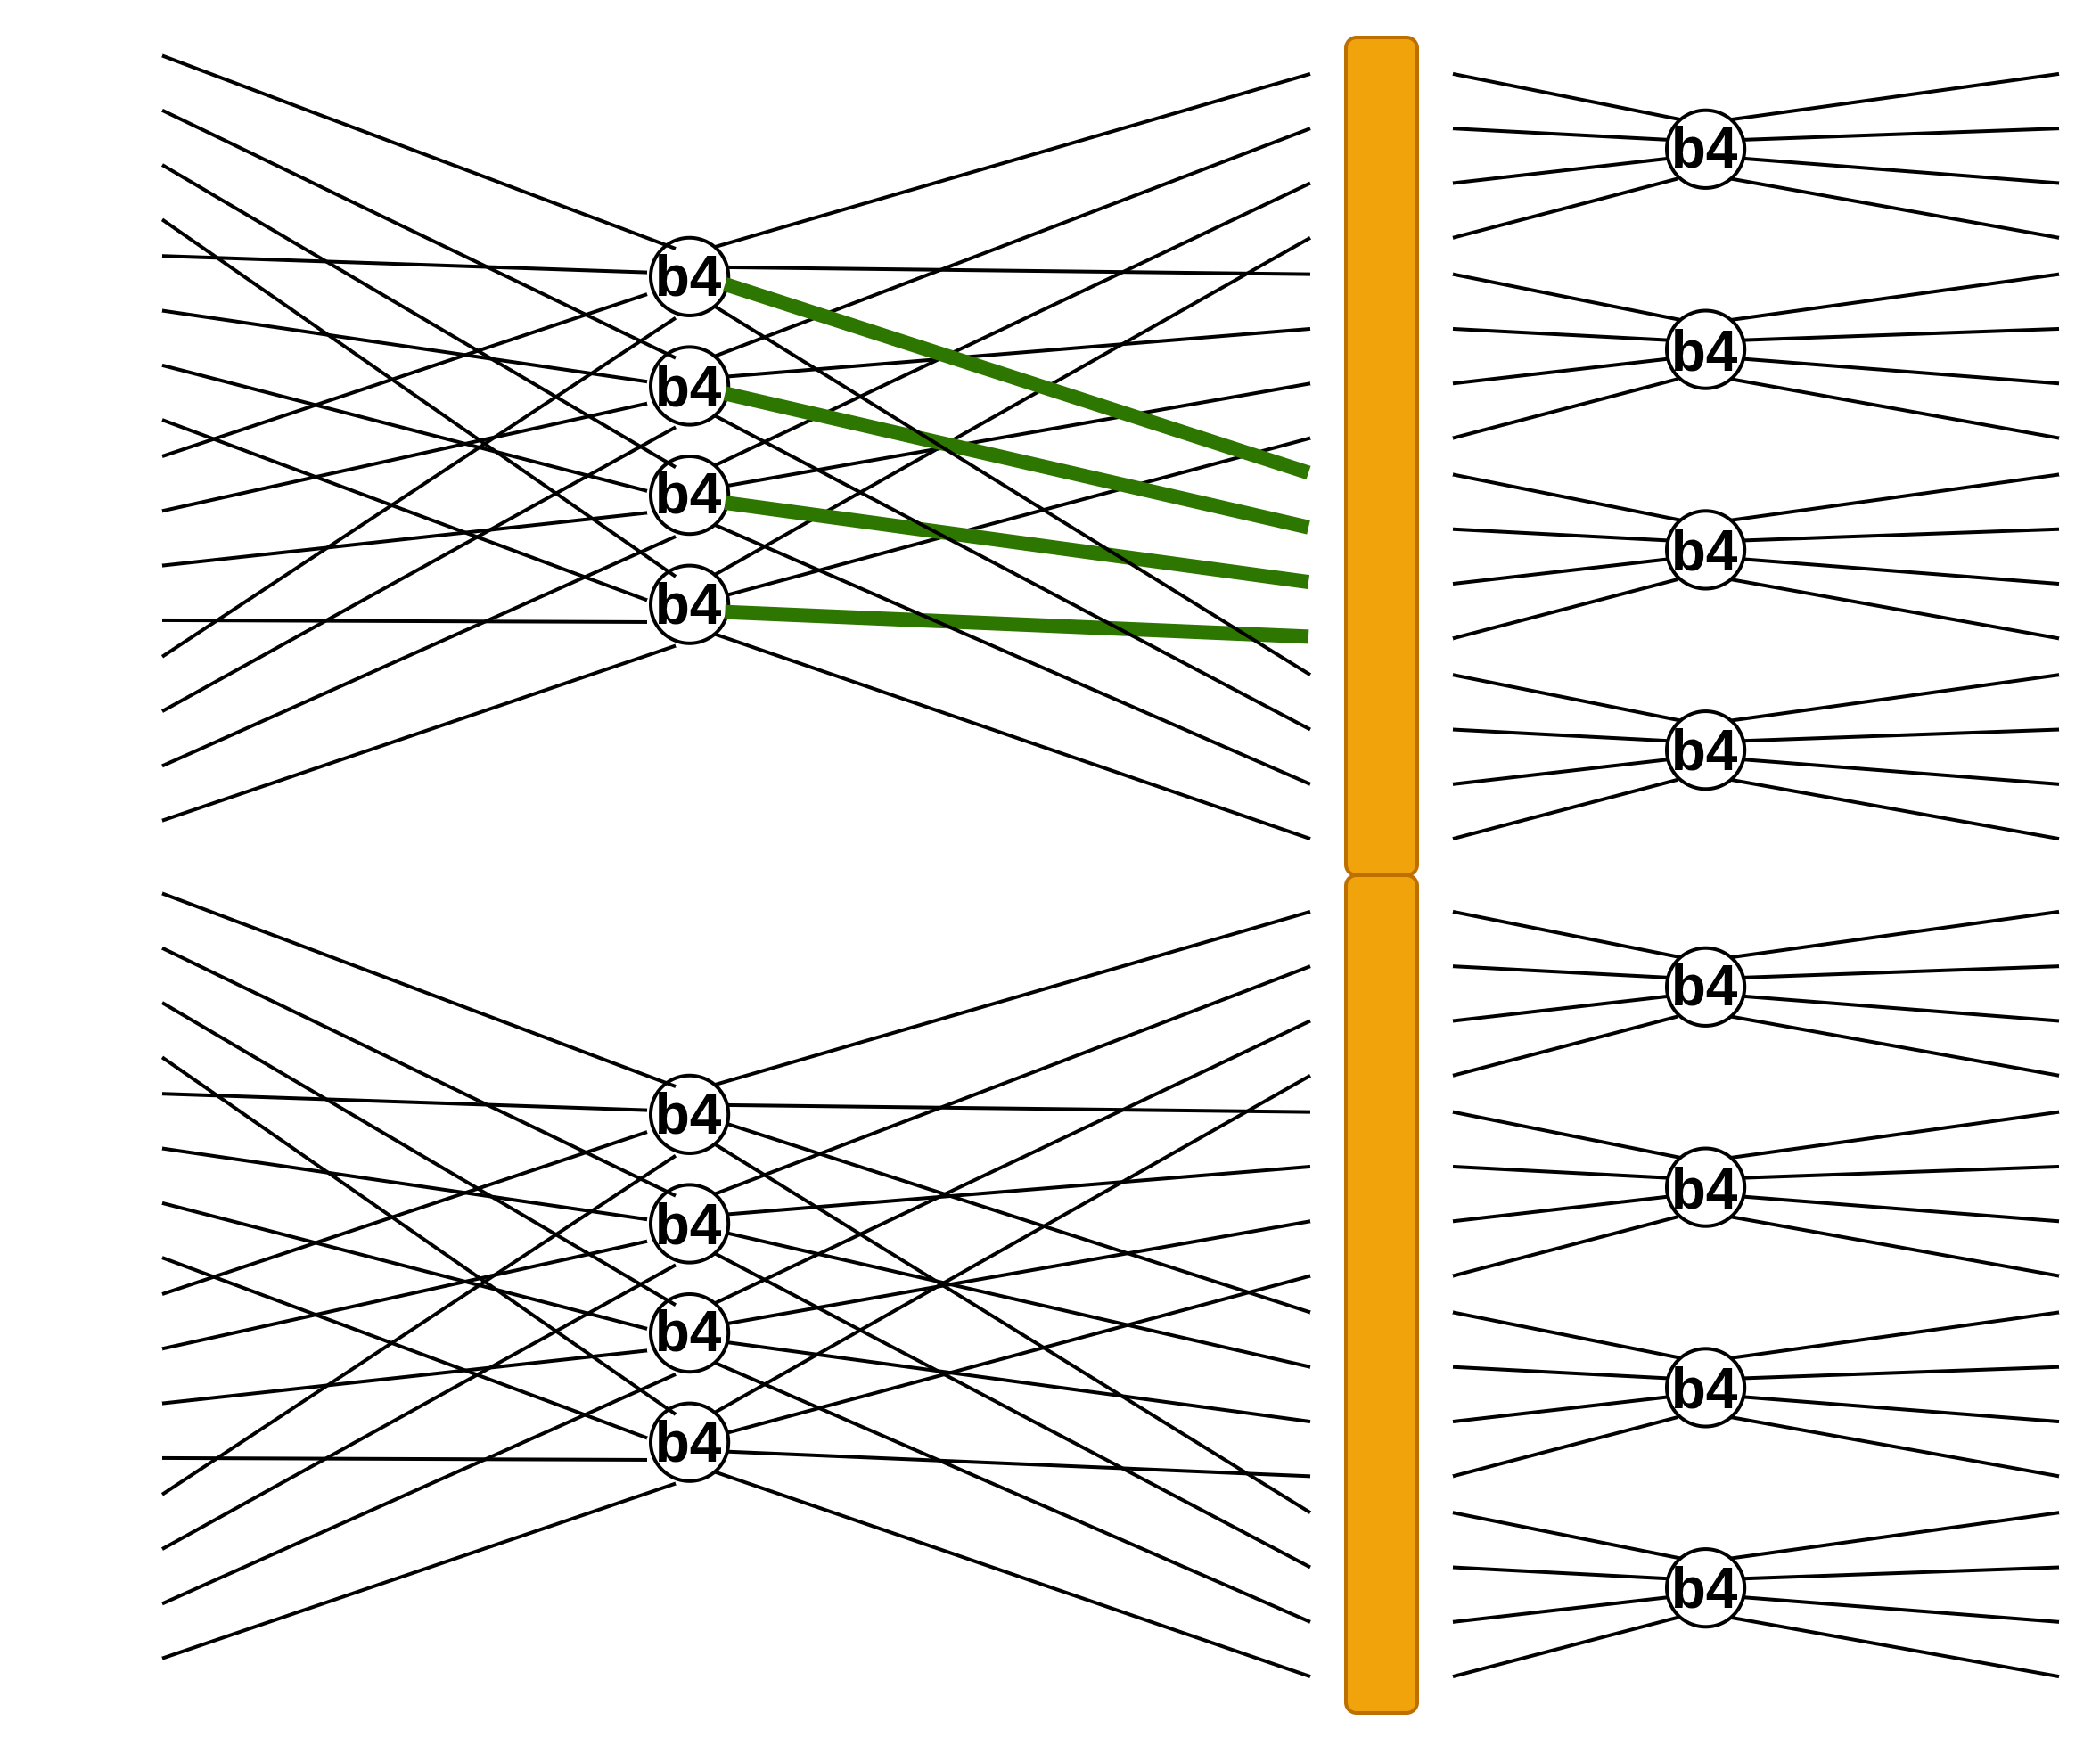
\includegraphics[width=\linewidth]{Images/3rd_tetrada.png}
        \caption{Stride counter equals 10, butterfly counter starts}
        \label{fig:tetrada3}
    \end{subfigure}
    
    \vspace{1em}
    
    % --- Second Row ---
    \begin{subfigure}[b]{0.3\linewidth}
        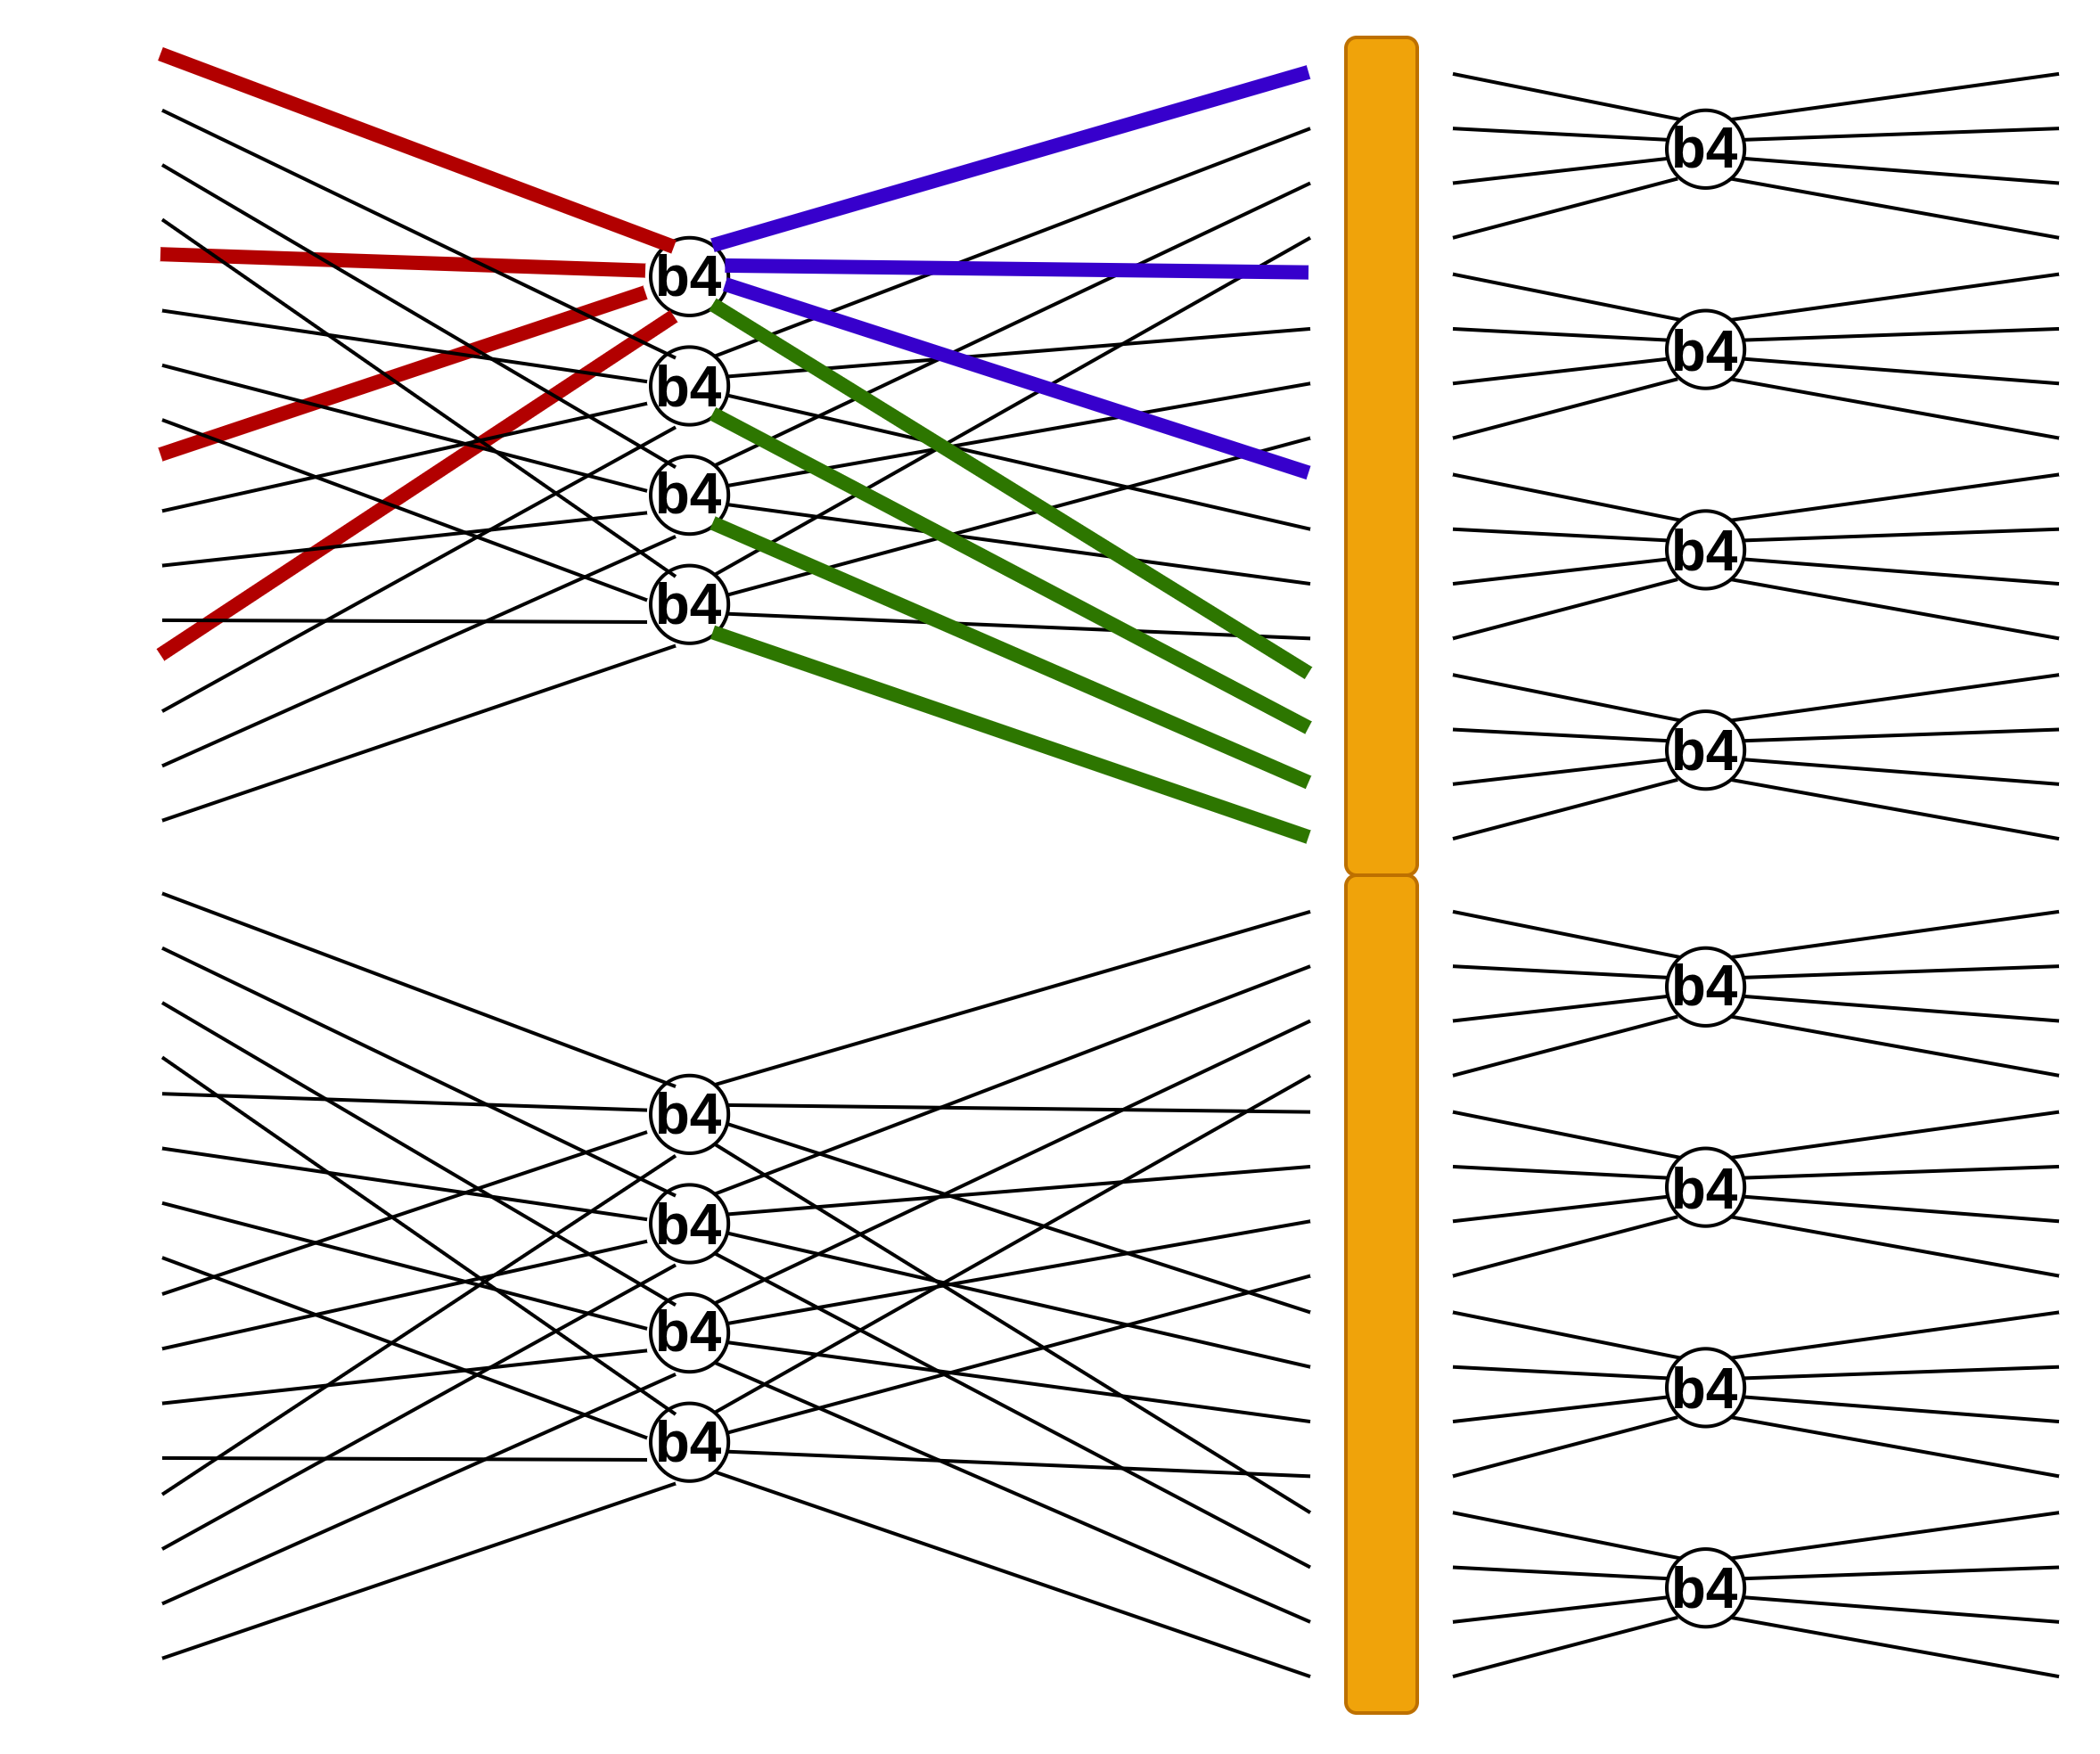
\includegraphics[width=\linewidth]{Images/4th_tetrada.png}
        \caption{Stride counter equals 11, butterfly counter 00}
        \label{fig:tetrada4}
    \end{subfigure}
    \hfill
    \begin{subfigure}[b]{0.3\linewidth}
        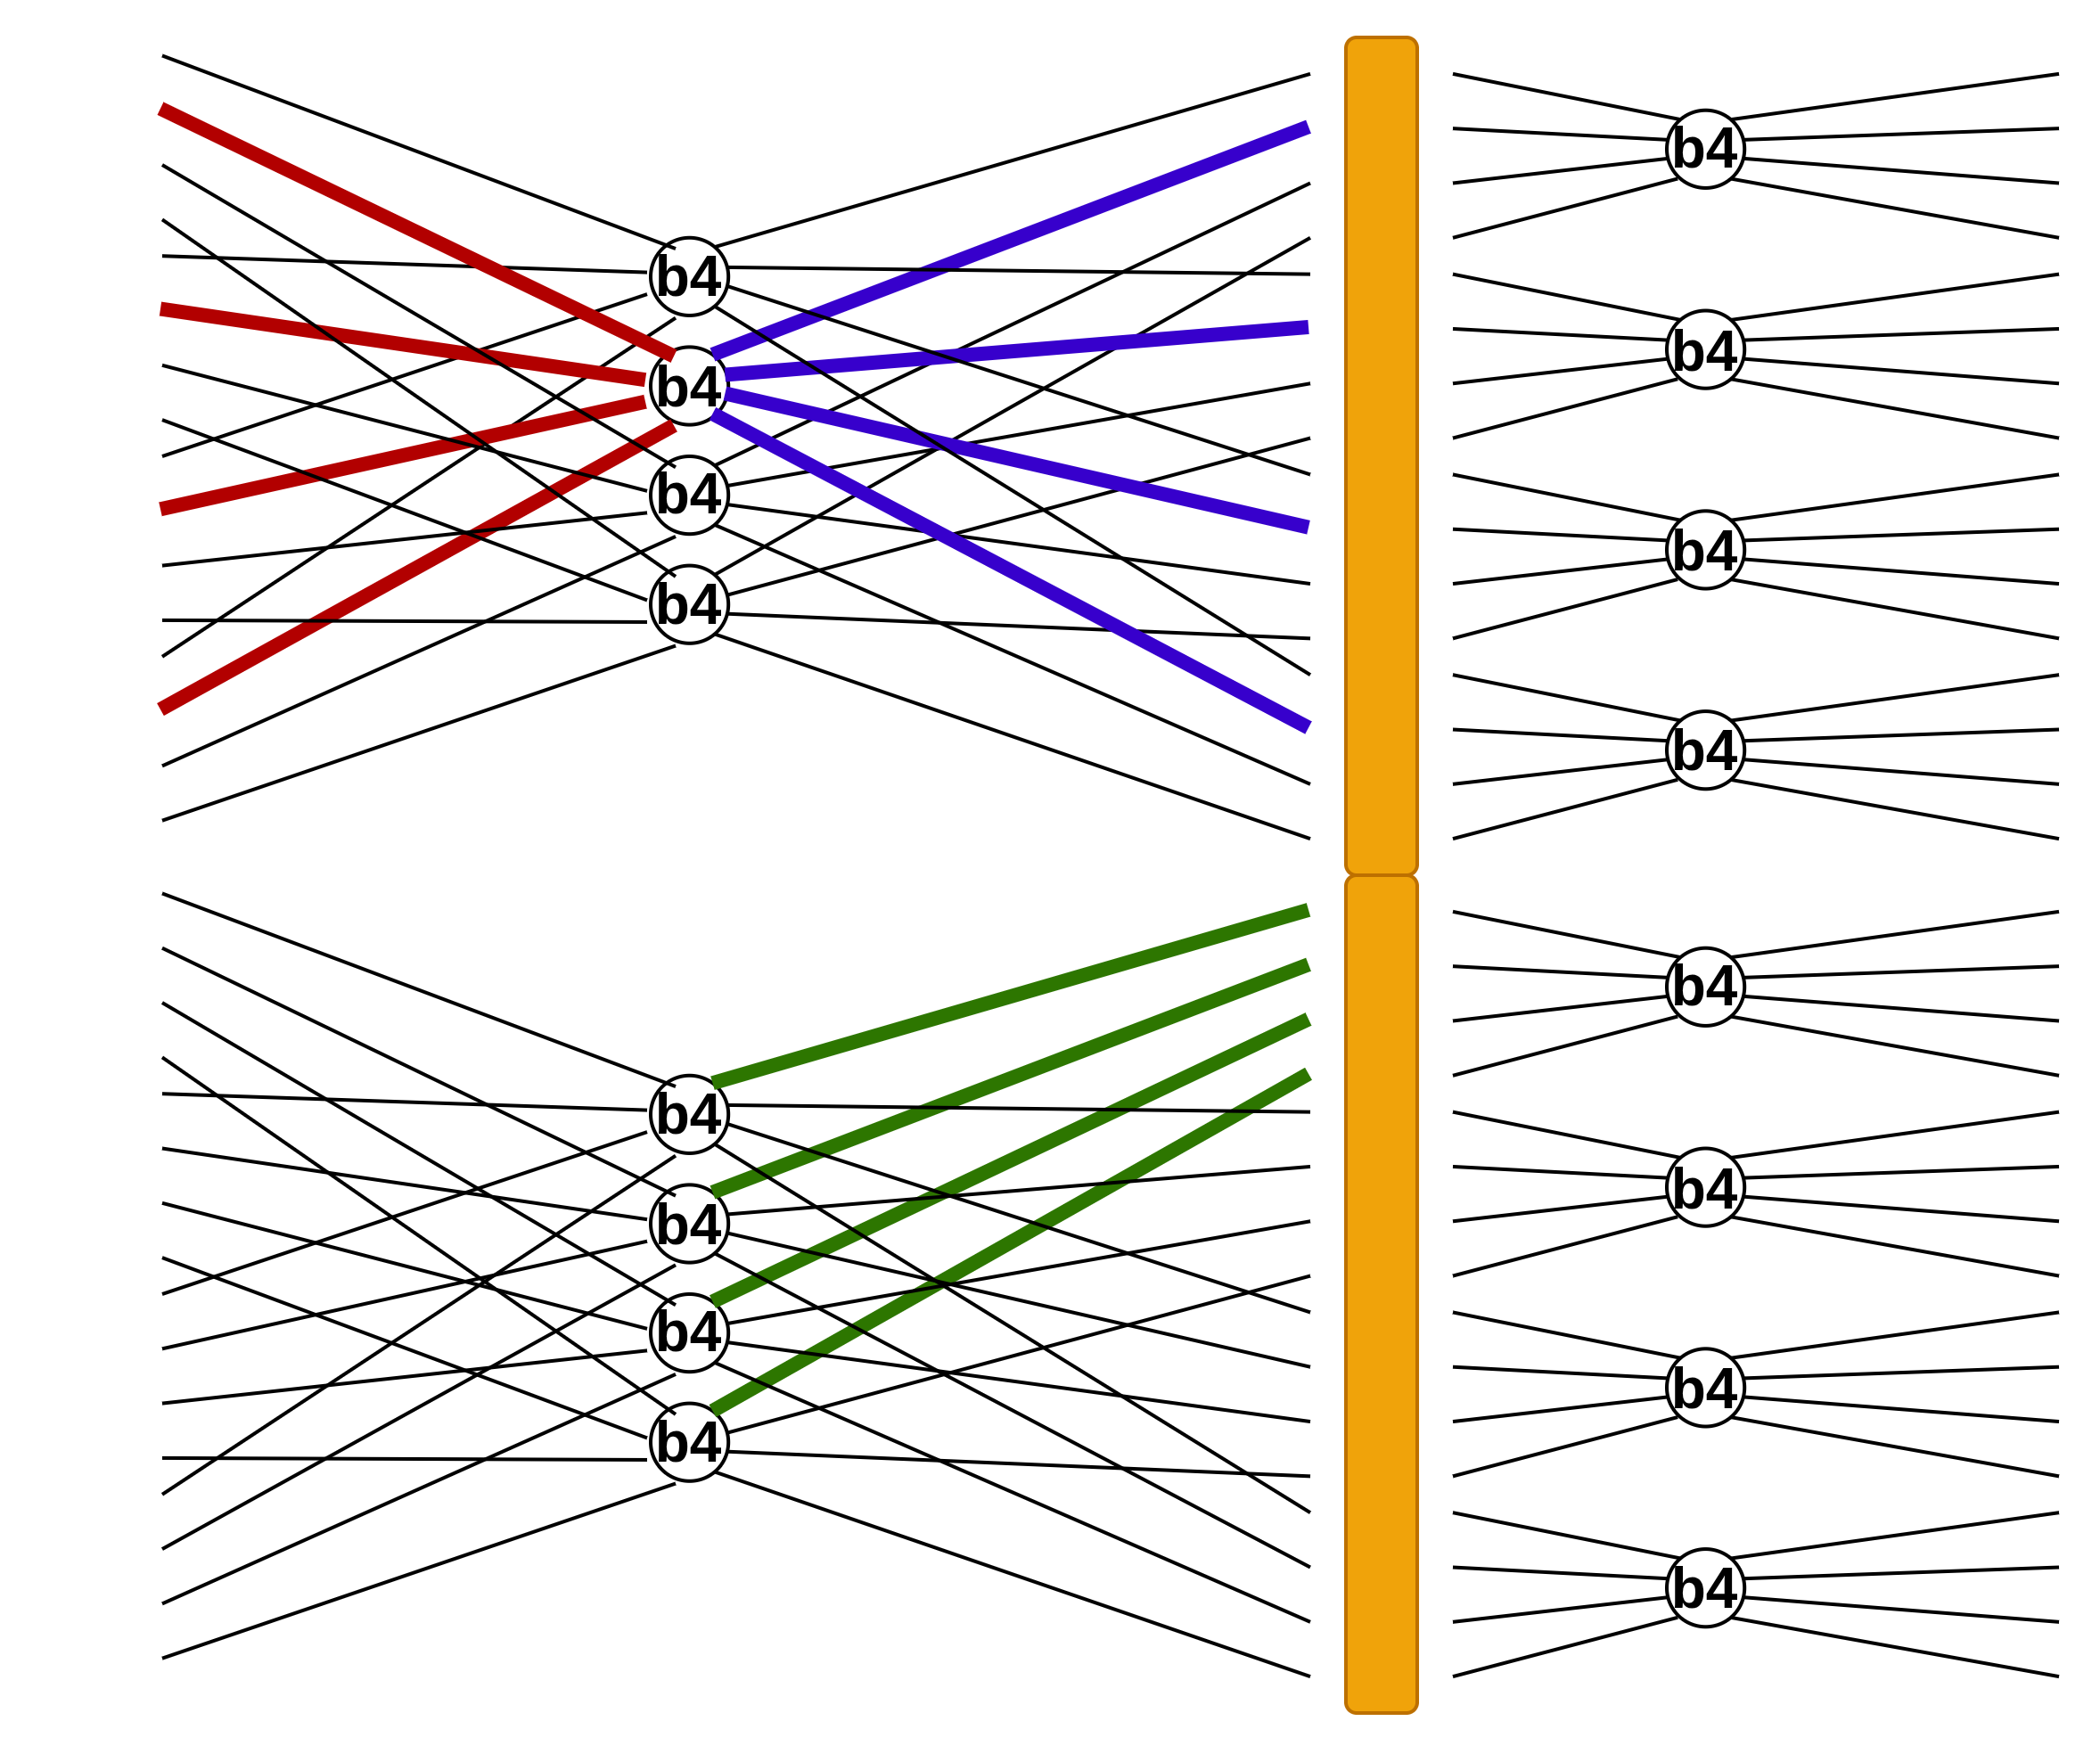
\includegraphics[width=\linewidth]{Images/5th_tetrada.png}
        \caption{Stride counter equals 00, butterfly counter 01}
        \label{fig:tetrada5}
    \end{subfigure}
    \hfill
    \begin{subfigure}[b]{0.3\linewidth}
        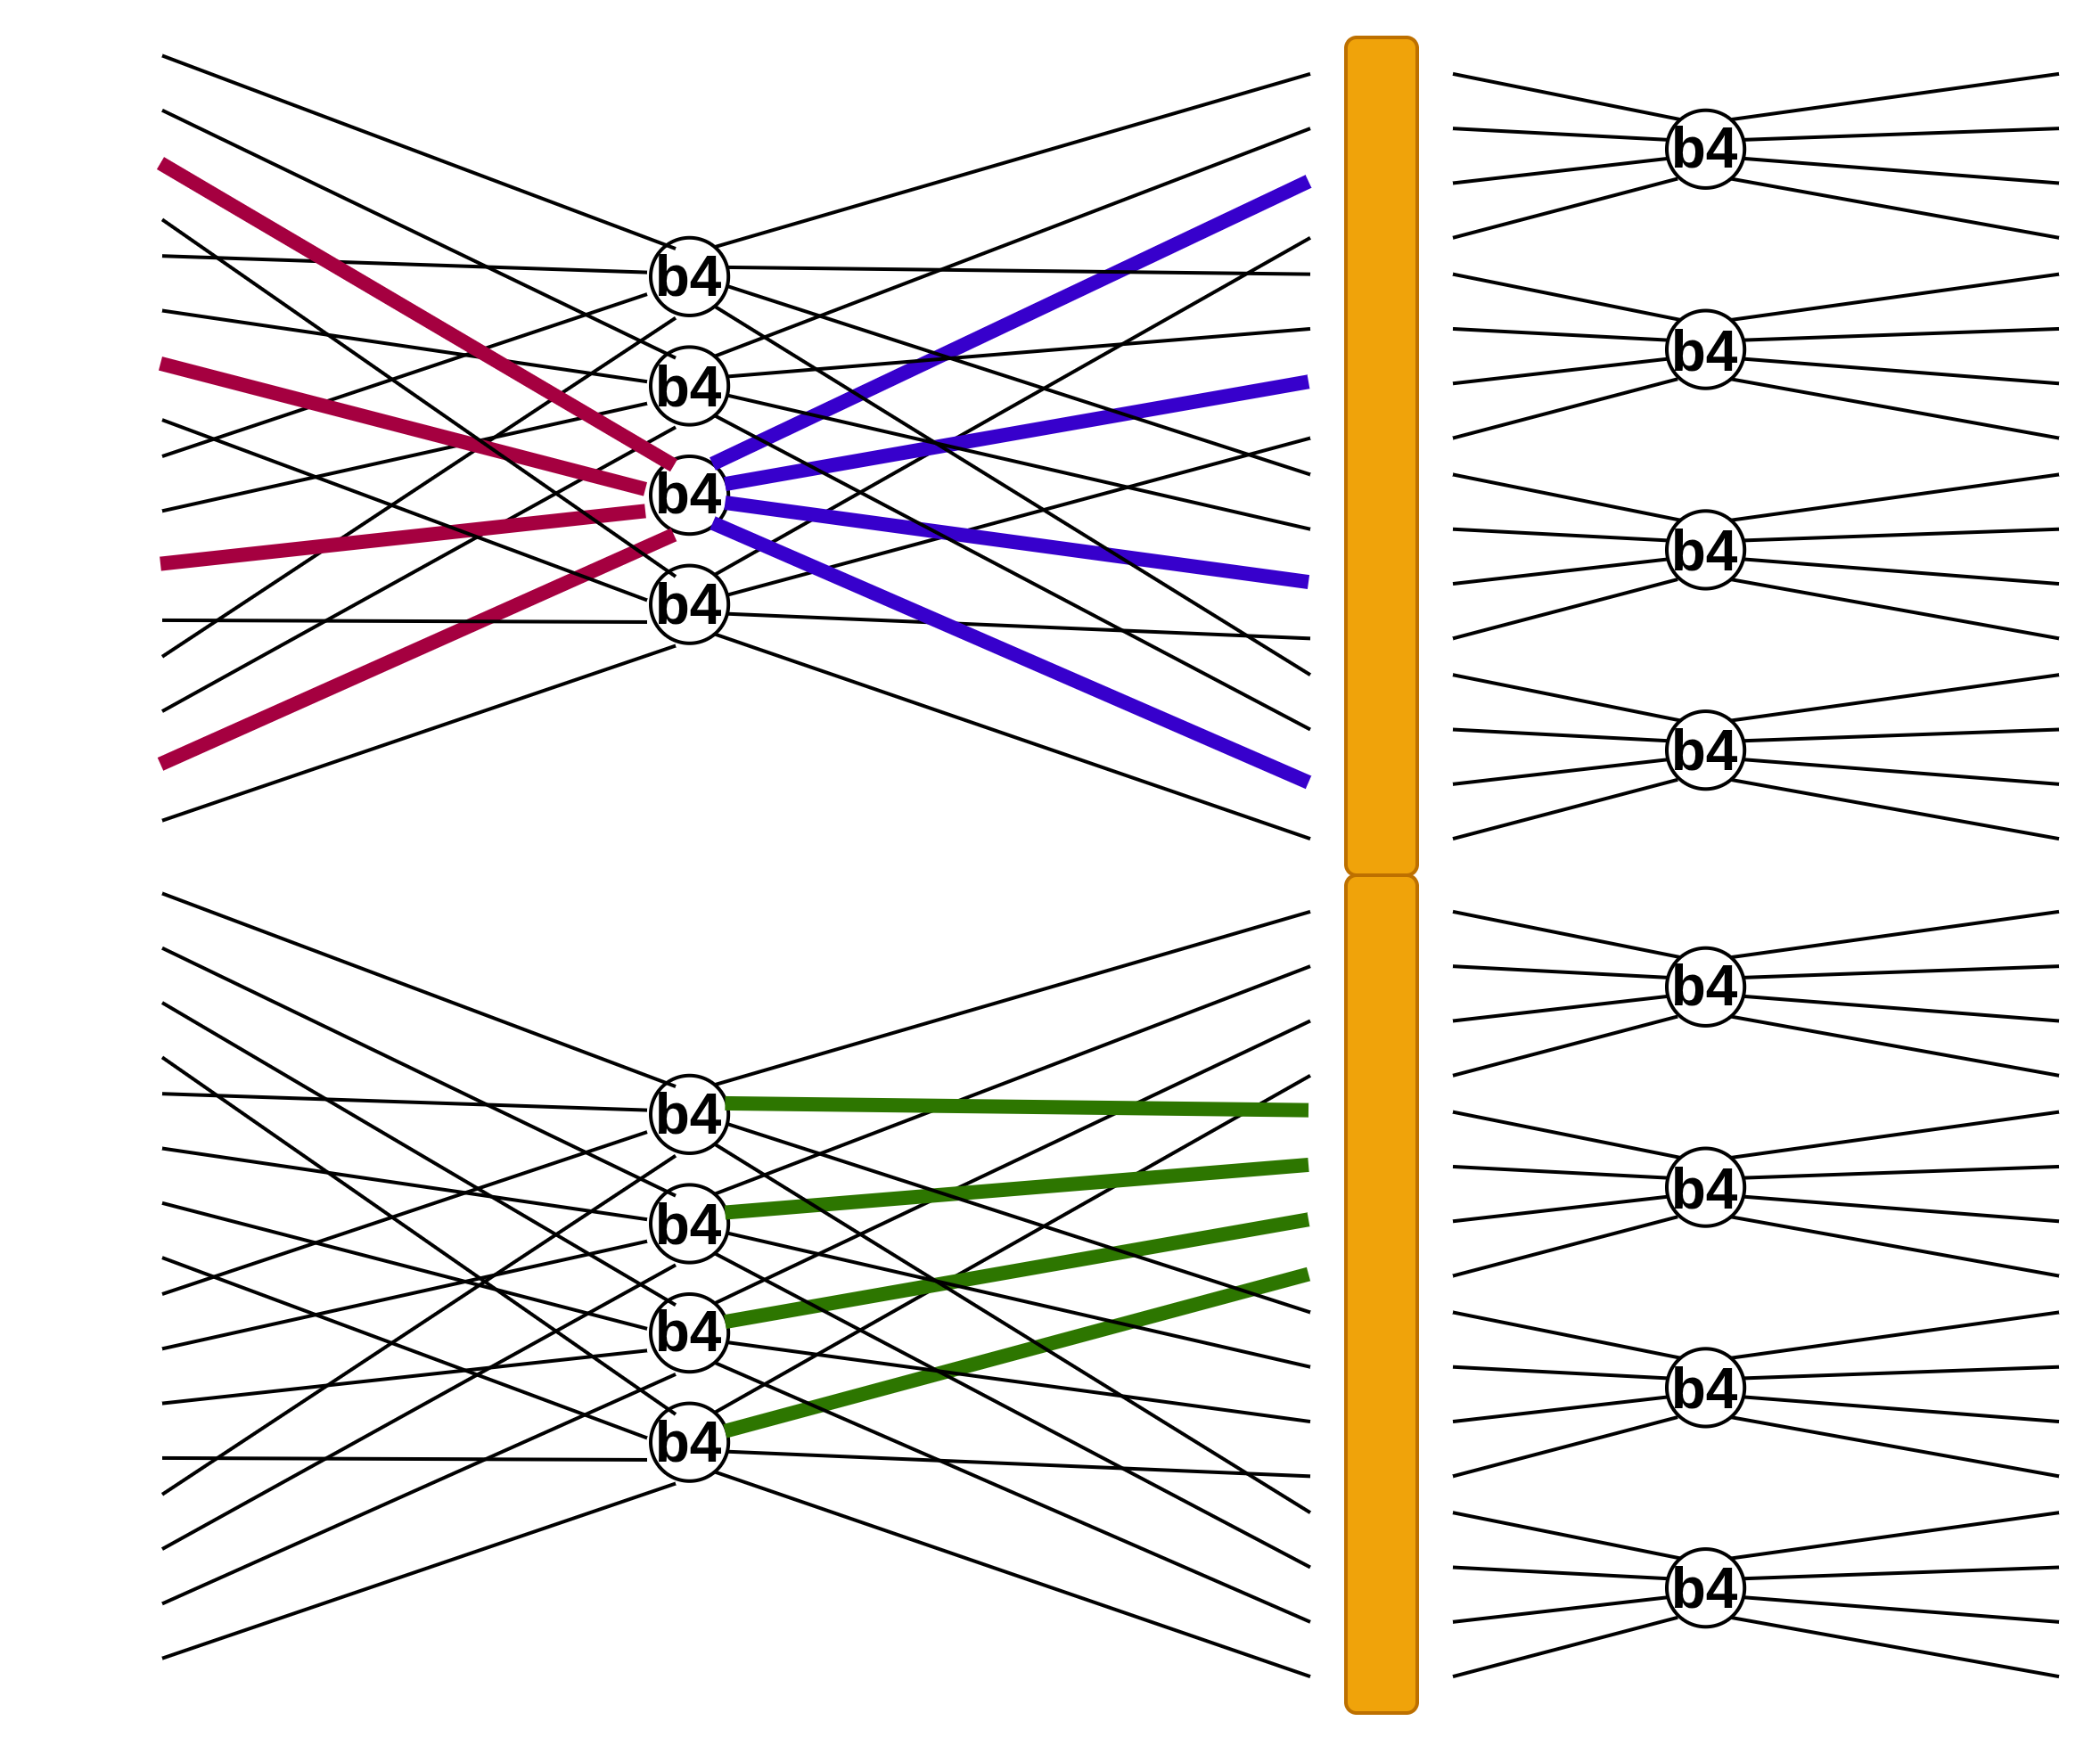
\includegraphics[width=\linewidth]{Images/6th_tetrada.png}
        \caption{Stride counter equals 01, butterfly counter 10}
        \label{fig:tetrada6}
    \end{subfigure}
    
    \caption{Operation flow of the counters managing the sets of four (quads) data points.}
    \label{fig:all_tetradas}
\end{figure}
\subsection{Delay Registers}

\subsection{}


    %\include{chapter...} % προσθέστε όσα χρειάζεται
    %\include{chapter_last}
%
%%%%%%%%%%%%%%%%%%%%%%%%%%%%%%%%%%%%%%%%%%%%%%%%%%%%


%\backmatter % μην ενεργοποιείτε την εντολή
% Βιβλιογραφία - Αναφορές
    \bibliographystyle{ieeetr}
	\bibliography{references}
    \nocite{*}


%%%%%%%%%%%%%%%%%%%%%%%%%%%%%%%%%%%%%%%%%%%%%%%%%%%%%
%% APPENDICES (optional) / ΠΑΡΑΡΤΗΜΑΤΑ (ΠΡΟΑΙΡΕΤΙΚΑ)
%%

% Εάν υπάρχουν περισσότερα από ένα Παραρτήματα
% είναι ενεργή η ακόλουθη εντολή
% και ανενεργή για μεμονωμένο Παράρτημα
    %% Να μην τροποποποιηθεί

\cleardoublepage\thispagestyle{plain}
~\vfill
\ifgrthesisoption
    \centerline{\huge\bf ΠΑΡΑΡΤΗΜΑΤΑ}\phantomsection
    \addcontentsline{toc}{chapter}{ΠΑΡΑΡΤΗΜΑΤΑ}
\else
    \centerline{\huge\bf APPENDICES}\phantomsection
    \addcontentsline{toc}{chapter}{APPENDICES}
\fi
\vfill

% Μην τροποποιήσετε τις ακόλουθες εντολές
\ifgrthesisoption
    \renewcommand{\chaptername}{Παράρτημα}
\else
    \renewcommand{\chaptername}{Appendix}
\fi

% Πριν το κάθε Παράρτημα (για περισσότερα από ένα), 
% ρυθμίζεται η κατάλληλη αλφαβητική αρίθμηση
%     \renewcommand{\thechapter}{A} 
%   	% Παράρτημα A

\chapter{Τίτλος Παραρτήματος \label{appendixA}}



Τα παραρτήματα περιλαμβάνουν συνοδευτικό, υποστηρικτικό υλικό (πίνακες, φωτογραφίες, ερωτηματολόγια, στατιστικά στοιχεία, αποδείξεις, περιγραφές  λογισμικών  προγραμμάτων,  παραδείγματα,  περιγραφές 
πολύπλοκων διαδικασιών, λίστα με πρωτογενή στοιχεία, λεπτομερής περιγραφή και προδιαγραφές εξοπλισμού, οδηγίες εγκατάστασης λογισμικού, κ.λπ.), ή αλλιώς ό,τι θεωρείται χρήσιμο να περιγραφεί, αλλά δεν συνηθίζεται να 
εντάσσεται μέσα στο κυρίως κείμενο της Εργασίας.  Στο κυρίως κείμενο της Εργασίας πρέπει να γίνονται οι κατάλληλες παραπομπές προς τα παραρτήματα, όπου το κείμενο σχετίζεται με υλικό που περιλαμβάνεται σε αυτά. Ένα παράρτημα, αναλόγως με το περιεχόμενό του, μπορεί να είναι ενιαίο, ή να χωρίζεται σε ενότητες.


\section{Δυνατότητες του \LaTeX}

Kαθώς το παρόν αποτελεί ένα πρότυπο συγγραφής διπλωματικών εργασιών, στην ενότητα αυτή επιδεικνύονται ορισμένες από τις δυνατότητες το \LaTeX οι οποίες μπορούν να αξιοποιηθούν στο κείμενο μιας διπλωματικής εργασίας (μια καλή πηγή για τη διερεύνηση των δυνατοτήτων του \LaTeX είναι η ιστοσελίδα {\small\url{https://www.overleaf.com/learn/latex/Main_Page}}).

\subsection{Πίνακες}
Ο Πίνακας~\ref{tab1} είναι ένα παράδειγμα πίνακα σχεδιασμένου με εντολές του περιβάλλοντος \texttt{tabular}.
\begin{table}[htb]
\centering
\caption{Παράμετροι πειραμάτων}
\label{tab1}
\begin{tabular}{|c|>{\centering\arraybackslash}m{8cm}|}
\hline Πλήθος κελιών καννάβου \textit{{c}} $\times$ \textit{{c}} & 50 $\times$ 50, 100 $\times$ 100, 200 $\times$ 200, \textbf{250} $\times$ \textbf{250}, 500 $\times$ 500, 1000 $\times$ 1000  \\
\hline Τυπική απόκλιση $\sigma$ & 25{m}, 50{m}, 75{m}, \textbf{100{m}}, 150{m}, 200{m} \\
\hline Αριθμός εγγύτερων γειτόνων \textit{{k}} & 1, 2, \textbf{3}, 4, 5, 10, 20 \\
\hline Πιθανοτικό κατώφλι $\theta$ & 50$\%$, 60$\%$, 70$\%$, \textbf{75$\%$}, 80$\%$, 90$\%$, 99$\%$ \\
\hline  
\end{tabular}

\end{table} 

\subsection{Διαγράμματα - Γραφικές παραστάσεις}
Στο Σχήμα~\ref{fig1}, παρουσιάζεται ένα παράδειγμα γραφικής παράστασης σχεδιασμένης με το Gnuplot. Ένας άλλος τρόπος κατασκευής τέτοιων παραστάσεων/διαγραμμάτων είναι με χρήση του πακέτου pgfplots (\url{http://pgfplots.sourceforge.net/}).
\begin{figure}[htb]
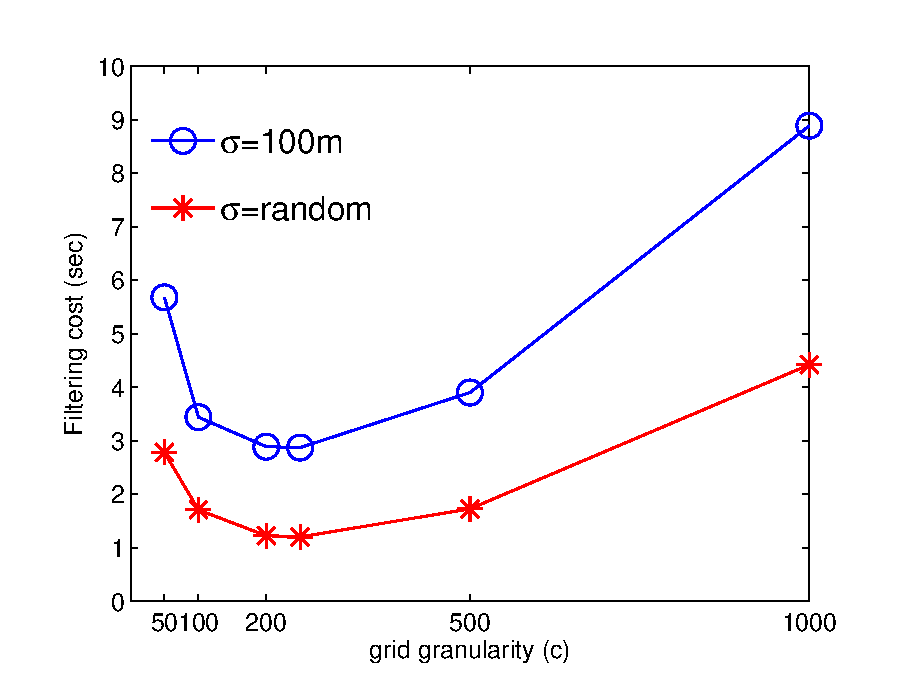
\includegraphics[scale=0.7]{figures/grid_granularity.eps}
\centering
\caption{Κλιμάκωση χρόνου εκτέλεσης για διάφορες υποδιαιρέσεις του καννάβου}	
\label{fig1}
\end{figure} 

Στο Σχήμα~\ref{Quadtree}, παρουσιάζεται ένα παράδειγμα εισαγωγής σχήματος/εικόνας που περιέχεται σε αρχείο pdf, ενώ στο Κεφάλαιο \ref{chap2}, στο Σχήμα \ref{dataconnection} παρουσιάζεται ένα παράδειγμα εισαγωγής σχήματος/εικόνας που περιέχεται σε αρχείο jpg.
\begin{figure}[htb]
\centering
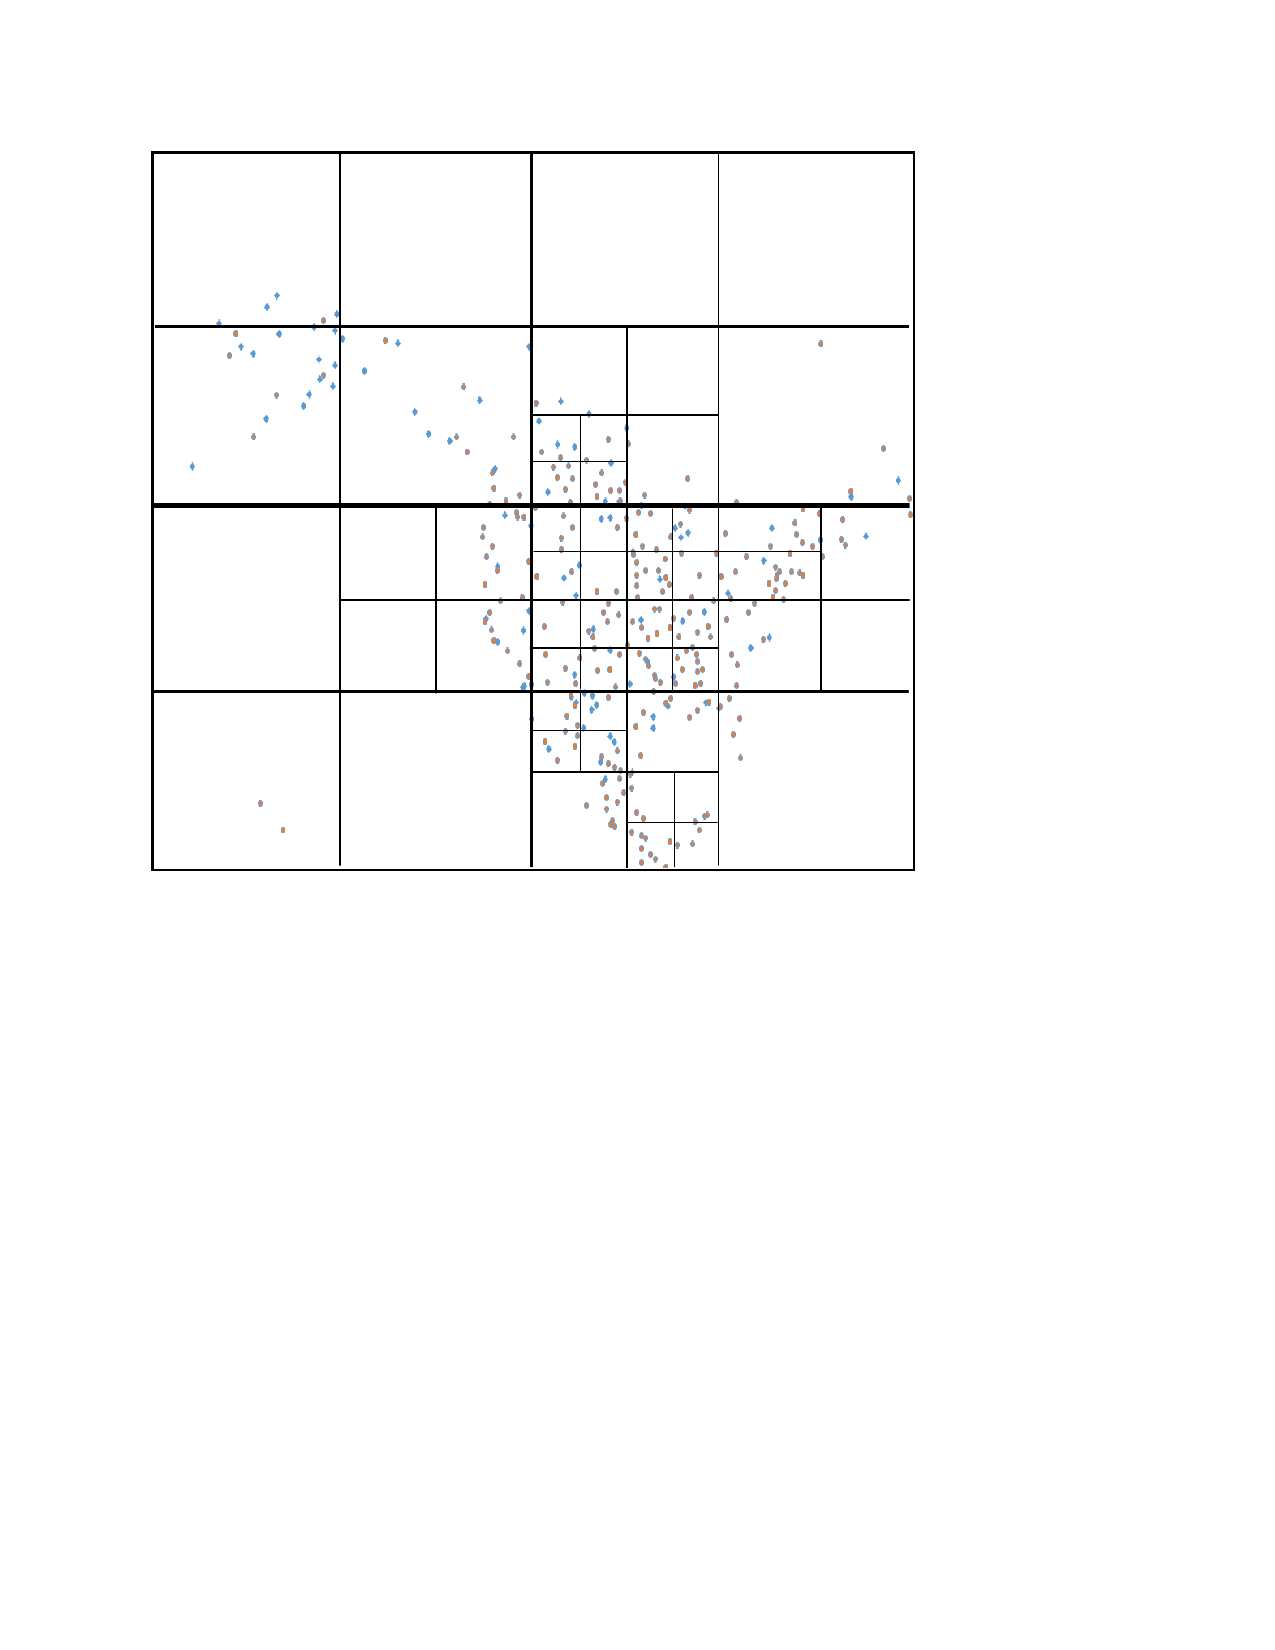
\includegraphics[width = 0.57\columnwidth, height = 8.5cm ]{figures/quadtree.pdf}
\caption{Quadtree partitioning.}
\label{Quadtree}
\end{figure}

\subsection{Σχήματα}
Ακολουθεί στο Σχήμα~\ref{fig2} ένα παράδειγμα σχήματος φτιαγμένου με εντολές του πακέτου Ti\textit{k}Z.
\begin{figure}[htb]
\begin{center}
\begin{tikzpicture}
\draw (-2,0) -- (2,0);
\filldraw [gray] (0,0) circle (2pt);
\draw (-2,-2) .. controls (0,0) .. (2,-2);
%\draw (-2,2) .. controls (-1,0) and (1,0) .. (2,2);
 \draw[gray, thick] (-1,2) -- (2,-4);
\draw[gray, thick] (-1,-1) -- (2,2);
\filldraw[black] (0,0) circle (2pt)  ;
\end{tikzpicture}
\end{center}
\caption{Παράδειγμα σχήματος με εντολές του πακέτου Ti\textit{k}Z}	
\label{fig2}
\end{figure}

\subsection{Μαθηματικές εκφράσεις}
Ακολουθούν παραδείγματα μαθηματικών εκφράσεων.
\begin{eqnarray}
\hat{I}(x,u,t)     &=& dist(y(t_f),\Gamma)
+  \int_t^{t_f} \: {\cal L}( y(s),u(s),s) \: ds
\label{con11b}
\end{eqnarray}

     \[
        \frac{d}{dx}\left( \int_{0}^{z} f(u)\,du\right)=f(x).
     \]

\subsection{Αλγόριθμοι}
Ακολουθεί ο Αλγόριθμος~\ref{alg1}, ο οποίος είναι μορφοποιημένος με τα πακέτα algorithm και algorithmic.

\begin{algorithm}[htb]
\caption{\ \ \ Probabilistic $k\theta NN$ Monitoring}
\begin{algorithmic}[1]
\begin{small}

\STATE{\bf Procedure} {\em VerifyCandidate} (focal query point $q$, threshold $\theta$, object $o$, list of auxiliary objects $P$, distance $kMAXDIST$) 

\IF { $\Phi(o, kMAXDIST) \geq \theta$ {\bf and} $L_2(q, o) \leq L_2(q, P.$top()) }

\STATE {$P$.pop()};   \ \ \ \ \ \ \ \ {\em //Replace the most extreme element in $P$, since candidate $o$ ... }

\STATE {$P$.push($o$)};  \ \ \ \ \ {\em //... has enough probability and has its mean closer to focal $q$ }

\ENDIF

\STATE {\bf End Procedure}


\end{small}
\end{algorithmic}
\label{alg1}
\end{algorithm}

\subsection{Θεωρήματα, Πορίσματα, Ορισμοί, κλπ.}

Ακολουθεί παράδειγμα θεωρήματος από την ιστοσελίδα  {\small\url{https://www.overleaf.com/learn/latex/Theorems_and_proofs}}

\begin{theorem}
Let $f$ be a function whose derivative exists in every point, then $f$ 
is a continuous function.
\end{theorem}

\subsection{Απαριθμήσεις}

Μια απαρίθμηση (itemized list) βοηθά στην παρουσίαση μιας σειράς περιπτώσεων με σαφήνεια.
Ακολουθεί παράδειγμα.

H εκπαίδευση στην Ελλάδα διακρίνεται σε:
\begin{itemize}
\item Πρωτοβάθμια 
\item Δευτεροβάθμια 
\item Τριτοβάθμια 
\end{itemize}

\subsection{Είδη πηγών στις αναφορές}

Στο references.bib μπορεί να δει κανείς πώς γράφονται διάφορα είδη πηγών 
(Βιβλία Ξενόγλωσσα \cite{goossens93},
Βιβλία Ελληνικά \cite{greekbook},
Άρθρα σε επιστημονικά περιοδικά \cite{LiArTs13},
Άρθρα σε επιστημονικά συνέδρια \cite{dcis2011},
Ιστοσελίδες \cite{LaTeXProject},
Πτυχιακές Εργασίες \cite{elli05},
Διπλωματικές Εργασίες \cite{zoi04},
Μεταπτυχιακές Διπλωματικές Εργασίες \cite{master04},
Διδακτορικές Διατριβές \cite{phd045},
Τεχνικές Αναφορές \cite{MSU-CSE-05-29},
Διπλώματα Ευρεσιτεχνίας \cite{viswanathan2014convenient}),
Κεφάλαια σε συλλογικούς τόμους
\cite{[PS11]}.

	
% % %	
%     \renewcommand{\thechapter}{B}
%     % Παράρτημα B

 
\chapter{Τίτλος 2ου Παραρτήματος\label{appendixB}}

Τα παραρτήματα περιλαμβάνουν συνοδευτικό, υποστηρικτικό υλικό (πίνακες, φωτογραφίες, ερωτηματολόγια, στατιστικά στοιχεία, αποδείξεις, περιγραφές  λογισμικών  προγραμμάτων,  παραδείγματα,  περιγραφές 
πολύπλοκων διαδικασιών, λίστα με πρωτογενή στοιχεία, λεπτομερής περιγραφή και προδιαγραφές εξοπλισμού, οδηγίες εγκατάστασης λογισμικού, κ.λπ.), ή αλλιώς ό,τι θεωρείται χρήσιμο να περιγραφεί, αλλά δεν συνηθίζεται να 
εντάσσεται μέσα στο κυρίως κείμενο της Εργασίας.  Στο κυρίως κείμενο της Εργασίας πρέπει να γίνονται οι κατάλληλες παραπομπές προς τα παραρτήματα, όπου το κείμενο σχετίζεται με υλικό που περιλαμβάνεται σε αυτά. Ένα παράρτημα, αναλόγως με το περιεχόμενό του, μπορεί να είναι ενιαίο, ή να χωρίζεται σε ενότητες.

% Εάν υπάρχει μόνο ένα Παράρτημα,
% μπαίνουν σε σχόλια οι παραπάνω γραμμές 
% και ρυθμίζεται αρίθμηση χωρίς γράμμα
%   \renewcommand{\thechapter}{} 
%   \renewcommand{\thesection}{\arabic{section}}
%
% Ακολουθεί αρχείο μεμονωμένου Παραρτήματος
% (διαφορετική δομή από appA/appΒ)
%   % Μεμονωμένο Παράρτημα 
% ορίζεται ο τίτλος του παραρτήματος
\edef\chaptertitle{Τίτλος Παραρτήματος}
\label{appendix}

% Μην τροποποιήσετε τις ακόλουθες εντολές
\chapter*{\chaptername\\\vspace{1cm} \chaptertitle} 
\addcontentsline{toc}{chapter}{\chaptername\texorpdfstring{\\}~\chaptertitle}
\setcounter{section}{0}
\renewcommand{\chaptermark}[1]{\markboth{\textit{\chaptername. \chaptertitle}}{}}
\chaptermark{}


Τα παραρτήματα περιλαμβάνουν συνοδευτικό, υποστηρικτικό υλικό (πίνακες, φωτογραφίες, ερωτηματολόγια, στατιστικά στοιχεία, αποδείξεις, περιγραφές  λογισμικών  προγραμμάτων,  παραδείγματα,  περιγραφές 
πολύπλοκων διαδικασιών, λίστα με πρωτογενή στοιχεία, λεπτομερής περιγραφή και προδιαγραφές εξοπλισμού, οδηγίες εγκατάστασης λογισμικού, κ.λπ.), ή αλλιώς ό,τι θεωρείται χρήσιμο να περιγραφεί, αλλά δεν συνηθίζεται να 
εντάσσεται μέσα στο κυρίως κείμενο της Εργασίας.  Στο κυρίως κείμενο της Εργασίας πρέπει να γίνονται οι κατάλληλες παραπομπές προς τα παραρτήματα, όπου το κείμενο σχετίζεται με υλικό που περιλαμβάνεται σε αυτά. Ένα παράρτημα, αναλόγως με το περιεχόμενό του, μπορεί να είναι ενιαίο, ή να χωρίζεται σε ενότητες.


\section{Δυνατότητες του \LaTeX}

Kαθώς το παρόν αποτελεί ένα πρότυπο συγγραφής διπλωματικών εργασιών, στην ενότητα αυτή επιδεικνύονται ορισμένες από τις δυνατότητες το \LaTeX οι οποίες μπορούν να αξιοποιηθούν στο κείμενο μιας διπλωματικής εργασίας (μια καλή πηγή για τη διερεύνηση των δυνατοτήτων του \LaTeX είναι η ιστοσελίδα {\small\url{https://www.overleaf.com/learn/latex/Main_Page}}).

\subsection{Πίνακες}
Ο Πίνακας~\ref{tab1} είναι ένα παράδειγμα πίνακα σχεδιασμένου με εντολές του περιβάλλοντος \texttt{tabular}.
\begin{table}[htb]
\centering
\caption{Παράμετροι πειραμάτων}
\label{tab1}
\begin{tabular}{|c|>{\centering\arraybackslash}m{8cm}|}
\hline Πλήθος κελιών καννάβου \textit{{c}} $\times$ \textit{{c}} & 50 $\times$ 50, 100 $\times$ 100, 200 $\times$ 200, \textbf{250} $\times$ \textbf{250}, 500 $\times$ 500, 1000 $\times$ 1000  \\
\hline Τυπική απόκλιση $\sigma$ & 25{m}, 50{m}, 75{m}, \textbf{100{m}}, 150{m}, 200{m} \\
\hline Αριθμός εγγύτερων γειτόνων \textit{{k}} & 1, 2, \textbf{3}, 4, 5, 10, 20 \\
\hline Πιθανοτικό κατώφλι $\theta$ & 50$\%$, 60$\%$, 70$\%$, \textbf{75$\%$}, 80$\%$, 90$\%$, 99$\%$ \\
\hline  
\end{tabular}

\end{table}

\subsection{Διαγράμματα - Γραφικές παραστάσεις}
Στο Σχήμα~\ref{fig1}, παρουσιάζεται ένα παράδειγμα γραφικής παράστασης σχεδιασμένης με το Gnuplot.
\begin{figure}[htb]
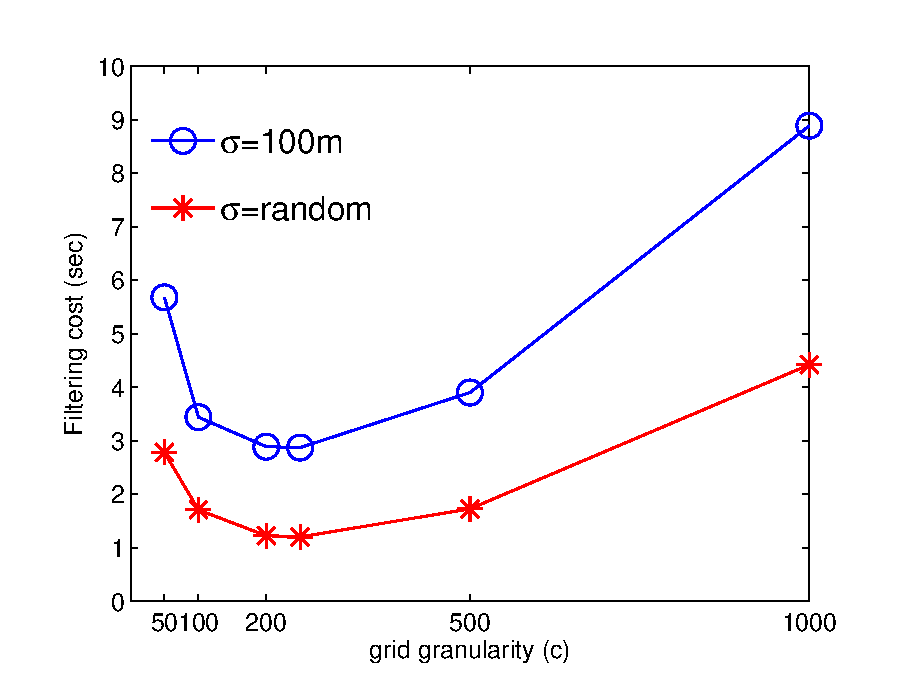
\includegraphics[scale=0.7]{figures/grid_granularity.eps}
\centering
\caption{Κλιμάκωση χρόνου εκτέλεσης για διάφορες υποδιαιρέσεις του καννάβου}	
\label{fig1}
\end{figure} 

\subsection{Σχήματα}
Ακολουθεί στο Σχήμα~\ref{fig2} ένα παράδειγμα σχήματος φτιαγμένου με εντολές του πακέτου Ti\textit{k}Z.
\begin{figure}[htb]
\begin{center}
\begin{tikzpicture}
\draw (-2,0) -- (2,0);
\filldraw [gray] (0,0) circle (2pt);
\draw (-2,-2) .. controls (0,0) .. (2,-2);
%\draw (-2,2) .. controls (-1,0) and (1,0) .. (2,2);
 \draw[gray, thick] (-1,2) -- (2,-4);
\draw[gray, thick] (-1,-1) -- (2,2);
\filldraw[black] (0,0) circle (2pt)  ;
\end{tikzpicture}
\end{center}
\caption{Παράδειγμα σχήματος με εντολές του πακέτου Ti\textit{k}Z}	
\label{fig2}
\end{figure}

\subsection{Αλγόριθμοι}
Ακολουθεί ο Αλγόριθμος~\ref{alg1}, ο οποίος είναι μορφοποιημένος με τα πακέτα algorithm και algorithmic.

\begin{algorithm}[htb]
\caption{\ \ \ Probabilistic $k\theta NN$ Monitoring}
\begin{algorithmic}[1]
\begin{small}

\STATE{\bf Procedure} {\em VerifyCandidate} (focal query point $q$, threshold $\theta$, object $o$, list of auxiliary objects $P$, distance $kMAXDIST$) 

\IF { $\Phi(o, kMAXDIST) \geq \theta$ {\bf and} $L_2(q, o) \leq L_2(q, P.$top()) }

\STATE {$P$.pop()};   \ \ \ \ \ \ \ \ {\em //Replace the most extreme element in $P$, since candidate $o$ ... }

\STATE {$P$.push($o$)};  \ \ \ \ \ {\em //... has enough probability and has its mean closer to focal $q$ }

\ENDIF

\STATE {\bf End Procedure}


\end{small}
\end{algorithmic}
\label{alg1}
\end{algorithm}

\subsection{Μαθηματικές εκφράσεις}
Ακολουθούν παραδείγματα μαθηματικών εκφράσεων.
\begin{eqnarray}
\hat{I}(x,u,t)     &=& dist(y(t_f),\Gamma)
+  \int_t^{t_f} \: {\cal L}( y(s),u(s),s) \: ds
\label{con11b}
\end{eqnarray}

     \[
        \frac{d}{dx}\left( \int_{0}^{z} f(u)\,du\right)=f(x).
     \]

\subsection{Θεωρήματα, Πορίσματα, Ορισμοί, κλπ.}

Ακολουθεί παράδειγμα θεωρήματος από την ιστοσελίδα  {\small\url{https://www.overleaf.com/learn/latex/Theorems_and_proofs}}

\begin{theorem}
Let $f$ be a function whose derivative exists in every point, then $f$ 
is a continuous function.
\end{theorem}

\subsection{Απαριθμήσεις}

Μια απαρίθμηση (itemized list) βοηθά στην παρουσίαση μιας σειράς περιπτώσεων με σαφήνεια.
Ακολουθεί παράδειγμα.

H εκπαίδευση στην Ελλάδα διακρίνεται σε:
\begin{itemize}
\item Πρωτοβάθμια 
\item Δευτεροβάθμια 
\item Τριτοβάθμια 
\end{itemize}

\subsection{Είδη πηγών στις αναφορές}

Στο references.bib μπορεί να δει κανείς πώς γράφονται διάφορα είδη πηγών 
(Βιβλία Ξενόγλωσσα \cite{goossens93},
Βιβλία Ελληνικά \cite{greekbook},
Άρθρα σε επιστημονικά περιοδικά \cite{LiArTs13},
Άρθρα σε επιστημονικά συνέδρια \cite{dcis2011},
Ιστοσελίδες \cite{LaTeXProject},
Πτυχιακές Εργασίες \cite{elli05},
Διπλωματικές Εργασίες \cite{zoi04},
Μεταπτυχιακές Διπλωματικές Εργασίες \cite{master04},
Διδακτορικές Διατριβές \cite{phd045},
Τεχνικές Αναφορές \cite{MSU-CSE-05-29},
Διπλώματα Ευρεσιτεχνίας \cite{viswanathan2014convenient}),
Κεφάλαια σε συλλογικούς τόμους
\cite{[PS11]}.

 

%
%%%%%%%%%%%%%%%%%%%%%%%%%%%%%%%%%%%%%%%%%%%%%%%%%%%%


\end{document}